% report/ExpBmain000.tex
\documentclass[18pt,c]{beamer}
\makeatletter
\let\beamer@writeslidentry@miniframeson=\beamer@writeslidentry
\def\beamer@writeslidentry@miniframesoff{%
  \expandafter\beamer@ifempty\expandafter{\beamer@framestartpage}{}% does not happen normally
  {%else
    % removed \addtocontents commands
   \clearpage\beamer@notesactions%
  }
}
\newcommand*{\miniframeson}{\let\beamer@writeslidentry=\beamer@writeslidentry@miniframeson}
\newcommand*{\miniframesoff}{\let\beamer@writeslidentry=\beamer@writeslidentry@miniframesoff}
\makeatother
% yellow
\definecolor{goldenyellow}{rgb}{1.0, 0.87, 0.0}
\definecolor{electricyellow}{rgb}{1.0, 1.0, 0.0}
\definecolor{icterine}{rgb}{0.99, 0.97, 0.37}
\definecolor{flavescent}{rgb}{0.97, 0.91, 0.56}
\definecolor{lemon}{rgb}{1.0, 0.97, 0.0}
% orange
\definecolor{amber}{rgb}{1.0, 0.75, 0.0}
\definecolor{cadmiumorange}{rgb}{0.93, 0.53, 0.18}
\definecolor{internationalorange}{rgb}{1.0, 0.31, 0.0}
% red
\definecolor{ferrarired}{rgb}{1.0, 0.11, 0.0}
\definecolor{fireenginered}{rgb}{0.81, 0.09, 0.13}
\definecolor{cadmiumred}{rgb}{0.89, 0.0, 0.13}
% blue
\definecolor{ao}{rgb}{0.0, 0.5, 0.0}
\definecolor{babyblueeyes}{rgb}{0.63, 0.79, 0.95}
\definecolor{bleudefrance}{rgb}{0.19, 0.55, 0.91}
\definecolor{blue}{rgb}{0.0, 0.0, 1.0}
\definecolor{cobalt}{rgb}{0.0, 0.28, 0.67}
\definecolor{darkmidnightblue}{rgb}{0.0, 0.2, 0.4}
\definecolor{brandeisblue}{rgb}{0.0, 0.44, 1.0}
\definecolor{deepskyblue}{rgb}{0.0, 0.75, 1.0}
\definecolor{iris}{rgb}{0.35, 0.31, 0.81}
\definecolor{navyblue}{rgb}{0.0, 0.0, 0.5}
\definecolor{ultramarine}{rgb}{0.07, 0.04, 0.56}
\definecolor{electricultramarine}{rgb}{0.25, 0.0, 1.0}
% green
\definecolor{cadmiumgreen}{rgb}{0.0, 0.42, 0.24}
\definecolor{darkpastelgreen}{rgb}{0.01, 0.75, 0.24}
\usetheme{Antibes}
\usecolortheme{default}
\usefonttheme{default}
\setbeamercolor{structure}{fg=deepskyblue}
\setbeamerfont{frametitle}{size=\footnotesize}
\usepackage{graphicx}
\renewcommand{\topfraction}{1.0}
\renewcommand{\floatpagefraction}{1.0}
\begin{document}
\title{Report of Experiment ExpB. k-Symmetry: Grammar Tuning}
\author{Andreas Geyer-Schulz}
\date{\today}
\begin{frame}
\titlepage
\end{frame}
\begin{frame}
\frametitle{Abstract}
Context-free grammars control the stochastic process for generating programs in grammar-based genetic programming algorithms. The stochastic process can be tuned by adding additional production rules. In this experiment we compare 4 manually tuned grammars for boolean functions with a standard grammar for boolean functions for learning k-symmetry problems. Grammar tuning (the grammar dimension) is a distinctive feature of grammar-based genetic programming.%\end{abstract}
\end{frame}
\begin{frame}[t, allowframebreaks]
\frametitle{Contents}
\tableofcontents[subsubsectionstyle=hide]
\vfill
\end{frame}
% report/ExpBmain001.tex
\begin{frame}
\vspace*{2mm}
\begin{block}{
Definition
}
{\bf Grammar tuning} means adding additional production rules
to a context-free grammar with the goal of improving the learning
performance of grammar-based genetic programming algorithms.
 
{\bf Example:} Repeating production rules allows to change the distribution
of programs (and their sizes) generated during the initialization of a grammar-based
genetic programming algorithm.
\end{block}
\end{frame}% report/ExpBmain002.tex
\begin{frame}
\vspace*{2mm}
\begin{block}{
Definition
}
{\bf Families of functions} are parametrized functions whose difficulty
can be controlled by one or more parameters.
 
{\bf Example:} The family of k-symmetry functions.
The k-symmetry problem requires finding a function which classifies
a k-bit string as symmetric.
The parameter $k$ defines the length of the bit string.
The problem is NP hard, because the number of test cases increases by $2^k$.
\end{block}
\end{frame}% report/ExpBmain003.tex
\begin{frame}
\vspace*{2mm}
\begin{block}{
Description of Experiment
}
The purpose of this computational experiment is to show the improvement
of performance by grammar tuning.
 
The {\bf problem environment} is the k-symmetry problem: 
Finding a boolean expression (with and, or, and not)
which is TRUE for symmetric k-bit strings.
 
The {\bf solution method} is grammar-based genetic programming
(option {\tt algorithm="sgp"}  of {\tt xegaRun}).
The {\bf solver} used is {\tt xegaRun} from the R-package {\tt xega}.
 
The experiment consists of 25 treatments, 5 grammars for 5 problem sizes $k\in 2,\dots, 6$.
\end{block}
\end{frame}% report/ExpBmain004.tex
\begin{frame}
\frametitle{
Description of Experiment
}
The two control variables in this experiment are
\begin{itemize}
\item The bit-length of the k-symmetry problem: 2, 3, 4, 5, and 6.
\item The grammar for boolean expressions:
\begin{itemize} 
\item {\bf T0}: A standard grammar for boolean expressions.
\item {\bf T1}: A standard grammar for boolean expressions.
            With two rules for OR and a rule for a template 
            which tests for the symmetry of two bits.
\item {\bf T2}: With two rules for AND and one rule for variables replaced
            by symmetric pairs.
\item {\bf T3}: With two rules for OR and one rule variables replaced
            by symmetric pairs.
\item {\bf T4}: With two rules for OR and two rules for variables replaced
            by symmetric pairs.
\end{itemize}
\end{itemize}
\end{frame}% report/ExpBmain005.tex
\miniframeson
\section{Design of Experiment}
% report/ExpBmain006.tex
% ExpB
% Table: Common Parameters of Experiment ExpB
% Fri May  9 19:04:39 2025
 \begin{frame}
 \fontsize{8pt}{9pt}\selectfont
 \frametitle{ Common Parameters of Experiment ExpB }
% latex table generated in R 4.4.3 by xtable 1.8-4 package
% Fri May  9 19:04:39 2025
\begin{table}[ht]
\centering
\begin{tabular}{rr}
  \hline
 & Parameter Value \\ 
  \hline
Experiment & EB \\ 
  Optimize & Minimize! \\ 
  Trials & 80 \\ 
  Algorithm & sgp \\ 
  Max.Depth.of.DTs & 7 \\ 
  Replay & 0 \\ 
  Evaluation.Method & Deterministic \\ 
  Execution.Model & MultiCore \\ 
  Verbose & 1 \\ 
  Semantics & byValue \\ 
  Report.Eval.Errors & TRUE \\ 
  Termination.Condition & AbsoluteError \\ 
  Termination.Eps & -0.1 \\ 
  Gene.Map & Bin2Dec \\ 
  Init.Gene & InitGene \\ 
   \hline
\end{tabular}
\caption{Common Parameters of Experiment ExpB (Part 1)} 
\end{table}

 \label{ExpBCommonTable000.tex}  
 \end{frame}

 % Label:  \label{ExpBCommonTable000.tex}  
% report/ExpBmain007.tex
% ExpB
% Table: Common Parameters of Experiment ExpB
% Fri May  9 19:04:39 2025
 \begin{frame}
 \fontsize{8pt}{9pt}\selectfont
 \frametitle{ Common Parameters of Experiment ExpB }
\input{ExpBCommonTable001.tex}
 \label{ExpBCommonTable001.tex}  
 \end{frame}

 % Label:  \label{ExpBCommonTable001.tex}  
% report/ExpBmain008.tex
% ExpB
% Table: Parameters of Treatments of Experiment ExpB
% Fri May  9 19:04:39 2025
 \begin{frame}
 \fontsize{8pt}{9pt}\selectfont
 \frametitle{ Parameters of Treatments of Experiment ExpB }
% latex table generated in R 4.4.3 by xtable 1.8-4 package
% Fri May  9 19:04:39 2025
\begin{table}[ht]
\centering
\begin{tabular}{rrrrrr}
  \hline
 & Treatment & Problem Environment & Grammar & Worst Fitness & Codons \\ 
  \hline
1 & BoolT0sgp2k & 2-Symmetry Problem & AndOrNot.txt &  -4 &  80 \\ 
  2 & BoolT0sgp3k & 3-Symmetry Problem & AndOrNot.txt &  -8 & 120 \\ 
  3 & BoolT0sgp4k & 4-Symmetry Problem & AndOrNot.txt & -16 & 160 \\ 
  4 & BoolT0sgp5k & 5-Symmetry Problem & AndOrNot.txt & -32 & 200 \\ 
  5 & BoolT0sgp6k & 6-Symmetry Problem & AndOrNot.txt & -64 & 240 \\ 
  6 & BoolT1sgp2k & 2-Symmetry Problem & AndOrNotTuned1.txt &  -4 &  80 \\ 
  7 & BoolT1sgp3k & 3-Symmetry Problem & AndOrNotTuned1.txt &  -8 & 120 \\ 
  8 & BoolT1sgp4k & 4-Symmetry Problem & AndOrNotTuned1.txt & -16 & 160 \\ 
  9 & BoolT1sgp5k & 5-Symmetry Problem & AndOrNotTuned1.txt & -32 & 200 \\ 
  10 & BoolT1sgp6k & 6-Symmetry Problem & AndOrNotTuned1.txt & -64 & 240 \\ 
  11 & BoolT2sgp2k & 2-Symmetry Problem & AndOrNotTuned2.txt &  -4 &  80 \\ 
  12 & BoolT2sgp3k & 3-Symmetry Problem & AndOrNotTuned2.txt &  -8 & 120 \\ 
  13 & BoolT2sgp4k & 4-Symmetry Problem & AndOrNotTuned2.txt & -16 & 160 \\ 
  14 & BoolT2sgp5k & 5-Symmetry Problem & AndOrNotTuned2.txt & -32 & 200 \\ 
  15 & BoolT2sgp6k & 6-Symmetry Problem & AndOrNotTuned2.txt & -64 & 240 \\ 
   \hline
\end{tabular}
\caption{Parameters of Treatments of Experiment ExpB (Part 1)} 
\end{table}

 \label{ExpBDifferentTable000.tex}  
 \end{frame}

 % Label:  \label{ExpBDifferentTable000.tex}  
% report/ExpBmain009.tex
% ExpB
% Table: Parameters of Treatments of Experiment ExpB
% Fri May  9 19:04:39 2025
 \begin{frame}
 \fontsize{8pt}{9pt}\selectfont
 \frametitle{ Parameters of Treatments of Experiment ExpB }
% latex table generated in R 4.4.3 by xtable 1.8-4 package
% Fri May  9 19:04:39 2025
\begin{table}[ht]
\centering
\begin{tabular}{rrrrrr}
  \hline
 & Treatment & Problem Environment & Grammar & Worst Fitness & Codons \\ 
  \hline
16 & BoolT3sgp2k & 2-Symmetry Problem & AndOrNotTuned3.txt &  -4 &  80 \\ 
  17 & BoolT3sgp3k & 3-Symmetry Problem & AndOrNotTuned3.txt &  -8 & 120 \\ 
  18 & BoolT3sgp4k & 4-Symmetry Problem & AndOrNotTuned3.txt & -16 & 160 \\ 
  19 & BoolT3sgp5k & 5-Symmetry Problem & AndOrNotTuned3.txt & -32 & 200 \\ 
  20 & BoolT3sgp6k & 6-Symmetry Problem & AndOrNotTuned3.txt & -64 & 240 \\ 
  21 & BoolT4sgp2k & 2-Symmetry Problem & AndOrNotTuned4.txt &  -4 &  80 \\ 
  22 & BoolT4sgp3k & 3-Symmetry Problem & AndOrNotTuned4.txt &  -8 & 120 \\ 
  23 & BoolT4sgp4k & 4-Symmetry Problem & AndOrNotTuned4.txt & -16 & 160 \\ 
  24 & BoolT4sgp5k & 5-Symmetry Problem & AndOrNotTuned4.txt & -32 & 200 \\ 
  25 & BoolT4sgp6k & 6-Symmetry Problem & AndOrNotTuned4.txt & -64 & 240 \\ 
   \hline
\end{tabular}
\caption{Parameters of Treatments of Experiment ExpB (Part 2)} 
\end{table}

 \label{ExpBDifferentTable001.tex}  
 \end{frame}

 % Label:  \label{ExpBDifferentTable001.tex}  
% report/ExpBmain010.tex
\miniframeson
\section{Exploratory Analysis}
% report/ExpBmain011.tex
\miniframeson
\subsection{Do we always find an optimal solution?}
% report/ExpBmain012.tex
% ExpB
% Table: Matrix of Mean of Errors (Fitness).  Rows: k=2, 3, 4, 5, 6)
% Fri May  9 19:04:41 2025
 \begin{frame}
 \fontsize{8pt}{9pt}\selectfont
 \frametitle{ Matrix of Mean of Errors (Fitness).  Rows: k=2, 3, 4, 5, 6) }
% latex table generated in R 4.4.3 by xtable 1.8-4 package
% Fri May  9 19:04:41 2025
\begin{table}[ht]
\centering
\begin{tabular}{rrrrrr}
  \hline
 & T0 & T1 & T2 & T3 & T4 \\ 
  \hline
1 & 0.00 & 0.00 & 0.00 & 0.00 & 0.00 \\ 
  2 & 0.00 & 0.00 & 0.00 & 0.00 & 0.00 \\ 
  3 & 1.38 & 0.10 & 0.12 & 0.00 & 0.00 \\ 
  4 & 3.23 & 0.10 & 0.05 & 0.00 & 0.00 \\ 
  5 & 6.67 & 5.30 & 4.92 & 4.41 & 3.33 \\ 
   \hline
\end{tabular}
\caption{Matrix of Mean of Errors (Fitness).  Rows: k=2, 3, 4, 5, 6)} 
\end{table}

 \label{ExpBMeanMatrixTable000.tex}  
 \end{frame}

 % Label:  \label{ExpBMeanMatrixTable000.tex}  
% report/ExpBmain013.tex
% ExpB
% Table: Matrix of Min of Errors (Fitness). Rows: k=2, 3, 4, 5, 6)
% Fri May  9 19:04:41 2025
 \begin{frame}
 \fontsize{8pt}{9pt}\selectfont
 \frametitle{ Matrix of Min of Errors (Fitness). Rows: k=2, 3, 4, 5, 6) }
% latex table generated in R 4.4.3 by xtable 1.8-4 package
% Fri May  9 19:04:41 2025
\begin{table}[ht]
\centering
\begin{tabular}{rrrrrr}
  \hline
 & T0 & T1 & T2 & T3 & T4 \\ 
  \hline
1 & 0.00 & 0.00 & 0.00 & 0.00 & 0.00 \\ 
  2 & 0.00 & 0.00 & 0.00 & 0.00 & 0.00 \\ 
  3 & 0.00 & 0.00 & 0.00 & 0.00 & 0.00 \\ 
  4 & 0.00 & 0.00 & 0.00 & 0.00 & 0.00 \\ 
  5 & 4.00 & 0.00 & 0.00 & 0.00 & 0.00 \\ 
   \hline
\end{tabular}
\caption{Matrix of Min of Errors (Fitness). Rows: k=2, 3, 4, 5, 6)} 
\end{table}

 \label{ExpBMeanMatrixTable001.tex}  
 \end{frame}

 % Label:  \label{ExpBMeanMatrixTable001.tex}  
% report/ExpBmain014.tex
\begin{frame}
\frametitle{
Do we always find the optimal program?
}
\begin{itemize}
\item {\bf No.} The non-zero elements in the first table
         indicate the mean number of remaining errors given
         a limit of 500 generations.
\item The standard boolean grammar (T0) has the highest error rate
  for the 4, 5, and 6-symmetry problems given a limit of 500 generations.
\item The grammars T3 and T4 have only problems with the 6-symmetry problem
       given a limit of 500 generations.
\item For the 6-symmetry problem, the grammar T0 has at least 4 errors.
\end{itemize}
\end{frame}% report/ExpBmain015.tex
\miniframeson
\subsection{How long to find an optimal solution?}
% report/ExpBmain016.tex
% ExpB
% Table: Matrix of Mean of Seconds.  Rows: k=2, 3, 4, 5, 6)
% Fri May  9 19:04:41 2025
 \begin{frame}
 \fontsize{8pt}{9pt}\selectfont
 \frametitle{ Matrix of Mean of Seconds.  Rows: k=2, 3, 4, 5, 6) }
% latex table generated in R 4.4.3 by xtable 1.8-4 package
% Fri May  9 19:04:41 2025
\begin{table}[ht]
\centering
\begin{tabular}{rrrrrr}
  \hline
 & T0 & T1 & T2 & T3 & T4 \\ 
  \hline
1 & 1.62 & 0.33 & 0.31 & 0.31 & 0.24 \\ 
  2 & 6.20 & 0.36 & 0.37 & 0.33 & 0.30 \\ 
  3 & 283.26 & 41.66 & 59.00 & 33.05 & 17.93 \\ 
  4 & 274.74 & 49.71 & 50.95 & 32.92 & 18.16 \\ 
  5 & 319.79 & 301.31 & 228.21 & 238.16 & 193.42 \\ 
   \hline
\end{tabular}
\caption{Matrix of Mean of Seconds.  Rows: k=2, 3, 4, 5, 6)} 
\end{table}

 \label{ExpBMeanMatrixTable002.tex}  
 \end{frame}

 % Label:  \label{ExpBMeanMatrixTable002.tex}  
% report/ExpBmain017.tex
% ExpB
% Table: Matrix of Mean of Generations.  Rows: k=2, 3, 4, 5, 6)
% Fri May  9 19:04:41 2025
 \begin{frame}
 \fontsize{8pt}{9pt}\selectfont
 \frametitle{ Matrix of Mean of Generations.  Rows: k=2, 3, 4, 5, 6) }
% latex table generated in R 4.4.3 by xtable 1.8-4 package
% Fri May  9 19:04:41 2025
\begin{table}[ht]
\centering
\begin{tabular}{rrrrrr}
  \hline
 & T0 & T1 & T2 & T3 & T4 \\ 
  \hline
1 & 5.75 & 1.00 & 1.12 & 1.05 & 1.00 \\ 
  2 & 17.61 & 1.01 & 1.40 & 1.05 & 1.01 \\ 
  3 & 463.94 & 92.00 & 177.32 & 105.00 & 77.01 \\ 
  4 & 463.24 & 106.35 & 155.30 & 102.78 & 73.10 \\ 
  5 & 500.00 & 492.94 & 494.52 & 487.57 & 460.68 \\ 
   \hline
\end{tabular}
\caption{Matrix of Mean of Generations.  Rows: k=2, 3, 4, 5, 6)} 
\end{table}

 \label{ExpBMeanMatrixTable003.tex}  
 \end{frame}

 % Label:  \label{ExpBMeanMatrixTable003.tex}  
% report/ExpBmain018.tex
% ExpB
% Figure: Distribution of Number of Generations for Grammars. 2k  symmetry.
% Fri May  9 19:04:42 2025
 \begin{frame}
 \frametitle{ Distribution of Number of Generations for Grammars. 2k  symmetry. }
 \begin{center}
\includegraphics[width=0.5\textwidth, angle=-90]
{ExpBboxplottGenerations000.eps}
 \end{center}
 \label{ExpBboxplottGenerations000.eps}  
 \end{frame}

% report/ExpBmain019.tex
% ExpB
% Figure: Distribution of Number of Generations for Grammars. 3k  symmetry.
% Fri May  9 19:04:42 2025
 \begin{frame}
 \frametitle{ Distribution of Number of Generations for Grammars. 3k  symmetry. }
 \begin{center}
\includegraphics[width=0.5\textwidth, angle=-90]
{ExpBboxplottGenerations001.eps}
 \end{center}
 \label{ExpBboxplottGenerations001.eps}  
 \end{frame}

% report/ExpBmain020.tex
% ExpB
% Figure: Distribution of Number of Generations for Grammars. 4k  symmetry.
% Fri May  9 19:04:42 2025
 \begin{frame}
 \frametitle{ Distribution of Number of Generations for Grammars. 4k  symmetry. }
 \begin{center}
\includegraphics[width=0.5\textwidth, angle=-90]
{ExpBboxplottGenerations002.eps}
 \end{center}
 \label{ExpBboxplottGenerations002.eps}  
 \end{frame}

% report/ExpBmain021.tex
% ExpB
% Figure: Distribution of Number of Generations for Grammars. 5k  symmetry.
% Fri May  9 19:04:42 2025
 \begin{frame}
 \frametitle{ Distribution of Number of Generations for Grammars. 5k  symmetry. }
 \begin{center}
\includegraphics[width=0.5\textwidth, angle=-90]
{ExpBboxplottGenerations003.eps}
 \end{center}
 \label{ExpBboxplottGenerations003.eps}  
 \end{frame}

% report/ExpBmain022.tex
% ExpB
% Figure: Distribution of Number of Generations for Grammars. 6k  symmetry.
% Fri May  9 19:04:42 2025
 \begin{frame}
 \frametitle{ Distribution of Number of Generations for Grammars. 6k  symmetry. }
 \begin{center}
\includegraphics[width=0.5\textwidth, angle=-90]
{ExpBboxplottGenerations004.eps}
 \end{center}
 \label{ExpBboxplottGenerations004.eps}  
 \end{frame}

% report/ExpBmain023.tex
\begin{frame}
\frametitle{
Which grammar performs best?
}
\begin{itemize}
\item Grammar T4 performs best (mean number of generations).
  But not always for the medians (e.g. Box-plot for 4-symmetry).
 
Statistically significant? No - for medians. Not tested for means.
\item Grammar T0 performs worst.
\item Grammar tuning works:
 All modified grammars perform better than the grammar T0.
\end{itemize}
\end{frame}% report/ExpBmain024.tex
\miniframeson
\subsection{Computational Complexity?}
% report/ExpBmain025.tex
% ExpB
% Figure: Distribution of Number of Generations for Grammar T0
% Fri May  9 19:04:42 2025
 \begin{frame}
 \frametitle{ Distribution of Number of Generations for Grammar T0 }
 \begin{center}
\includegraphics[width=0.5\textwidth, angle=-90]
{ExpBboxplottGenerations005.eps}
 \end{center}
 \label{ExpBboxplottGenerations005.eps}  
 \end{frame}

% report/ExpBmain026.tex
% ExpB
% Figure: Distribution of Number of Generations for Grammar T1
% Fri May  9 19:04:42 2025
 \begin{frame}
 \frametitle{ Distribution of Number of Generations for Grammar T1 }
 \begin{center}
\includegraphics[width=0.5\textwidth, angle=-90]
{ExpBboxplottGenerations006.eps}
 \end{center}
 \label{ExpBboxplottGenerations006.eps}  
 \end{frame}

% report/ExpBmain027.tex
% ExpB
% Figure: Distribution of Number of Generations for Grammar T2
% Fri May  9 19:04:42 2025
 \begin{frame}
 \frametitle{ Distribution of Number of Generations for Grammar T2 }
 \begin{center}
\includegraphics[width=0.5\textwidth, angle=-90]
{ExpBboxplottGenerations007.eps}
 \end{center}
 \label{ExpBboxplottGenerations007.eps}  
 \end{frame}

% report/ExpBmain028.tex
% ExpB
% Figure: Distribution of Number of Generations for Grammar T3
% Fri May  9 19:04:42 2025
 \begin{frame}
 \frametitle{ Distribution of Number of Generations for Grammar T3 }
 \begin{center}
\includegraphics[width=0.5\textwidth, angle=-90]
{ExpBboxplottGenerations008.eps}
 \end{center}
 \label{ExpBboxplottGenerations008.eps}  
 \end{frame}

% report/ExpBmain029.tex
% ExpB
% Figure: Distribution of Number of Generations for Grammar T4
% Fri May  9 19:04:42 2025
 \begin{frame}
 \frametitle{ Distribution of Number of Generations for Grammar T4 }
 \begin{center}
\includegraphics[width=0.5\textwidth, angle=-90]
{ExpBboxplottGenerations009.eps}
 \end{center}
 \label{ExpBboxplottGenerations009.eps}  
 \end{frame}

% report/ExpBmain030.tex
\begin{frame}
\frametitle{
Growth of Complexity?
}
\begin{itemize}
\item Complexity grows in steps of 2.
       E.g. the 2- and 3-symmetry problem need the same boolean expression,
       but with different variables:
       For the 2-symmetry problem, D1 and D2.
       For the 3-symmetry problem, D1 and D3.
In the 3-symmetry problem, the middle variable is ignored.
\item The search problem grows harder, because of the need to include all 
       relevant variable pairs twice into the solution.
\end{itemize}
\end{frame}% report/ExpBmain031.tex
\miniframeson
\section{A Summary}
% report/ExpBmain032.tex
% ExpB
% Table: Summary of statistics of experiment ExpB.
% Fri May  9 19:04:43 2025
 \begin{frame}
 \fontsize{8pt}{9pt}\selectfont
 \frametitle{ Summary of statistics of experiment ExpB. }
% latex table generated in R 4.4.3 by xtable 1.8-4 package
% Fri May  9 19:04:43 2025
\begin{table}[ht]
\centering
\begin{tabular}{rrrrrrrr}
  \hline
 & Treatment & Trials & Variable & min & mean & sd & max \\ 
  \hline
4 & BoolT0sgp2k &  80 & Evaluations & 200.00 & 1150.00 & 1163.36 & 6400.00 \\ 
  8 & BoolT0sgp3k &  80 & Evaluations & 200.00 & 3522.50 & 3544.08 & 27200.00 \\ 
  12 & BoolT0sgp4k &  80 & Evaluations & 33600.00 & 92787.50 & 16547.36 & 100000.00 \\ 
  16 & BoolT0sgp5k &  80 & Evaluations & 14800.00 & 92647.50 & 19260.83 & 100000.00 \\ 
  20 & BoolT0sgp6k &  80 & Evaluations & 100000.00 & 100000.00 & 0.00 & 100000.00 \\ 
  24 & BoolT1sgp2k &  80 & Evaluations & 200.00 & 200.00 & 0.00 & 200.00 \\ 
  28 & BoolT1sgp3k &  80 & Evaluations & 200.00 & 202.50 & 22.36 & 400.00 \\ 
  32 & BoolT1sgp4k &  80 & Evaluations & 1000.00 & 18400.00 & 24270.06 & 100000.00 \\ 
  36 & BoolT1sgp5k &  80 & Evaluations & 3000.00 & 21270.00 & 23719.95 & 100000.00 \\ 
  40 & BoolT1sgp6k &  80 & Evaluations & 41400.00 & 98587.50 & 8883.00 & 100000.00 \\ 
  44 & BoolT2sgp2k &  80 & Evaluations & 200.00 & 225.00 & 73.78 & 600.00 \\ 
  48 & BoolT2sgp3k &  80 & Evaluations & 200.00 & 280.00 & 219.55 & 1400.00 \\ 
  52 & BoolT2sgp4k &  80 & Evaluations & 4600.00 & 35465.00 & 24750.50 & 100000.00 \\ 
  56 & BoolT2sgp5k &  80 & Evaluations & 5400.00 & 31060.00 & 20166.23 & 100000.00 \\ 
  60 & BoolT2sgp6k &  80 & Evaluations & 38400.00 & 98905.00 & 7158.39 & 100000.00 \\ 
   \hline
\end{tabular}
\caption{Summary of statistics of experiment ExpB. (Part 1)} 
\end{table}

 \label{ExpBStatsTable000.tex}  
 \end{frame}

 % Label:  \label{ExpBStatsTable000.tex}  
% report/ExpBmain033.tex
% ExpB
% Table: Summary of statistics of experiment ExpB.
% Fri May  9 19:04:43 2025
 \begin{frame}
 \fontsize{8pt}{9pt}\selectfont
 \frametitle{ Summary of statistics of experiment ExpB. }
% latex table generated in R 4.4.3 by xtable 1.8-4 package
% Fri May  9 19:04:43 2025
\begin{table}[ht]
\centering
\begin{tabular}{rrrrrrrr}
  \hline
 & Treatment & Trials & Variable & min & mean & sd & max \\ 
  \hline
64 & BoolT3sgp2k &  80 & Evaluations & 200.00 & 210.00 & 43.86 & 400.00 \\ 
  68 & BoolT3sgp3k &  80 & Evaluations & 200.00 & 210.00 & 54.19 & 600.00 \\ 
  72 & BoolT3sgp4k &  80 & Evaluations & 400.00 & 21000.00 & 14616.48 & 60600.00 \\ 
  76 & BoolT3sgp5k &  80 & Evaluations & 600.00 & 20555.00 & 15290.93 & 81600.00 \\ 
  80 & BoolT3sgp6k &  80 & Evaluations & 32800.00 & 97515.00 & 11419.32 & 100000.00 \\ 
  84 & BoolT4sgp2k &  80 & Evaluations & 200.00 & 200.00 & 0.00 & 200.00 \\ 
  88 & BoolT4sgp3k &  80 & Evaluations & 200.00 & 202.50 & 22.36 & 400.00 \\ 
  92 & BoolT4sgp4k &  80 & Evaluations & 1400.00 & 15402.50 & 8377.03 & 44200.00 \\ 
  96 & BoolT4sgp5k &  80 & Evaluations & 2000.00 & 14620.00 & 10549.35 & 51200.00 \\ 
  100 & BoolT4sgp6k &  80 & Evaluations & 19000.00 & 92135.00 & 20136.92 & 100000.00 \\ 
  1 & BoolT0sgp2k &  80 & Fitness & 0.00 & 0.00 & 0.00 & 0.00 \\ 
  5 & BoolT0sgp3k &  80 & Fitness & 0.00 & 0.00 & 0.00 & 0.00 \\ 
  9 & BoolT0sgp4k &  80 & Fitness & 0.00 & 1.38 & 0.86 & 2.00 \\ 
  13 & BoolT0sgp5k &  80 & Fitness & 0.00 & 3.23 & 1.51 & 6.00 \\ 
  17 & BoolT0sgp6k &  80 & Fitness & 4.00 & 6.67 & 0.61 & 7.00 \\ 
   \hline
\end{tabular}
\caption{Summary of statistics of experiment ExpB. (Part 2)} 
\end{table}

 \label{ExpBStatsTable001.tex}  
 \end{frame}

 % Label:  \label{ExpBStatsTable001.tex}  
% report/ExpBmain034.tex
% ExpB
% Table: Summary of statistics of experiment ExpB.
% Fri May  9 19:04:43 2025
 \begin{frame}
 \fontsize{8pt}{9pt}\selectfont
 \frametitle{ Summary of statistics of experiment ExpB. }
% latex table generated in R 4.4.3 by xtable 1.8-4 package
% Fri May  9 19:04:43 2025
\begin{table}[ht]
\centering
\begin{tabular}{rrrrrrrr}
  \hline
 & Treatment & Trials & Variable & min & mean & sd & max \\ 
  \hline
21 & BoolT1sgp2k &  80 & Fitness & 0.00 & 0.00 & 0.00 & 0.00 \\ 
  25 & BoolT1sgp3k &  80 & Fitness & 0.00 & 0.00 & 0.00 & 0.00 \\ 
  29 & BoolT1sgp4k &  80 & Fitness & 0.00 & 0.10 & 0.44 & 2.00 \\ 
  33 & BoolT1sgp5k &  80 & Fitness & 0.00 & 0.10 & 0.63 & 4.00 \\ 
  37 & BoolT1sgp6k &  80 & Fitness & 0.00 & 5.30 & 1.50 & 7.00 \\ 
  41 & BoolT2sgp2k &  80 & Fitness & 0.00 & 0.00 & 0.00 & 0.00 \\ 
  45 & BoolT2sgp3k &  80 & Fitness & 0.00 & 0.00 & 0.00 & 0.00 \\ 
  49 & BoolT2sgp4k &  80 & Fitness & 0.00 & 0.12 & 0.49 & 2.00 \\ 
  53 & BoolT2sgp5k &  80 & Fitness & 0.00 & 0.05 & 0.45 & 4.00 \\ 
  57 & BoolT2sgp6k &  80 & Fitness & 0.00 & 4.92 & 1.37 & 6.00 \\ 
  61 & BoolT3sgp2k &  80 & Fitness & 0.00 & 0.00 & 0.00 & 0.00 \\ 
  65 & BoolT3sgp3k &  80 & Fitness & 0.00 & 0.00 & 0.00 & 0.00 \\ 
  69 & BoolT3sgp4k &  80 & Fitness & 0.00 & 0.00 & 0.00 & 0.00 \\ 
  73 & BoolT3sgp5k &  80 & Fitness & 0.00 & 0.00 & 0.00 & 0.00 \\ 
  77 & BoolT3sgp6k &  80 & Fitness & 0.00 & 4.41 & 1.38 & 6.00 \\ 
   \hline
\end{tabular}
\caption{Summary of statistics of experiment ExpB. (Part 3)} 
\end{table}

 \label{ExpBStatsTable002.tex}  
 \end{frame}

 % Label:  \label{ExpBStatsTable002.tex}  
% report/ExpBmain035.tex
% ExpB
% Table: Summary of statistics of experiment ExpB.
% Fri May  9 19:04:43 2025
 \begin{frame}
 \fontsize{8pt}{9pt}\selectfont
 \frametitle{ Summary of statistics of experiment ExpB. }
% latex table generated in R 4.4.3 by xtable 1.8-4 package
% Fri May  9 19:04:43 2025
\begin{table}[ht]
\centering
\begin{tabular}{rrrrrrrr}
  \hline
 & Treatment & Trials & Variable & min & mean & sd & max \\ 
  \hline
81 & BoolT4sgp2k &  80 & Fitness & 0.00 & 0.00 & 0.00 & 0.00 \\ 
  85 & BoolT4sgp3k &  80 & Fitness & 0.00 & 0.00 & 0.00 & 0.00 \\ 
  89 & BoolT4sgp4k &  80 & Fitness & 0.00 & 0.00 & 0.00 & 0.00 \\ 
  93 & BoolT4sgp5k &  80 & Fitness & 0.00 & 0.00 & 0.00 & 0.00 \\ 
  97 & BoolT4sgp6k &  80 & Fitness & 0.00 & 3.33 & 1.61 & 6.00 \\ 
  3 & BoolT0sgp2k &  80 & Generations & 1.00 & 5.75 & 5.82 & 32.00 \\ 
  7 & BoolT0sgp3k &  80 & Generations & 1.00 & 17.61 & 17.72 & 136.00 \\ 
  11 & BoolT0sgp4k &  80 & Generations & 168.00 & 463.94 & 82.74 & 500.00 \\ 
  15 & BoolT0sgp5k &  80 & Generations & 74.00 & 463.24 & 96.30 & 500.00 \\ 
  19 & BoolT0sgp6k &  80 & Generations & 500.00 & 500.00 & 0.00 & 500.00 \\ 
  23 & BoolT1sgp2k &  80 & Generations & 1.00 & 1.00 & 0.00 & 1.00 \\ 
  27 & BoolT1sgp3k &  80 & Generations & 1.00 & 1.01 & 0.11 & 2.00 \\ 
  31 & BoolT1sgp4k &  80 & Generations & 5.00 & 92.00 & 121.35 & 500.00 \\ 
  35 & BoolT1sgp5k &  80 & Generations & 15.00 & 106.35 & 118.60 & 500.00 \\ 
  39 & BoolT1sgp6k &  80 & Generations & 207.00 & 492.94 & 44.42 & 500.00 \\ 
   \hline
\end{tabular}
\caption{Summary of statistics of experiment ExpB. (Part 4)} 
\end{table}

 \label{ExpBStatsTable003.tex}  
 \end{frame}

 % Label:  \label{ExpBStatsTable003.tex}  
% report/ExpBmain036.tex
% ExpB
% Table: Summary of statistics of experiment ExpB.
% Fri May  9 19:04:43 2025
 \begin{frame}
 \fontsize{8pt}{9pt}\selectfont
 \frametitle{ Summary of statistics of experiment ExpB. }
% latex table generated in R 4.4.3 by xtable 1.8-4 package
% Fri May  9 19:04:43 2025
\begin{table}[ht]
\centering
\begin{tabular}{rrrrrrrr}
  \hline
 & Treatment & Trials & Variable & min & mean & sd & max \\ 
  \hline
43 & BoolT2sgp2k &  80 & Generations & 1.00 & 1.12 & 0.37 & 3.00 \\ 
  47 & BoolT2sgp3k &  80 & Generations & 1.00 & 1.40 & 1.10 & 7.00 \\ 
  51 & BoolT2sgp4k &  80 & Generations & 23.00 & 177.32 & 123.75 & 500.00 \\ 
  55 & BoolT2sgp5k &  80 & Generations & 27.00 & 155.30 & 100.83 & 500.00 \\ 
  59 & BoolT2sgp6k &  80 & Generations & 192.00 & 494.52 & 35.79 & 500.00 \\ 
  63 & BoolT3sgp2k &  80 & Generations & 1.00 & 1.05 & 0.22 & 2.00 \\ 
  67 & BoolT3sgp3k &  80 & Generations & 1.00 & 1.05 & 0.27 & 3.00 \\ 
  71 & BoolT3sgp4k &  80 & Generations & 2.00 & 105.00 & 73.08 & 303.00 \\ 
  75 & BoolT3sgp5k &  80 & Generations & 3.00 & 102.78 & 76.45 & 408.00 \\ 
  79 & BoolT3sgp6k &  80 & Generations & 164.00 & 487.57 & 57.10 & 500.00 \\ 
  83 & BoolT4sgp2k &  80 & Generations & 1.00 & 1.00 & 0.00 & 1.00 \\ 
  87 & BoolT4sgp3k &  80 & Generations & 1.00 & 1.01 & 0.11 & 2.00 \\ 
  91 & BoolT4sgp4k &  80 & Generations & 7.00 & 77.01 & 41.89 & 221.00 \\ 
  95 & BoolT4sgp5k &  80 & Generations & 10.00 & 73.10 & 52.75 & 256.00 \\ 
  99 & BoolT4sgp6k &  80 & Generations & 95.00 & 460.68 & 100.68 & 500.00 \\ 
   \hline
\end{tabular}
\caption{Summary of statistics of experiment ExpB. (Part 5)} 
\end{table}

 \label{ExpBStatsTable004.tex}  
 \end{frame}

 % Label:  \label{ExpBStatsTable004.tex}  
% report/ExpBmain037.tex
% ExpB
% Table: Summary of statistics of experiment ExpB.
% Fri May  9 19:04:43 2025
 \begin{frame}
 \fontsize{8pt}{9pt}\selectfont
 \frametitle{ Summary of statistics of experiment ExpB. }
% latex table generated in R 4.4.3 by xtable 1.8-4 package
% Fri May  9 19:04:43 2025
\begin{table}[ht]
\centering
\begin{tabular}{rrrrrrrr}
  \hline
 & Treatment & Trials & Variable & min & mean & sd & max \\ 
  \hline
2 & BoolT0sgp2k &  80 & Seconds & 0.27 & 1.62 & 1.68 & 10.51 \\ 
  6 & BoolT0sgp3k &  80 & Seconds & 0.39 & 6.20 & 8.48 & 68.15 \\ 
  10 & BoolT0sgp4k &  80 & Seconds & 90.53 & 283.26 & 73.32 & 500.88 \\ 
  14 & BoolT0sgp5k &  80 & Seconds & 33.18 & 274.74 & 74.21 & 450.85 \\ 
  18 & BoolT0sgp6k &  80 & Seconds & 253.33 & 319.79 & 35.37 & 374.52 \\ 
  22 & BoolT1sgp2k &  80 & Seconds & 0.22 & 0.33 & 0.10 & 0.93 \\ 
  26 & BoolT1sgp3k &  80 & Seconds & 0.24 & 0.36 & 0.05 & 0.56 \\ 
  30 & BoolT1sgp4k &  80 & Seconds & 1.46 & 41.66 & 67.31 & 289.48 \\ 
  34 & BoolT1sgp5k &  80 & Seconds & 4.28 & 49.71 & 68.50 & 401.34 \\ 
  38 & BoolT1sgp6k &  80 & Seconds & 106.36 & 301.31 & 48.60 & 398.28 \\ 
  42 & BoolT2sgp2k &  80 & Seconds & 0.20 & 0.31 & 0.08 & 0.76 \\ 
  46 & BoolT2sgp3k &  80 & Seconds & 0.20 & 0.37 & 0.18 & 1.15 \\ 
  50 & BoolT2sgp4k &  80 & Seconds & 5.15 & 59.00 & 49.04 & 227.58 \\ 
  54 & BoolT2sgp5k &  80 & Seconds & 6.25 & 50.95 & 37.51 & 196.01 \\ 
  58 & BoolT2sgp6k &  80 & Seconds & 70.74 & 228.21 & 31.10 & 289.58 \\ 
   \hline
\end{tabular}
\caption{Summary of statistics of experiment ExpB. (Part 6)} 
\end{table}

 \label{ExpBStatsTable005.tex}  
 \end{frame}

 % Label:  \label{ExpBStatsTable005.tex}  
% report/ExpBmain038.tex
% ExpB
% Table: Summary of statistics of experiment ExpB.
% Fri May  9 19:04:43 2025
 \begin{frame}
 \fontsize{8pt}{9pt}\selectfont
 \frametitle{ Summary of statistics of experiment ExpB. }
% latex table generated in R 4.4.3 by xtable 1.8-4 package
% Fri May  9 19:04:43 2025
\begin{table}[ht]
\centering
\begin{tabular}{rrrrrrrr}
  \hline
 & Treatment & Trials & Variable & min & mean & sd & max \\ 
  \hline
62 & BoolT3sgp2k &  80 & Seconds & 0.18 & 0.31 & 0.06 & 0.48 \\ 
  66 & BoolT3sgp3k &  80 & Seconds & 0.24 & 0.33 & 0.07 & 0.53 \\ 
  70 & BoolT3sgp4k &  80 & Seconds & 0.56 & 33.05 & 28.94 & 137.19 \\ 
  74 & BoolT3sgp5k &  80 & Seconds & 0.68 & 32.92 & 30.66 & 162.12 \\ 
  78 & BoolT3sgp6k &  80 & Seconds & 72.32 & 238.16 & 39.72 & 314.79 \\ 
  82 & BoolT4sgp2k &  80 & Seconds & 0.16 & 0.24 & 0.06 & 0.39 \\ 
  86 & BoolT4sgp3k &  80 & Seconds & 0.21 & 0.30 & 0.06 & 0.68 \\ 
  90 & BoolT4sgp4k &  80 & Seconds & 1.32 & 17.93 & 11.89 & 71.35 \\ 
  94 & BoolT4sgp5k &  80 & Seconds & 1.50 & 18.16 & 17.35 & 103.10 \\ 
  98 & BoolT4sgp6k &  80 & Seconds & 26.67 & 193.42 & 52.41 & 277.97 \\ 
   \hline
\end{tabular}
\caption{Summary of statistics of experiment ExpB. (Part 7)} 
\end{table}

 \label{ExpBStatsTable006.tex}  
 \end{frame}

 % Label:  \label{ExpBStatsTable006.tex}  
% report/ExpBmain039.tex
\miniframesoff
\section{B Treatments}
% report/ExpBmain040.tex
\miniframesoff
\subsection{Treatment BoolT0sgp2k}
% report/ExpBmain041.tex
% ExpB
% Table:  Parameters of treatment: BoolT0sgp2k 

% Fri May  9 19:04:43 2025
 \begin{frame}
 \fontsize{8pt}{9pt}\selectfont
 \frametitle{  Parameters of treatment: BoolT0sgp2k 
 }
\input{ExpBtParmTable000.tex}
 \label{ExpBtParmTable000.tex}  
 \end{frame}

 % Label:  \label{ExpBtParmTable000.tex}  
% report/ExpBmain042.tex
% ExpB
% Table:  Parameters of treatment BoolT0sgp2k passed to xegaRun

% Fri May  9 19:04:43 2025
 \begin{frame}
 \fontsize{8pt}{9pt}\selectfont
 \frametitle{  Parameters of treatment BoolT0sgp2k passed to xegaRun
 }
\input{ExpBtParmTable001.tex}
 \label{ExpBtParmTable001.tex}  
 \end{frame}

 % Label:  \label{ExpBtParmTable001.tex}  
% report/ExpBmain043.tex
% ExpB
% Table:  Parameters of treatment BoolT0sgp2k passed to xegaRun

% Fri May  9 19:04:43 2025
 \begin{frame}
 \fontsize{8pt}{9pt}\selectfont
 \frametitle{  Parameters of treatment BoolT0sgp2k passed to xegaRun
 }
\input{ExpBtParmTable002.tex}
 \label{ExpBtParmTable002.tex}  
 \end{frame}

 % Label:  \label{ExpBtParmTable002.tex}  
% report/ExpBmain044.tex
% ExpB
% Table:  Parameters of treatment BoolT0sgp2k passed to xegaRun

% Fri May  9 19:04:43 2025
 \begin{frame}
 \fontsize{8pt}{9pt}\selectfont
 \frametitle{  Parameters of treatment BoolT0sgp2k passed to xegaRun
 }
\input{ExpBtParmTable003.tex}
 \label{ExpBtParmTable003.tex}  
 \end{frame}

 % Label:  \label{ExpBtParmTable003.tex}  
% report/ExpBmain045.tex
% ExpB
% Table: The Production Table of Treatment BoolT0sgp2k of Experiment ExpB
% Fri May  9 19:04:43 2025
 \begin{frame}
 \fontsize{8pt}{9pt}\selectfont
 \frametitle{ The Production Table of Treatment BoolT0sgp2k of Experiment ExpB }
% latex table generated in R 4.4.3 by xtable 1.8-4 package
% Fri May  9 19:04:43 2025
\begin{table}[ht]
\centering
\begin{tabular}{rrr}
  \hline
 & LHS & RHS \\ 
  \hline
1 & $<$fe$>$ & $<$f0$>$ \\ 
  2 & $<$fe$>$ & $<$f1$>$($<$fe$>$) \\ 
  3 & $<$fe$>$ & $<$f2$>$($<$fe$>$,$<$fe$>$) \\ 
  4 & $<$f0$>$ & D1 \\ 
  5 & $<$f0$>$ & D2 \\ 
  6 & $<$f1$>$ & NOT \\ 
  7 & $<$f2$>$ & OR \\ 
  8 & $<$f2$>$ & AND \\ 
   \hline
\end{tabular}
\caption{The Production Table of Treatment BoolT0sgp2k of Experiment ExpB} 
\end{table}

 \label{ExpBGrammarTable000.tex}  
 \end{frame}

 % Label:  \label{ExpBGrammarTable000.tex}  
% report/ExpBmain046.tex
% ExpB
% Table: Treatment: BoolT0sgp2k
% Fri May  9 19:04:44 2025
 \begin{frame}
 \fontsize{8pt}{9pt}\selectfont
 \frametitle{ Treatment: BoolT0sgp2k }
% latex table generated in R 4.4.3 by xtable 1.8-4 package
% Fri May  9 19:04:44 2025
\begin{table}[ht]
\centering
\begin{tabular}{rrrrrrrr}
  \hline
 & Treatment & Trials & Variable & min & mean & sd & max \\ 
  \hline
4 & BoolT0sgp2k &  80 & Evaluations & 200.00 & 1150.00 & 1163.36 & 6400.00 \\ 
  1 & BoolT0sgp2k &  80 & Fitness & 0.00 & 0.00 & 0.00 & 0.00 \\ 
  3 & BoolT0sgp2k &  80 & Generations & 1.00 & 5.75 & 5.82 & 32.00 \\ 
  2 & BoolT0sgp2k &  80 & Seconds & 0.27 & 1.62 & 1.68 & 10.51 \\ 
   \hline
\end{tabular}
\caption{Treatment: BoolT0sgp2k} 
\end{table}

 \label{ExpBStatsTable007.tex}  
 \end{frame}

 % Label:  \label{ExpBStatsTable007.tex}  
% report/ExpBmain047.tex
% ExpB
% Table: The Solution Table of Treatment BoolT0sgp2k of Experiment ExpB. Fit: 0. Unique Shortest Solutions: 80.
% Fri May  9 19:04:44 2025
 \begin{frame}
 \fontsize{8pt}{9pt}\selectfont
 \frametitle{ The Solution Table of Treatment BoolT0sgp2k of Experiment ExpB. Fit: 0. Unique Shortest Solutions: 80. }
% latex table generated in R 4.4.3 by xtable 1.8-4 package
% Fri May  9 19:04:44 2025
\begin{table}[ht]
\centering
\begin{tabular}{rp{9cm}}
  \hline
 & Solution \\ 
  \hline
1 & NOT(AND(NOT(AND(D2, D1)), OR(D1, D2))) \\ 
   \hline
\end{tabular}
\caption{The Solution Table of Treatment BoolT0sgp2k of Experiment ExpB. Fit: 0. Unique Shortest Solutions: 80.} 
\end{table}

 \label{ExpBSolutionTable000.tex}  
 \end{frame}

 % Label:  \label{ExpBSolutionTable000.tex}  
% report/ExpBmain048.tex
% ExpB
% Figure: The Derivation Tree of a Solution of Treatment BoolT0sgp2k of Experiment ExpB
% Fri May  9 19:04:44 2025
 \begin{frame}
 \frametitle{ The Derivation Tree of a Solution of Treatment BoolT0sgp2k of Experiment ExpB }
 \begin{center}
\includegraphics[width=0.5\textwidth, angle=0]
{ExpBDerivationTreeFigure000.pdf}
 \end{center}
 \label{report/ExpBDerivationTreeFigure000.pdf}  
 \end{frame}

% report/ExpBmain049.tex
% ExpB
% Figure: Plot of last xegaRun for Treatment BoolT0sgp2k of Experiment ExpB
% Fri May  9 19:04:44 2025
 \begin{frame}
 \frametitle{ Plot of last xegaRun for Treatment BoolT0sgp2k of Experiment ExpB }
 \begin{center}
\includegraphics[width=0.5\textwidth, angle=-90]
{ExpBPlotPopStatsFigure000.eps}
 \end{center}
 \label{report/ExpBPlotPopStatsFigure000.eps}  
 \end{frame}

% report/ExpBmain050.tex
\miniframesoff
\subsection{Treatment BoolT0sgp3k}
% report/ExpBmain051.tex
% ExpB
% Table:  Parameters of treatment: BoolT0sgp3k 

% Fri May  9 19:04:45 2025
 \begin{frame}
 \fontsize{8pt}{9pt}\selectfont
 \frametitle{  Parameters of treatment: BoolT0sgp3k 
 }
\input{ExpBtParmTable004.tex}
 \label{ExpBtParmTable004.tex}  
 \end{frame}

 % Label:  \label{ExpBtParmTable004.tex}  
% report/ExpBmain052.tex
% ExpB
% Table:  Parameters of treatment BoolT0sgp3k passed to xegaRun

% Fri May  9 19:04:45 2025
 \begin{frame}
 \fontsize{8pt}{9pt}\selectfont
 \frametitle{  Parameters of treatment BoolT0sgp3k passed to xegaRun
 }
\input{ExpBtParmTable005.tex}
 \label{ExpBtParmTable005.tex}  
 \end{frame}

 % Label:  \label{ExpBtParmTable005.tex}  
% report/ExpBmain053.tex
% ExpB
% Table:  Parameters of treatment BoolT0sgp3k passed to xegaRun

% Fri May  9 19:04:45 2025
 \begin{frame}
 \fontsize{8pt}{9pt}\selectfont
 \frametitle{  Parameters of treatment BoolT0sgp3k passed to xegaRun
 }
\input{ExpBtParmTable006.tex}
 \label{ExpBtParmTable006.tex}  
 \end{frame}

 % Label:  \label{ExpBtParmTable006.tex}  
% report/ExpBmain054.tex
% ExpB
% Table:  Parameters of treatment BoolT0sgp3k passed to xegaRun

% Fri May  9 19:04:45 2025
 \begin{frame}
 \fontsize{8pt}{9pt}\selectfont
 \frametitle{  Parameters of treatment BoolT0sgp3k passed to xegaRun
 }
\input{ExpBtParmTable007.tex}
 \label{ExpBtParmTable007.tex}  
 \end{frame}

 % Label:  \label{ExpBtParmTable007.tex}  
% report/ExpBmain055.tex
% ExpB
% Table: The Production Table of Treatment BoolT0sgp3k of Experiment ExpB
% Fri May  9 19:04:45 2025
 \begin{frame}
 \fontsize{8pt}{9pt}\selectfont
 \frametitle{ The Production Table of Treatment BoolT0sgp3k of Experiment ExpB }
% latex table generated in R 4.4.3 by xtable 1.8-4 package
% Fri May  9 19:04:45 2025
\begin{table}[ht]
\centering
\begin{tabular}{rrr}
  \hline
 & LHS & RHS \\ 
  \hline
1 & $<$fe$>$ & $<$f0$>$ \\ 
  2 & $<$fe$>$ & $<$f1$>$($<$fe$>$) \\ 
  3 & $<$fe$>$ & $<$f2$>$($<$fe$>$,$<$fe$>$) \\ 
  4 & $<$f0$>$ & D1 \\ 
  5 & $<$f0$>$ & D2 \\ 
  6 & $<$f0$>$ & D3 \\ 
  7 & $<$f1$>$ & NOT \\ 
  8 & $<$f2$>$ & OR \\ 
  9 & $<$f2$>$ & AND \\ 
   \hline
\end{tabular}
\caption{The Production Table of Treatment BoolT0sgp3k of Experiment ExpB} 
\end{table}

 \label{ExpBGrammarTable001.tex}  
 \end{frame}

 % Label:  \label{ExpBGrammarTable001.tex}  
% report/ExpBmain056.tex
% ExpB
% Table: Treatment: BoolT0sgp3k
% Fri May  9 19:04:45 2025
 \begin{frame}
 \fontsize{8pt}{9pt}\selectfont
 \frametitle{ Treatment: BoolT0sgp3k }
% latex table generated in R 4.4.3 by xtable 1.8-4 package
% Fri May  9 19:04:45 2025
\begin{table}[ht]
\centering
\begin{tabular}{rrrrrrrr}
  \hline
 & Treatment & Trials & Variable & min & mean & sd & max \\ 
  \hline
8 & BoolT0sgp3k &  80 & Evaluations & 200.00 & 3522.50 & 3544.08 & 27200.00 \\ 
  5 & BoolT0sgp3k &  80 & Fitness & 0.00 & 0.00 & 0.00 & 0.00 \\ 
  7 & BoolT0sgp3k &  80 & Generations & 1.00 & 17.61 & 17.72 & 136.00 \\ 
  6 & BoolT0sgp3k &  80 & Seconds & 0.39 & 6.20 & 8.48 & 68.15 \\ 
   \hline
\end{tabular}
\caption{Treatment: BoolT0sgp3k} 
\end{table}

 \label{ExpBStatsTable008.tex}  
 \end{frame}

 % Label:  \label{ExpBStatsTable008.tex}  
% report/ExpBmain057.tex
% ExpB
% Table: The Solution Table of Treatment BoolT0sgp3k of Experiment ExpB. Fit: 0. Unique Shortest Solutions: 80.
% Fri May  9 19:04:45 2025
 \begin{frame}
 \fontsize{8pt}{9pt}\selectfont
 \frametitle{ The Solution Table of Treatment BoolT0sgp3k of Experiment ExpB. Fit: 0. Unique Shortest Solutions: 80. }
% latex table generated in R 4.4.3 by xtable 1.8-4 package
% Fri May  9 19:04:45 2025
\begin{table}[ht]
\centering
\begin{tabular}{rp{9cm}}
  \hline
 & Solution \\ 
  \hline
1 & OR(AND(D3, D1), NOT(OR(D1, D3))) \\ 
   \hline
\end{tabular}
\caption{The Solution Table of Treatment BoolT0sgp3k of Experiment ExpB. Fit: 0. Unique Shortest Solutions: 80.} 
\end{table}

 \label{ExpBSolutionTable001.tex}  
 \end{frame}

 % Label:  \label{ExpBSolutionTable001.tex}  
% report/ExpBmain058.tex
% ExpB
% Figure: The Derivation Tree of a Solution of Treatment BoolT0sgp3k of Experiment ExpB
% Fri May  9 19:04:45 2025
 \begin{frame}
 \frametitle{ The Derivation Tree of a Solution of Treatment BoolT0sgp3k of Experiment ExpB }
 \begin{center}
\includegraphics[width=0.5\textwidth, angle=0]
{ExpBDerivationTreeFigure001.pdf}
 \end{center}
 \label{report/ExpBDerivationTreeFigure001.pdf}  
 \end{frame}

% report/ExpBmain059.tex
% ExpB
% Figure: Plot of last xegaRun for Treatment BoolT0sgp3k of Experiment ExpB
% Fri May  9 19:04:45 2025
 \begin{frame}
 \frametitle{ Plot of last xegaRun for Treatment BoolT0sgp3k of Experiment ExpB }
 \begin{center}
\includegraphics[width=0.5\textwidth, angle=-90]
{ExpBPlotPopStatsFigure001.eps}
 \end{center}
 \label{report/ExpBPlotPopStatsFigure001.eps}  
 \end{frame}

% report/ExpBmain060.tex
\miniframesoff
\subsection{Treatment BoolT0sgp4k}
% report/ExpBmain061.tex
% ExpB
% Table:  Parameters of treatment: BoolT0sgp4k 

% Fri May  9 19:04:46 2025
 \begin{frame}
 \fontsize{8pt}{9pt}\selectfont
 \frametitle{  Parameters of treatment: BoolT0sgp4k 
 }
\input{ExpBtParmTable008.tex}
 \label{ExpBtParmTable008.tex}  
 \end{frame}

 % Label:  \label{ExpBtParmTable008.tex}  
% report/ExpBmain062.tex
% ExpB
% Table:  Parameters of treatment BoolT0sgp4k passed to xegaRun

% Fri May  9 19:04:46 2025
 \begin{frame}
 \fontsize{8pt}{9pt}\selectfont
 \frametitle{  Parameters of treatment BoolT0sgp4k passed to xegaRun
 }
\input{ExpBtParmTable009.tex}
 \label{ExpBtParmTable009.tex}  
 \end{frame}

 % Label:  \label{ExpBtParmTable009.tex}  
% report/ExpBmain063.tex
% ExpB
% Table:  Parameters of treatment BoolT0sgp4k passed to xegaRun

% Fri May  9 19:04:46 2025
 \begin{frame}
 \fontsize{8pt}{9pt}\selectfont
 \frametitle{  Parameters of treatment BoolT0sgp4k passed to xegaRun
 }
\input{ExpBtParmTable010.tex}
 \label{ExpBtParmTable010.tex}  
 \end{frame}

 % Label:  \label{ExpBtParmTable010.tex}  
% report/ExpBmain064.tex
% ExpB
% Table:  Parameters of treatment BoolT0sgp4k passed to xegaRun

% Fri May  9 19:04:46 2025
 \begin{frame}
 \fontsize{8pt}{9pt}\selectfont
 \frametitle{  Parameters of treatment BoolT0sgp4k passed to xegaRun
 }
\input{ExpBtParmTable011.tex}
 \label{ExpBtParmTable011.tex}  
 \end{frame}

 % Label:  \label{ExpBtParmTable011.tex}  
% report/ExpBmain065.tex
% ExpB
% Table: The Production Table of Treatment BoolT0sgp4k of Experiment ExpB
% Fri May  9 19:04:46 2025
 \begin{frame}
 \fontsize{8pt}{9pt}\selectfont
 \frametitle{ The Production Table of Treatment BoolT0sgp4k of Experiment ExpB }
\input{ExpBGrammarTable002.tex}
 \label{ExpBGrammarTable002.tex}  
 \end{frame}

 % Label:  \label{ExpBGrammarTable002.tex}  
% report/ExpBmain066.tex
% ExpB
% Table: Treatment: BoolT0sgp4k
% Fri May  9 19:04:46 2025
 \begin{frame}
 \fontsize{8pt}{9pt}\selectfont
 \frametitle{ Treatment: BoolT0sgp4k }
% latex table generated in R 4.4.3 by xtable 1.8-4 package
% Fri May  9 19:04:46 2025
\begin{table}[ht]
\centering
\begin{tabular}{rrrrrrrr}
  \hline
 & Treatment & Trials & Variable & min & mean & sd & max \\ 
  \hline
12 & BoolT0sgp4k &  80 & Evaluations & 33600.00 & 92787.50 & 16547.36 & 100000.00 \\ 
  9 & BoolT0sgp4k &  80 & Fitness & 0.00 & 1.38 & 0.86 & 2.00 \\ 
  11 & BoolT0sgp4k &  80 & Generations & 168.00 & 463.94 & 82.74 & 500.00 \\ 
  10 & BoolT0sgp4k &  80 & Seconds & 90.53 & 283.26 & 73.32 & 500.88 \\ 
   \hline
\end{tabular}
\caption{Treatment: BoolT0sgp4k} 
\end{table}

 \label{ExpBStatsTable009.tex}  
 \end{frame}

 % Label:  \label{ExpBStatsTable009.tex}  
% report/ExpBmain067.tex
% ExpB
% Table: The Solution Table of Treatment BoolT0sgp4k of Experiment ExpB. Fit: 0. Unique Shortest Solutions: 20.
% Fri May  9 19:04:46 2025
 \begin{frame}
 \fontsize{8pt}{9pt}\selectfont
 \frametitle{ The Solution Table of Treatment BoolT0sgp4k of Experiment ExpB. Fit: 0. Unique Shortest Solutions: 20. }
% latex table generated in R 4.4.3 by xtable 1.8-4 package
% Fri May  9 19:04:46 2025
\begin{table}[ht]
\centering
\begin{tabular}{rp{9cm}}
  \hline
 & Solution \\ 
  \hline
1 & AND(NOT(AND(NOT(AND(OR(AND(D2, D1), D4), D4)), NOT(AND(NOT(NOT(NOT(D1))), NOT(OR(D4, D1)))))), NOT(OR(NOT(OR(OR(AND(D3, D2), AND(D2, D3)), NOT(OR(D2, D3)))), AND(D4, NOT(D1))))) \\ 
   \hline
\end{tabular}
\caption{The Solution Table of Treatment BoolT0sgp4k of Experiment ExpB. Fit: 0. Unique Shortest Solutions: 20.} 
\end{table}

 \label{ExpBSolutionTable002.tex}  
 \end{frame}

 % Label:  \label{ExpBSolutionTable002.tex}  
% report/ExpBmain068.tex
% ExpB
% Figure: The Derivation Tree of a Solution of Treatment BoolT0sgp4k of Experiment ExpB
% Fri May  9 19:04:46 2025
 \begin{frame}
 \frametitle{ The Derivation Tree of a Solution of Treatment BoolT0sgp4k of Experiment ExpB }
 \begin{center}
\includegraphics[width=0.5\textwidth, angle=0]
{ExpBDerivationTreeFigure002.pdf}
 \end{center}
 \label{report/ExpBDerivationTreeFigure002.pdf}  
 \end{frame}

% report/ExpBmain069.tex
% ExpB
% Figure: Plot of last xegaRun for Treatment BoolT0sgp4k of Experiment ExpB
% Fri May  9 19:04:46 2025
 \begin{frame}
 \frametitle{ Plot of last xegaRun for Treatment BoolT0sgp4k of Experiment ExpB }
 \begin{center}
\includegraphics[width=0.5\textwidth, angle=-90]
{ExpBPlotPopStatsFigure002.eps}
 \end{center}
 \label{report/ExpBPlotPopStatsFigure002.eps}  
 \end{frame}

% report/ExpBmain070.tex
\miniframesoff
\subsection{Treatment BoolT0sgp5k}
% report/ExpBmain071.tex
% ExpB
% Table:  Parameters of treatment: BoolT0sgp5k 

% Fri May  9 19:04:46 2025
 \begin{frame}
 \fontsize{8pt}{9pt}\selectfont
 \frametitle{  Parameters of treatment: BoolT0sgp5k 
 }
\input{ExpBtParmTable012.tex}
 \label{ExpBtParmTable012.tex}  
 \end{frame}

 % Label:  \label{ExpBtParmTable012.tex}  
% report/ExpBmain072.tex
% ExpB
% Table:  Parameters of treatment BoolT0sgp5k passed to xegaRun

% Fri May  9 19:04:46 2025
 \begin{frame}
 \fontsize{8pt}{9pt}\selectfont
 \frametitle{  Parameters of treatment BoolT0sgp5k passed to xegaRun
 }
\input{ExpBtParmTable013.tex}
 \label{ExpBtParmTable013.tex}  
 \end{frame}

 % Label:  \label{ExpBtParmTable013.tex}  
% report/ExpBmain073.tex
% ExpB
% Table:  Parameters of treatment BoolT0sgp5k passed to xegaRun

% Fri May  9 19:04:46 2025
 \begin{frame}
 \fontsize{8pt}{9pt}\selectfont
 \frametitle{  Parameters of treatment BoolT0sgp5k passed to xegaRun
 }
\input{ExpBtParmTable014.tex}
 \label{ExpBtParmTable014.tex}  
 \end{frame}

 % Label:  \label{ExpBtParmTable014.tex}  
% report/ExpBmain074.tex
% ExpB
% Table:  Parameters of treatment BoolT0sgp5k passed to xegaRun

% Fri May  9 19:04:46 2025
 \begin{frame}
 \fontsize{8pt}{9pt}\selectfont
 \frametitle{  Parameters of treatment BoolT0sgp5k passed to xegaRun
 }
\input{ExpBtParmTable015.tex}
 \label{ExpBtParmTable015.tex}  
 \end{frame}

 % Label:  \label{ExpBtParmTable015.tex}  
% report/ExpBmain075.tex
% ExpB
% Table: The Production Table of Treatment BoolT0sgp5k of Experiment ExpB
% Fri May  9 19:04:47 2025
 \begin{frame}
 \fontsize{8pt}{9pt}\selectfont
 \frametitle{ The Production Table of Treatment BoolT0sgp5k of Experiment ExpB }
\input{ExpBGrammarTable003.tex}
 \label{ExpBGrammarTable003.tex}  
 \end{frame}

 % Label:  \label{ExpBGrammarTable003.tex}  
% report/ExpBmain076.tex
% ExpB
% Table: Treatment: BoolT0sgp5k
% Fri May  9 19:04:47 2025
 \begin{frame}
 \fontsize{8pt}{9pt}\selectfont
 \frametitle{ Treatment: BoolT0sgp5k }
% latex table generated in R 4.4.3 by xtable 1.8-4 package
% Fri May  9 19:04:47 2025
\begin{table}[ht]
\centering
\begin{tabular}{rrrrrrrr}
  \hline
 & Treatment & Trials & Variable & min & mean & sd & max \\ 
  \hline
16 & BoolT0sgp5k &  80 & Evaluations & 14800.00 & 92647.50 & 19260.83 & 100000.00 \\ 
  13 & BoolT0sgp5k &  80 & Fitness & 0.00 & 3.23 & 1.51 & 6.00 \\ 
  15 & BoolT0sgp5k &  80 & Generations & 74.00 & 463.24 & 96.30 & 500.00 \\ 
  14 & BoolT0sgp5k &  80 & Seconds & 33.18 & 274.74 & 74.21 & 450.85 \\ 
   \hline
\end{tabular}
\caption{Treatment: BoolT0sgp5k} 
\end{table}

 \label{ExpBStatsTable010.tex}  
 \end{frame}

 % Label:  \label{ExpBStatsTable010.tex}  
% report/ExpBmain077.tex
% ExpB
% Table: The Solution Table of Treatment BoolT0sgp5k of Experiment ExpB. Fit: 0. Unique Shortest Solutions: 12.
% Fri May  9 19:04:47 2025
 \begin{frame}
 \fontsize{8pt}{9pt}\selectfont
 \frametitle{ The Solution Table of Treatment BoolT0sgp5k of Experiment ExpB. Fit: 0. Unique Shortest Solutions: 12. }
% latex table generated in R 4.4.3 by xtable 1.8-4 package
% Fri May  9 19:04:47 2025
\begin{table}[ht]
\centering
\begin{tabular}{rp{9cm}}
  \hline
 & Solution \\ 
  \hline
1 & AND(NOT(OR(AND(NOT(D4), OR(D4, D2)), AND(NOT(D5), D1))), AND(OR(D1, NOT(D5)), NOT(AND(NOT(D2), D4)))) \\ 
   \hline
\end{tabular}
\caption{The Solution Table of Treatment BoolT0sgp5k of Experiment ExpB. Fit: 0. Unique Shortest Solutions: 12.} 
\end{table}

 \label{ExpBSolutionTable003.tex}  
 \end{frame}

 % Label:  \label{ExpBSolutionTable003.tex}  
% report/ExpBmain078.tex
% ExpB
% Figure: The Derivation Tree of a Solution of Treatment BoolT0sgp5k of Experiment ExpB
% Fri May  9 19:04:47 2025
 \begin{frame}
 \frametitle{ The Derivation Tree of a Solution of Treatment BoolT0sgp5k of Experiment ExpB }
 \begin{center}
\includegraphics[width=0.5\textwidth, angle=0]
{ExpBDerivationTreeFigure003.pdf}
 \end{center}
 \label{report/ExpBDerivationTreeFigure003.pdf}  
 \end{frame}

% report/ExpBmain079.tex
% ExpB
% Figure: Plot of last xegaRun for Treatment BoolT0sgp5k of Experiment ExpB
% Fri May  9 19:04:47 2025
 \begin{frame}
 \frametitle{ Plot of last xegaRun for Treatment BoolT0sgp5k of Experiment ExpB }
 \begin{center}
\includegraphics[width=0.5\textwidth, angle=-90]
{ExpBPlotPopStatsFigure003.eps}
 \end{center}
 \label{report/ExpBPlotPopStatsFigure003.eps}  
 \end{frame}

% report/ExpBmain080.tex
\miniframesoff
\subsection{Treatment BoolT0sgp6k}
% report/ExpBmain081.tex
% ExpB
% Table:  Parameters of treatment: BoolT0sgp6k 

% Fri May  9 19:04:47 2025
 \begin{frame}
 \fontsize{8pt}{9pt}\selectfont
 \frametitle{  Parameters of treatment: BoolT0sgp6k 
 }
\input{ExpBtParmTable016.tex}
 \label{ExpBtParmTable016.tex}  
 \end{frame}

 % Label:  \label{ExpBtParmTable016.tex}  
% report/ExpBmain082.tex
% ExpB
% Table:  Parameters of treatment BoolT0sgp6k passed to xegaRun

% Fri May  9 19:04:47 2025
 \begin{frame}
 \fontsize{8pt}{9pt}\selectfont
 \frametitle{  Parameters of treatment BoolT0sgp6k passed to xegaRun
 }
\input{ExpBtParmTable017.tex}
 \label{ExpBtParmTable017.tex}  
 \end{frame}

 % Label:  \label{ExpBtParmTable017.tex}  
% report/ExpBmain083.tex
% ExpB
% Table:  Parameters of treatment BoolT0sgp6k passed to xegaRun

% Fri May  9 19:04:47 2025
 \begin{frame}
 \fontsize{8pt}{9pt}\selectfont
 \frametitle{  Parameters of treatment BoolT0sgp6k passed to xegaRun
 }
% latex table generated in R 4.4.3 by xtable 1.8-4 package
% Fri May  9 19:04:47 2025
\begin{table}[ht]
\centering
\begin{tabular}{rr}
  \hline
 & Parameter Values \\ 
  \hline
scalefactor & Uniform \\ 
  genemap & Bin2Dec \\ 
  initgene & InitGene \\ 
  selection & SUS \\ 
  mateselection & SUS \\ 
  replication & Kid2 \\ 
  crossover & Cross2Gene \\ 
  mutation & MutateGene \\ 
  accept & All \\ 
  reportEvalErrors & TRUE \\ 
  codons & 240 \\ 
  codonPrecision & LCM \\ 
  terminationEps & -0.1 \\ 
  terminationCondition & AbsoluteError \\ 
  evalmethod & Deterministic \\ 
   \hline
\end{tabular}
\caption{ Parameters of treatment BoolT0sgp6k passed to xegaRun
 (Part 2)} 
\end{table}

 \label{ExpBtParmTable018.tex}  
 \end{frame}

 % Label:  \label{ExpBtParmTable018.tex}  
% report/ExpBmain084.tex
% ExpB
% Table:  Parameters of treatment BoolT0sgp6k passed to xegaRun

% Fri May  9 19:04:47 2025
 \begin{frame}
 \fontsize{8pt}{9pt}\selectfont
 \frametitle{  Parameters of treatment BoolT0sgp6k passed to xegaRun
 }
% latex table generated in R 4.4.3 by xtable 1.8-4 package
% Fri May  9 19:04:47 2025
\begin{table}[ht]
\centering
\begin{tabular}{rr}
  \hline
 & Parameter Values \\ 
  \hline
executionModel & MultiCore \\ 
  verbose & 1 \\ 
  batch & FALSE \\ 
  semantics & byValue \\ 
  path & . \\ 
   \hline
\end{tabular}
\caption{ Parameters of treatment BoolT0sgp6k passed to xegaRun
 (Part 3)} 
\end{table}

 \label{ExpBtParmTable019.tex}  
 \end{frame}

 % Label:  \label{ExpBtParmTable019.tex}  
% report/ExpBmain085.tex
% ExpB
% Table: The Production Table of Treatment BoolT0sgp6k of Experiment ExpB
% Fri May  9 19:04:47 2025
 \begin{frame}
 \fontsize{8pt}{9pt}\selectfont
 \frametitle{ The Production Table of Treatment BoolT0sgp6k of Experiment ExpB }
% latex table generated in R 4.4.3 by xtable 1.8-4 package
% Fri May  9 19:04:47 2025
\begin{table}[ht]
\centering
\begin{tabular}{rrr}
  \hline
 & LHS & RHS \\ 
  \hline
1 & $<$fe$>$ & $<$f0$>$ \\ 
  2 & $<$fe$>$ & $<$f1$>$($<$fe$>$) \\ 
  3 & $<$fe$>$ & $<$f2$>$($<$fe$>$,$<$fe$>$) \\ 
  4 & $<$f0$>$ & D1 \\ 
  5 & $<$f0$>$ & D2 \\ 
  6 & $<$f0$>$ & D3 \\ 
  7 & $<$f0$>$ & D4 \\ 
  8 & $<$f0$>$ & D5 \\ 
  9 & $<$f0$>$ & D6 \\ 
  10 & $<$f1$>$ & NOT \\ 
  11 & $<$f2$>$ & OR \\ 
  12 & $<$f2$>$ & AND \\ 
   \hline
\end{tabular}
\caption{The Production Table of Treatment BoolT0sgp6k of Experiment ExpB} 
\end{table}

 \label{ExpBGrammarTable004.tex}  
 \end{frame}

 % Label:  \label{ExpBGrammarTable004.tex}  
% report/ExpBmain086.tex
% ExpB
% Table: Treatment: BoolT0sgp6k
% Fri May  9 19:04:47 2025
 \begin{frame}
 \fontsize{8pt}{9pt}\selectfont
 \frametitle{ Treatment: BoolT0sgp6k }
% latex table generated in R 4.4.3 by xtable 1.8-4 package
% Fri May  9 19:04:47 2025
\begin{table}[ht]
\centering
\begin{tabular}{rrrrrrrr}
  \hline
 & Treatment & Trials & Variable & min & mean & sd & max \\ 
  \hline
20 & BoolT0sgp6k &  80 & Evaluations & 100000.00 & 100000.00 & 0.00 & 100000.00 \\ 
  17 & BoolT0sgp6k &  80 & Fitness & 4.00 & 6.67 & 0.61 & 7.00 \\ 
  19 & BoolT0sgp6k &  80 & Generations & 500.00 & 500.00 & 0.00 & 500.00 \\ 
  18 & BoolT0sgp6k &  80 & Seconds & 253.33 & 319.79 & 35.37 & 374.52 \\ 
   \hline
\end{tabular}
\caption{Treatment: BoolT0sgp6k} 
\end{table}

 \label{ExpBStatsTable011.tex}  
 \end{frame}

 % Label:  \label{ExpBStatsTable011.tex}  
% report/ExpBmain087.tex
% ExpB
% Table: The Solution Table of Treatment BoolT0sgp6k of Experiment ExpB. Fit: 4. Unique Shortest Solutions: 2.
% Fri May  9 19:04:47 2025
 \begin{frame}
 \fontsize{8pt}{9pt}\selectfont
 \frametitle{ The Solution Table of Treatment BoolT0sgp6k of Experiment ExpB. Fit: 4. Unique Shortest Solutions: 2. }
% latex table generated in R 4.4.3 by xtable 1.8-4 package
% Fri May  9 19:04:47 2025
\begin{table}[ht]
\centering
\begin{tabular}{rp{9cm}}
  \hline
 & Solution \\ 
  \hline
1 & AND(NOT(NOT(AND(D2, AND(OR(NOT(NOT(D4)), D2), OR(AND(D6, D1), NOT(OR(D1, D6))))))), AND(OR(NOT(NOT(AND(AND(D4, D2), D3))), NOT(OR(OR(D4, D3), AND(D6, D3)))), D5)) \\ 
   \hline
\end{tabular}
\caption{The Solution Table of Treatment BoolT0sgp6k of Experiment ExpB. Fit: 4. Unique Shortest Solutions: 2.} 
\end{table}

 \label{ExpBSolutionTable004.tex}  
 \end{frame}

 % Label:  \label{ExpBSolutionTable004.tex}  
% report/ExpBmain088.tex
% ExpB
% Figure: The Derivation Tree of a Solution of Treatment BoolT0sgp6k of Experiment ExpB
% Fri May  9 19:04:47 2025
 \begin{frame}
 \frametitle{ The Derivation Tree of a Solution of Treatment BoolT0sgp6k of Experiment ExpB }
 \begin{center}
\includegraphics[width=0.5\textwidth, angle=0]
{ExpBDerivationTreeFigure004.pdf}
 \end{center}
 \label{report/ExpBDerivationTreeFigure004.pdf}  
 \end{frame}

% report/ExpBmain089.tex
% ExpB
% Figure: Plot of last xegaRun for Treatment BoolT0sgp6k of Experiment ExpB
% Fri May  9 19:04:47 2025
 \begin{frame}
 \frametitle{ Plot of last xegaRun for Treatment BoolT0sgp6k of Experiment ExpB }
 \begin{center}
\includegraphics[width=0.5\textwidth, angle=-90]
{ExpBPlotPopStatsFigure004.eps}
 \end{center}
 \label{report/ExpBPlotPopStatsFigure004.eps}  
 \end{frame}

% report/ExpBmain090.tex
\miniframesoff
\subsection{Treatment BoolT1sgp2k}
% report/ExpBmain091.tex
% ExpB
% Table:  Parameters of treatment: BoolT1sgp2k 

% Fri May  9 19:04:47 2025
 \begin{frame}
 \fontsize{8pt}{9pt}\selectfont
 \frametitle{  Parameters of treatment: BoolT1sgp2k 
 }
\input{ExpBtParmTable020.tex}
 \label{ExpBtParmTable020.tex}  
 \end{frame}

 % Label:  \label{ExpBtParmTable020.tex}  
% report/ExpBmain092.tex
% ExpB
% Table:  Parameters of treatment BoolT1sgp2k passed to xegaRun

% Fri May  9 19:04:47 2025
 \begin{frame}
 \fontsize{8pt}{9pt}\selectfont
 \frametitle{  Parameters of treatment BoolT1sgp2k passed to xegaRun
 }
\input{ExpBtParmTable021.tex}
 \label{ExpBtParmTable021.tex}  
 \end{frame}

 % Label:  \label{ExpBtParmTable021.tex}  
% report/ExpBmain093.tex
% ExpB
% Table:  Parameters of treatment BoolT1sgp2k passed to xegaRun

% Fri May  9 19:04:47 2025
 \begin{frame}
 \fontsize{8pt}{9pt}\selectfont
 \frametitle{  Parameters of treatment BoolT1sgp2k passed to xegaRun
 }
\input{ExpBtParmTable022.tex}
 \label{ExpBtParmTable022.tex}  
 \end{frame}

 % Label:  \label{ExpBtParmTable022.tex}  
% report/ExpBmain094.tex
% ExpB
% Table:  Parameters of treatment BoolT1sgp2k passed to xegaRun

% Fri May  9 19:04:47 2025
 \begin{frame}
 \fontsize{8pt}{9pt}\selectfont
 \frametitle{  Parameters of treatment BoolT1sgp2k passed to xegaRun
 }
\input{ExpBtParmTable023.tex}
 \label{ExpBtParmTable023.tex}  
 \end{frame}

 % Label:  \label{ExpBtParmTable023.tex}  
% report/ExpBmain095.tex
% ExpB
% Table: The Production Table of Treatment BoolT1sgp2k of Experiment ExpB
% Fri May  9 19:04:48 2025
 \begin{frame}
 \fontsize{8pt}{9pt}\selectfont
 \frametitle{ The Production Table of Treatment BoolT1sgp2k of Experiment ExpB }
\input{ExpBGrammarTable005.tex}
 \label{ExpBGrammarTable005.tex}  
 \end{frame}

 % Label:  \label{ExpBGrammarTable005.tex}  
% report/ExpBmain096.tex
% ExpB
% Table: Treatment: BoolT1sgp2k
% Fri May  9 19:04:48 2025
 \begin{frame}
 \fontsize{8pt}{9pt}\selectfont
 \frametitle{ Treatment: BoolT1sgp2k }
% latex table generated in R 4.4.3 by xtable 1.8-4 package
% Fri May  9 19:04:48 2025
\begin{table}[ht]
\centering
\begin{tabular}{rrrrrrrr}
  \hline
 & Treatment & Trials & Variable & min & mean & sd & max \\ 
  \hline
24 & BoolT1sgp2k &  80 & Evaluations & 200.00 & 200.00 & 0.00 & 200.00 \\ 
  21 & BoolT1sgp2k &  80 & Fitness & 0.00 & 0.00 & 0.00 & 0.00 \\ 
  23 & BoolT1sgp2k &  80 & Generations & 1.00 & 1.00 & 0.00 & 1.00 \\ 
  22 & BoolT1sgp2k &  80 & Seconds & 0.22 & 0.33 & 0.10 & 0.93 \\ 
   \hline
\end{tabular}
\caption{Treatment: BoolT1sgp2k} 
\end{table}

 \label{ExpBStatsTable012.tex}  
 \end{frame}

 % Label:  \label{ExpBStatsTable012.tex}  
% report/ExpBmain097.tex
% ExpB
% Table: The Solution Table of Treatment BoolT1sgp2k of Experiment ExpB. Fit: 0. Unique Shortest Solutions: 21.
% Fri May  9 19:04:48 2025
 \begin{frame}
 \fontsize{8pt}{9pt}\selectfont
 \frametitle{ The Solution Table of Treatment BoolT1sgp2k of Experiment ExpB. Fit: 0. Unique Shortest Solutions: 21. }
% latex table generated in R 4.4.3 by xtable 1.8-4 package
% Fri May  9 19:04:48 2025
\begin{table}[ht]
\centering
\begin{tabular}{rp{9cm}}
  \hline
 & Solution \\ 
  \hline
1 & OR(AND(D1, D2), AND(NOT(D1), NOT(D2))) \\ 
   \hline
\end{tabular}
\caption{The Solution Table of Treatment BoolT1sgp2k of Experiment ExpB. Fit: 0. Unique Shortest Solutions: 21.} 
\end{table}

 \label{ExpBSolutionTable005.tex}  
 \end{frame}

 % Label:  \label{ExpBSolutionTable005.tex}  
% report/ExpBmain098.tex
% ExpB
% Figure: The Derivation Tree of a Solution of Treatment BoolT1sgp2k of Experiment ExpB
% Fri May  9 19:04:48 2025
 \begin{frame}
 \frametitle{ The Derivation Tree of a Solution of Treatment BoolT1sgp2k of Experiment ExpB }
 \begin{center}
\includegraphics[width=0.5\textwidth, angle=0]
{ExpBDerivationTreeFigure005.pdf}
 \end{center}
 \label{report/ExpBDerivationTreeFigure005.pdf}  
 \end{frame}

% report/ExpBmain099.tex
% ExpB
% Figure: Plot of last xegaRun for Treatment BoolT1sgp2k of Experiment ExpB
% Fri May  9 19:04:48 2025
 \begin{frame}
 \frametitle{ Plot of last xegaRun for Treatment BoolT1sgp2k of Experiment ExpB }
 \begin{center}
\includegraphics[width=0.5\textwidth, angle=-90]
{ExpBPlotPopStatsFigure005.eps}
 \end{center}
 \label{report/ExpBPlotPopStatsFigure005.eps}  
 \end{frame}

% report/ExpBmain100.tex
\miniframesoff
\subsection{Treatment BoolT1sgp3k}
% report/ExpBmain101.tex
% ExpB
% Table:  Parameters of treatment: BoolT1sgp3k 

% Fri May  9 19:04:48 2025
 \begin{frame}
 \fontsize{8pt}{9pt}\selectfont
 \frametitle{  Parameters of treatment: BoolT1sgp3k 
 }
\input{ExpBtParmTable024.tex}
 \label{ExpBtParmTable024.tex}  
 \end{frame}

 % Label:  \label{ExpBtParmTable024.tex}  
% report/ExpBmain102.tex
% ExpB
% Table:  Parameters of treatment BoolT1sgp3k passed to xegaRun

% Fri May  9 19:04:48 2025
 \begin{frame}
 \fontsize{8pt}{9pt}\selectfont
 \frametitle{  Parameters of treatment BoolT1sgp3k passed to xegaRun
 }
\input{ExpBtParmTable025.tex}
 \label{ExpBtParmTable025.tex}  
 \end{frame}

 % Label:  \label{ExpBtParmTable025.tex}  
% report/ExpBmain103.tex
% ExpB
% Table:  Parameters of treatment BoolT1sgp3k passed to xegaRun

% Fri May  9 19:04:48 2025
 \begin{frame}
 \fontsize{8pt}{9pt}\selectfont
 \frametitle{  Parameters of treatment BoolT1sgp3k passed to xegaRun
 }
\input{ExpBtParmTable026.tex}
 \label{ExpBtParmTable026.tex}  
 \end{frame}

 % Label:  \label{ExpBtParmTable026.tex}  
% report/ExpBmain104.tex
% ExpB
% Table:  Parameters of treatment BoolT1sgp3k passed to xegaRun

% Fri May  9 19:04:48 2025
 \begin{frame}
 \fontsize{8pt}{9pt}\selectfont
 \frametitle{  Parameters of treatment BoolT1sgp3k passed to xegaRun
 }
\input{ExpBtParmTable027.tex}
 \label{ExpBtParmTable027.tex}  
 \end{frame}

 % Label:  \label{ExpBtParmTable027.tex}  
% report/ExpBmain105.tex
% ExpB
% Table: The Production Table of Treatment BoolT1sgp3k of Experiment ExpB
% Fri May  9 19:04:48 2025
 \begin{frame}
 \fontsize{8pt}{9pt}\selectfont
 \frametitle{ The Production Table of Treatment BoolT1sgp3k of Experiment ExpB }
\input{ExpBGrammarTable006.tex}
 \label{ExpBGrammarTable006.tex}  
 \end{frame}

 % Label:  \label{ExpBGrammarTable006.tex}  
% report/ExpBmain106.tex
% ExpB
% Table: Treatment: BoolT1sgp3k
% Fri May  9 19:04:48 2025
 \begin{frame}
 \fontsize{8pt}{9pt}\selectfont
 \frametitle{ Treatment: BoolT1sgp3k }
% latex table generated in R 4.4.3 by xtable 1.8-4 package
% Fri May  9 19:04:48 2025
\begin{table}[ht]
\centering
\begin{tabular}{rrrrrrrr}
  \hline
 & Treatment & Trials & Variable & min & mean & sd & max \\ 
  \hline
28 & BoolT1sgp3k &  80 & Evaluations & 200.00 & 202.50 & 22.36 & 400.00 \\ 
  25 & BoolT1sgp3k &  80 & Fitness & 0.00 & 0.00 & 0.00 & 0.00 \\ 
  27 & BoolT1sgp3k &  80 & Generations & 1.00 & 1.01 & 0.11 & 2.00 \\ 
  26 & BoolT1sgp3k &  80 & Seconds & 0.24 & 0.36 & 0.05 & 0.56 \\ 
   \hline
\end{tabular}
\caption{Treatment: BoolT1sgp3k} 
\end{table}

 \label{ExpBStatsTable013.tex}  
 \end{frame}

 % Label:  \label{ExpBStatsTable013.tex}  
% report/ExpBmain107.tex
% ExpB
% Table: The Solution Table of Treatment BoolT1sgp3k of Experiment ExpB. Fit: 0. Unique Shortest Solutions: 8.
% Fri May  9 19:04:48 2025
 \begin{frame}
 \fontsize{8pt}{9pt}\selectfont
 \frametitle{ The Solution Table of Treatment BoolT1sgp3k of Experiment ExpB. Fit: 0. Unique Shortest Solutions: 8. }
% latex table generated in R 4.4.3 by xtable 1.8-4 package
% Fri May  9 19:04:48 2025
\begin{table}[ht]
\centering
\begin{tabular}{rp{9cm}}
  \hline
 & Solution \\ 
  \hline
1 & OR(AND(D3, D1), AND(NOT(D3), NOT(D1))) \\ 
   \hline
\end{tabular}
\caption{The Solution Table of Treatment BoolT1sgp3k of Experiment ExpB. Fit: 0. Unique Shortest Solutions: 8.} 
\end{table}

 \label{ExpBSolutionTable006.tex}  
 \end{frame}

 % Label:  \label{ExpBSolutionTable006.tex}  
% report/ExpBmain108.tex
% ExpB
% Figure: The Derivation Tree of a Solution of Treatment BoolT1sgp3k of Experiment ExpB
% Fri May  9 19:04:48 2025
 \begin{frame}
 \frametitle{ The Derivation Tree of a Solution of Treatment BoolT1sgp3k of Experiment ExpB }
 \begin{center}
\includegraphics[width=0.5\textwidth, angle=0]
{ExpBDerivationTreeFigure006.pdf}
 \end{center}
 \label{report/ExpBDerivationTreeFigure006.pdf}  
 \end{frame}

% report/ExpBmain109.tex
% ExpB
% Figure: Plot of last xegaRun for Treatment BoolT1sgp3k of Experiment ExpB
% Fri May  9 19:04:48 2025
 \begin{frame}
 \frametitle{ Plot of last xegaRun for Treatment BoolT1sgp3k of Experiment ExpB }
 \begin{center}
\includegraphics[width=0.5\textwidth, angle=-90]
{ExpBPlotPopStatsFigure006.eps}
 \end{center}
 \label{report/ExpBPlotPopStatsFigure006.eps}  
 \end{frame}

% report/ExpBmain110.tex
\miniframesoff
\subsection{Treatment BoolT1sgp4k}
% report/ExpBmain111.tex
% ExpB
% Table:  Parameters of treatment: BoolT1sgp4k 

% Fri May  9 19:04:48 2025
 \begin{frame}
 \fontsize{8pt}{9pt}\selectfont
 \frametitle{  Parameters of treatment: BoolT1sgp4k 
 }
\input{ExpBtParmTable028.tex}
 \label{ExpBtParmTable028.tex}  
 \end{frame}

 % Label:  \label{ExpBtParmTable028.tex}  
% report/ExpBmain112.tex
% ExpB
% Table:  Parameters of treatment BoolT1sgp4k passed to xegaRun

% Fri May  9 19:04:48 2025
 \begin{frame}
 \fontsize{8pt}{9pt}\selectfont
 \frametitle{  Parameters of treatment BoolT1sgp4k passed to xegaRun
 }
\input{ExpBtParmTable029.tex}
 \label{ExpBtParmTable029.tex}  
 \end{frame}

 % Label:  \label{ExpBtParmTable029.tex}  
% report/ExpBmain113.tex
% ExpB
% Table:  Parameters of treatment BoolT1sgp4k passed to xegaRun

% Fri May  9 19:04:48 2025
 \begin{frame}
 \fontsize{8pt}{9pt}\selectfont
 \frametitle{  Parameters of treatment BoolT1sgp4k passed to xegaRun
 }
\input{ExpBtParmTable030.tex}
 \label{ExpBtParmTable030.tex}  
 \end{frame}

 % Label:  \label{ExpBtParmTable030.tex}  
% report/ExpBmain114.tex
% ExpB
% Table:  Parameters of treatment BoolT1sgp4k passed to xegaRun

% Fri May  9 19:04:48 2025
 \begin{frame}
 \fontsize{8pt}{9pt}\selectfont
 \frametitle{  Parameters of treatment BoolT1sgp4k passed to xegaRun
 }
\input{ExpBtParmTable031.tex}
 \label{ExpBtParmTable031.tex}  
 \end{frame}

 % Label:  \label{ExpBtParmTable031.tex}  
% report/ExpBmain115.tex
% ExpB
% Table: The Production Table of Treatment BoolT1sgp4k of Experiment ExpB
% Fri May  9 19:04:48 2025
 \begin{frame}
 \fontsize{8pt}{9pt}\selectfont
 \frametitle{ The Production Table of Treatment BoolT1sgp4k of Experiment ExpB }
% latex table generated in R 4.4.3 by xtable 1.8-4 package
% Fri May  9 19:04:48 2025
\begin{table}[ht]
\centering
\begin{tabular}{rrr}
  \hline
 & LHS & RHS \\ 
  \hline
1 & $<$fe$>$ & $<$f0$>$ \\ 
  2 & $<$fe$>$ & $<$f1$>$($<$fe$>$) \\ 
  3 & $<$fe$>$ & $<$f2$>$($<$fe$>$,$<$fe$>$) \\ 
  4 & $<$fe$>$ & OR(AND($<$f0$>$,$<$f0$>$),AND(NOT($<$f0$>$),NOT($<$f0$>$))) \\ 
  5 & $<$f2$>$ & OR \\ 
  6 & $<$f2$>$ & AND \\ 
  7 & $<$f2$>$ & OR \\ 
  8 & $<$f1$>$ & NOT \\ 
  9 & $<$f0$>$ & D1 \\ 
  10 & $<$f0$>$ & D2 \\ 
  11 & $<$f0$>$ & D3 \\ 
  12 & $<$f0$>$ & D4 \\ 
   \hline
\end{tabular}
\caption{The Production Table of Treatment BoolT1sgp4k of Experiment ExpB} 
\end{table}

 \label{ExpBGrammarTable007.tex}  
 \end{frame}

 % Label:  \label{ExpBGrammarTable007.tex}  
% report/ExpBmain116.tex
% ExpB
% Table: Treatment: BoolT1sgp4k
% Fri May  9 19:04:48 2025
 \begin{frame}
 \fontsize{8pt}{9pt}\selectfont
 \frametitle{ Treatment: BoolT1sgp4k }
% latex table generated in R 4.4.3 by xtable 1.8-4 package
% Fri May  9 19:04:48 2025
\begin{table}[ht]
\centering
\begin{tabular}{rrrrrrrr}
  \hline
 & Treatment & Trials & Variable & min & mean & sd & max \\ 
  \hline
32 & BoolT1sgp4k &  80 & Evaluations & 1000.00 & 18400.00 & 24270.06 & 100000.00 \\ 
  29 & BoolT1sgp4k &  80 & Fitness & 0.00 & 0.10 & 0.44 & 2.00 \\ 
  31 & BoolT1sgp4k &  80 & Generations & 5.00 & 92.00 & 121.35 & 500.00 \\ 
  30 & BoolT1sgp4k &  80 & Seconds & 1.46 & 41.66 & 67.31 & 289.48 \\ 
   \hline
\end{tabular}
\caption{Treatment: BoolT1sgp4k} 
\end{table}

 \label{ExpBStatsTable014.tex}  
 \end{frame}

 % Label:  \label{ExpBStatsTable014.tex}  
% report/ExpBmain117.tex
% ExpB
% Table: The Solution Table of Treatment BoolT1sgp4k of Experiment ExpB. Fit: 0. Unique Shortest Solutions: 72.
% Fri May  9 19:04:48 2025
 \begin{frame}
 \fontsize{8pt}{9pt}\selectfont
 \frametitle{ The Solution Table of Treatment BoolT1sgp4k of Experiment ExpB. Fit: 0. Unique Shortest Solutions: 72. }
% latex table generated in R 4.4.3 by xtable 1.8-4 package
% Fri May  9 19:04:48 2025
\begin{table}[ht]
\centering
\begin{tabular}{rp{9cm}}
  \hline
 & Solution \\ 
  \hline
1 & AND(OR(AND(D1, D4), AND(NOT(D1), NOT(D4))), OR(AND(D2, D3), AND(NOT(D2), NOT(D3)))) \\ 
   \hline
\end{tabular}
\caption{The Solution Table of Treatment BoolT1sgp4k of Experiment ExpB. Fit: 0. Unique Shortest Solutions: 72.} 
\end{table}

 \label{ExpBSolutionTable007.tex}  
 \end{frame}

 % Label:  \label{ExpBSolutionTable007.tex}  
% report/ExpBmain118.tex
% ExpB
% Figure: The Derivation Tree of a Solution of Treatment BoolT1sgp4k of Experiment ExpB
% Fri May  9 19:04:48 2025
 \begin{frame}
 \frametitle{ The Derivation Tree of a Solution of Treatment BoolT1sgp4k of Experiment ExpB }
 \begin{center}
\includegraphics[width=0.5\textwidth, angle=0]
{ExpBDerivationTreeFigure007.pdf}
 \end{center}
 \label{report/ExpBDerivationTreeFigure007.pdf}  
 \end{frame}

% report/ExpBmain119.tex
% ExpB
% Figure: Plot of last xegaRun for Treatment BoolT1sgp4k of Experiment ExpB
% Fri May  9 19:04:48 2025
 \begin{frame}
 \frametitle{ Plot of last xegaRun for Treatment BoolT1sgp4k of Experiment ExpB }
 \begin{center}
\includegraphics[width=0.5\textwidth, angle=-90]
{ExpBPlotPopStatsFigure007.eps}
 \end{center}
 \label{report/ExpBPlotPopStatsFigure007.eps}  
 \end{frame}

% report/ExpBmain120.tex
\miniframesoff
\subsection{Treatment BoolT1sgp5k}
% report/ExpBmain121.tex
% ExpB
% Table:  Parameters of treatment: BoolT1sgp5k 

% Fri May  9 19:04:48 2025
 \begin{frame}
 \fontsize{8pt}{9pt}\selectfont
 \frametitle{  Parameters of treatment: BoolT1sgp5k 
 }
\input{ExpBtParmTable032.tex}
 \label{ExpBtParmTable032.tex}  
 \end{frame}

 % Label:  \label{ExpBtParmTable032.tex}  
% report/ExpBmain122.tex
% ExpB
% Table:  Parameters of treatment BoolT1sgp5k passed to xegaRun

% Fri May  9 19:04:48 2025
 \begin{frame}
 \fontsize{8pt}{9pt}\selectfont
 \frametitle{  Parameters of treatment BoolT1sgp5k passed to xegaRun
 }
% latex table generated in R 4.4.3 by xtable 1.8-4 package
% Fri May  9 19:04:48 2025
\begin{table}[ht]
\centering
\begin{tabular}{rr}
  \hline
 & Parameter Values \\ 
  \hline
penv & 5-Symmetry Problem \\ 
  grammar & /home/dj2333/dev/cran/kSymmetry/BNF/AndOrNotTuned1.txt \\ 
  replay & 0 \\ 
  algorithm & sgp \\ 
  maxdepth & 7 \\ 
  max & FALSE \\ 
  worstFitness & -32 \\ 
  popsize & 200 \\ 
  generations & 500 \\ 
  crossrate & 0.2 \\ 
  mutrate & 0.4 \\ 
  ivmutrate & Const \\ 
  mutrate2 & 0.8 \\ 
  ivcrossrate & Const \\ 
  crossrate2 & 0.4 \\ 
   \hline
\end{tabular}
\caption{ Parameters of treatment BoolT1sgp5k passed to xegaRun
 (Part 1)} 
\end{table}

 \label{ExpBtParmTable033.tex}  
 \end{frame}

 % Label:  \label{ExpBtParmTable033.tex}  
% report/ExpBmain123.tex
% ExpB
% Table:  Parameters of treatment BoolT1sgp5k passed to xegaRun

% Fri May  9 19:04:48 2025
 \begin{frame}
 \fontsize{8pt}{9pt}\selectfont
 \frametitle{  Parameters of treatment BoolT1sgp5k passed to xegaRun
 }
\input{ExpBtParmTable034.tex}
 \label{ExpBtParmTable034.tex}  
 \end{frame}

 % Label:  \label{ExpBtParmTable034.tex}  
% report/ExpBmain124.tex
% ExpB
% Table:  Parameters of treatment BoolT1sgp5k passed to xegaRun

% Fri May  9 19:04:48 2025
 \begin{frame}
 \fontsize{8pt}{9pt}\selectfont
 \frametitle{  Parameters of treatment BoolT1sgp5k passed to xegaRun
 }
% latex table generated in R 4.4.3 by xtable 1.8-4 package
% Fri May  9 19:04:48 2025
\begin{table}[ht]
\centering
\begin{tabular}{rr}
  \hline
 & Parameter Values \\ 
  \hline
executionModel & MultiCore \\ 
  verbose & 1 \\ 
  batch & FALSE \\ 
  semantics & byValue \\ 
  path & . \\ 
   \hline
\end{tabular}
\caption{ Parameters of treatment BoolT1sgp5k passed to xegaRun
 (Part 3)} 
\end{table}

 \label{ExpBtParmTable035.tex}  
 \end{frame}

 % Label:  \label{ExpBtParmTable035.tex}  
% report/ExpBmain125.tex
% ExpB
% Table: The Production Table of Treatment BoolT1sgp5k of Experiment ExpB
% Fri May  9 19:04:49 2025
 \begin{frame}
 \fontsize{8pt}{9pt}\selectfont
 \frametitle{ The Production Table of Treatment BoolT1sgp5k of Experiment ExpB }
\input{ExpBGrammarTable008.tex}
 \label{ExpBGrammarTable008.tex}  
 \end{frame}

 % Label:  \label{ExpBGrammarTable008.tex}  
% report/ExpBmain126.tex
% ExpB
% Table: Treatment: BoolT1sgp5k
% Fri May  9 19:04:49 2025
 \begin{frame}
 \fontsize{8pt}{9pt}\selectfont
 \frametitle{ Treatment: BoolT1sgp5k }
% latex table generated in R 4.4.3 by xtable 1.8-4 package
% Fri May  9 19:04:49 2025
\begin{table}[ht]
\centering
\begin{tabular}{rrrrrrrr}
  \hline
 & Treatment & Trials & Variable & min & mean & sd & max \\ 
  \hline
36 & BoolT1sgp5k &  80 & Evaluations & 3000.00 & 21270.00 & 23719.95 & 100000.00 \\ 
  33 & BoolT1sgp5k &  80 & Fitness & 0.00 & 0.10 & 0.63 & 4.00 \\ 
  35 & BoolT1sgp5k &  80 & Generations & 15.00 & 106.35 & 118.60 & 500.00 \\ 
  34 & BoolT1sgp5k &  80 & Seconds & 4.28 & 49.71 & 68.50 & 401.34 \\ 
   \hline
\end{tabular}
\caption{Treatment: BoolT1sgp5k} 
\end{table}

 \label{ExpBStatsTable015.tex}  
 \end{frame}

 % Label:  \label{ExpBStatsTable015.tex}  
% report/ExpBmain127.tex
% ExpB
% Table: The Solution Table of Treatment BoolT1sgp5k of Experiment ExpB. Fit: 0. Unique Shortest Solutions: 76.
% Fri May  9 19:04:49 2025
 \begin{frame}
 \fontsize{8pt}{9pt}\selectfont
 \frametitle{ The Solution Table of Treatment BoolT1sgp5k of Experiment ExpB. Fit: 0. Unique Shortest Solutions: 76. }
% latex table generated in R 4.4.3 by xtable 1.8-4 package
% Fri May  9 19:04:49 2025
\begin{table}[ht]
\centering
\begin{tabular}{rp{9cm}}
  \hline
 & Solution \\ 
  \hline
1 & AND(OR(AND(D5, D1), AND(NOT(D1), NOT(D5))), OR(AND(D2, D4), AND(NOT(D4), NOT(D2)))) \\ 
   \hline
\end{tabular}
\caption{The Solution Table of Treatment BoolT1sgp5k of Experiment ExpB. Fit: 0. Unique Shortest Solutions: 76.} 
\end{table}

 \label{ExpBSolutionTable008.tex}  
 \end{frame}

 % Label:  \label{ExpBSolutionTable008.tex}  
% report/ExpBmain128.tex
% ExpB
% Figure: The Derivation Tree of a Solution of Treatment BoolT1sgp5k of Experiment ExpB
% Fri May  9 19:04:49 2025
 \begin{frame}
 \frametitle{ The Derivation Tree of a Solution of Treatment BoolT1sgp5k of Experiment ExpB }
 \begin{center}
\includegraphics[width=0.5\textwidth, angle=0]
{ExpBDerivationTreeFigure008.pdf}
 \end{center}
 \label{report/ExpBDerivationTreeFigure008.pdf}  
 \end{frame}

% report/ExpBmain129.tex
% ExpB
% Figure: Plot of last xegaRun for Treatment BoolT1sgp5k of Experiment ExpB
% Fri May  9 19:04:49 2025
 \begin{frame}
 \frametitle{ Plot of last xegaRun for Treatment BoolT1sgp5k of Experiment ExpB }
 \begin{center}
\includegraphics[width=0.5\textwidth, angle=-90]
{ExpBPlotPopStatsFigure008.eps}
 \end{center}
 \label{report/ExpBPlotPopStatsFigure008.eps}  
 \end{frame}

% report/ExpBmain130.tex
\miniframesoff
\subsection{Treatment BoolT1sgp6k}
% report/ExpBmain131.tex
% ExpB
% Table:  Parameters of treatment: BoolT1sgp6k 

% Fri May  9 19:04:49 2025
 \begin{frame}
 \fontsize{8pt}{9pt}\selectfont
 \frametitle{  Parameters of treatment: BoolT1sgp6k 
 }
\input{ExpBtParmTable036.tex}
 \label{ExpBtParmTable036.tex}  
 \end{frame}

 % Label:  \label{ExpBtParmTable036.tex}  
% report/ExpBmain132.tex
% ExpB
% Table:  Parameters of treatment BoolT1sgp6k passed to xegaRun

% Fri May  9 19:04:49 2025
 \begin{frame}
 \fontsize{8pt}{9pt}\selectfont
 \frametitle{  Parameters of treatment BoolT1sgp6k passed to xegaRun
 }
\input{ExpBtParmTable037.tex}
 \label{ExpBtParmTable037.tex}  
 \end{frame}

 % Label:  \label{ExpBtParmTable037.tex}  
% report/ExpBmain133.tex
% ExpB
% Table:  Parameters of treatment BoolT1sgp6k passed to xegaRun

% Fri May  9 19:04:49 2025
 \begin{frame}
 \fontsize{8pt}{9pt}\selectfont
 \frametitle{  Parameters of treatment BoolT1sgp6k passed to xegaRun
 }
\input{ExpBtParmTable038.tex}
 \label{ExpBtParmTable038.tex}  
 \end{frame}

 % Label:  \label{ExpBtParmTable038.tex}  
% report/ExpBmain134.tex
% ExpB
% Table:  Parameters of treatment BoolT1sgp6k passed to xegaRun

% Fri May  9 19:04:49 2025
 \begin{frame}
 \fontsize{8pt}{9pt}\selectfont
 \frametitle{  Parameters of treatment BoolT1sgp6k passed to xegaRun
 }
\input{ExpBtParmTable039.tex}
 \label{ExpBtParmTable039.tex}  
 \end{frame}

 % Label:  \label{ExpBtParmTable039.tex}  
% report/ExpBmain135.tex
% ExpB
% Table: The Production Table of Treatment BoolT1sgp6k of Experiment ExpB
% Fri May  9 19:04:49 2025
 \begin{frame}
 \fontsize{8pt}{9pt}\selectfont
 \frametitle{ The Production Table of Treatment BoolT1sgp6k of Experiment ExpB }
\input{ExpBGrammarTable009.tex}
 \label{ExpBGrammarTable009.tex}  
 \end{frame}

 % Label:  \label{ExpBGrammarTable009.tex}  
% report/ExpBmain136.tex
% ExpB
% Table: Treatment: BoolT1sgp6k
% Fri May  9 19:04:49 2025
 \begin{frame}
 \fontsize{8pt}{9pt}\selectfont
 \frametitle{ Treatment: BoolT1sgp6k }
% latex table generated in R 4.4.3 by xtable 1.8-4 package
% Fri May  9 19:04:49 2025
\begin{table}[ht]
\centering
\begin{tabular}{rrrrrrrr}
  \hline
 & Treatment & Trials & Variable & min & mean & sd & max \\ 
  \hline
40 & BoolT1sgp6k &  80 & Evaluations & 41400.00 & 98587.50 & 8883.00 & 100000.00 \\ 
  37 & BoolT1sgp6k &  80 & Fitness & 0.00 & 5.30 & 1.50 & 7.00 \\ 
  39 & BoolT1sgp6k &  80 & Generations & 207.00 & 492.94 & 44.42 & 500.00 \\ 
  38 & BoolT1sgp6k &  80 & Seconds & 106.36 & 301.31 & 48.60 & 398.28 \\ 
   \hline
\end{tabular}
\caption{Treatment: BoolT1sgp6k} 
\end{table}

 \label{ExpBStatsTable016.tex}  
 \end{frame}

 % Label:  \label{ExpBStatsTable016.tex}  
% report/ExpBmain137.tex
% ExpB
% Table: The Solution Table of Treatment BoolT1sgp6k of Experiment ExpB. Fit: 0. Unique Shortest Solutions: 2.
% Fri May  9 19:04:49 2025
 \begin{frame}
 \fontsize{8pt}{9pt}\selectfont
 \frametitle{ The Solution Table of Treatment BoolT1sgp6k of Experiment ExpB. Fit: 0. Unique Shortest Solutions: 2. }
% latex table generated in R 4.4.3 by xtable 1.8-4 package
% Fri May  9 19:04:49 2025
\begin{table}[ht]
\centering
\begin{tabular}{rp{9cm}}
  \hline
 & Solution \\ 
  \hline
1 & NOT(OR(NOT(OR(AND(D1, D1), AND(NOT(D6), NOT(D6)))), OR(NOT(AND(OR(AND(D6, D6), AND(NOT(D1), NOT(D1))), OR(AND(D4, D3), AND(NOT(D3), NOT(D4))))), NOT(OR(AND(D2, D5), AND(NOT(D5), NOT(D2))))))) \\ 
   \hline
\end{tabular}
\caption{The Solution Table of Treatment BoolT1sgp6k of Experiment ExpB. Fit: 0. Unique Shortest Solutions: 2.} 
\end{table}

 \label{ExpBSolutionTable009.tex}  
 \end{frame}

 % Label:  \label{ExpBSolutionTable009.tex}  
% report/ExpBmain138.tex
% ExpB
% Figure: The Derivation Tree of a Solution of Treatment BoolT1sgp6k of Experiment ExpB
% Fri May  9 19:04:49 2025
 \begin{frame}
 \frametitle{ The Derivation Tree of a Solution of Treatment BoolT1sgp6k of Experiment ExpB }
 \begin{center}
\includegraphics[width=0.5\textwidth, angle=0]
{ExpBDerivationTreeFigure009.pdf}
 \end{center}
 \label{report/ExpBDerivationTreeFigure009.pdf}  
 \end{frame}

% report/ExpBmain139.tex
% ExpB
% Figure: Plot of last xegaRun for Treatment BoolT1sgp6k of Experiment ExpB
% Fri May  9 19:04:49 2025
 \begin{frame}
 \frametitle{ Plot of last xegaRun for Treatment BoolT1sgp6k of Experiment ExpB }
 \begin{center}
\includegraphics[width=0.5\textwidth, angle=-90]
{ExpBPlotPopStatsFigure009.eps}
 \end{center}
 \label{report/ExpBPlotPopStatsFigure009.eps}  
 \end{frame}

% report/ExpBmain140.tex
\miniframesoff
\subsection{Treatment BoolT2sgp2k}
% report/ExpBmain141.tex
% ExpB
% Table:  Parameters of treatment: BoolT2sgp2k 

% Fri May  9 19:04:49 2025
 \begin{frame}
 \fontsize{8pt}{9pt}\selectfont
 \frametitle{  Parameters of treatment: BoolT2sgp2k 
 }
\input{ExpBtParmTable040.tex}
 \label{ExpBtParmTable040.tex}  
 \end{frame}

 % Label:  \label{ExpBtParmTable040.tex}  
% report/ExpBmain142.tex
% ExpB
% Table:  Parameters of treatment BoolT2sgp2k passed to xegaRun

% Fri May  9 19:04:49 2025
 \begin{frame}
 \fontsize{8pt}{9pt}\selectfont
 \frametitle{  Parameters of treatment BoolT2sgp2k passed to xegaRun
 }
\input{ExpBtParmTable041.tex}
 \label{ExpBtParmTable041.tex}  
 \end{frame}

 % Label:  \label{ExpBtParmTable041.tex}  
% report/ExpBmain143.tex
% ExpB
% Table:  Parameters of treatment BoolT2sgp2k passed to xegaRun

% Fri May  9 19:04:49 2025
 \begin{frame}
 \fontsize{8pt}{9pt}\selectfont
 \frametitle{  Parameters of treatment BoolT2sgp2k passed to xegaRun
 }
\input{ExpBtParmTable042.tex}
 \label{ExpBtParmTable042.tex}  
 \end{frame}

 % Label:  \label{ExpBtParmTable042.tex}  
% report/ExpBmain144.tex
% ExpB
% Table:  Parameters of treatment BoolT2sgp2k passed to xegaRun

% Fri May  9 19:04:49 2025
 \begin{frame}
 \fontsize{8pt}{9pt}\selectfont
 \frametitle{  Parameters of treatment BoolT2sgp2k passed to xegaRun
 }
\input{ExpBtParmTable043.tex}
 \label{ExpBtParmTable043.tex}  
 \end{frame}

 % Label:  \label{ExpBtParmTable043.tex}  
% report/ExpBmain145.tex
% ExpB
% Table: The Production Table of Treatment BoolT2sgp2k of Experiment ExpB
% Fri May  9 19:04:49 2025
 \begin{frame}
 \fontsize{8pt}{9pt}\selectfont
 \frametitle{ The Production Table of Treatment BoolT2sgp2k of Experiment ExpB }
\input{ExpBGrammarTable010.tex}
 \label{ExpBGrammarTable010.tex}  
 \end{frame}

 % Label:  \label{ExpBGrammarTable010.tex}  
% report/ExpBmain146.tex
% ExpB
% Table: Treatment: BoolT2sgp2k
% Fri May  9 19:04:50 2025
 \begin{frame}
 \fontsize{8pt}{9pt}\selectfont
 \frametitle{ Treatment: BoolT2sgp2k }
% latex table generated in R 4.4.3 by xtable 1.8-4 package
% Fri May  9 19:04:50 2025
\begin{table}[ht]
\centering
\begin{tabular}{rrrrrrrr}
  \hline
 & Treatment & Trials & Variable & min & mean & sd & max \\ 
  \hline
44 & BoolT2sgp2k &  80 & Evaluations & 200.00 & 225.00 & 73.78 & 600.00 \\ 
  41 & BoolT2sgp2k &  80 & Fitness & 0.00 & 0.00 & 0.00 & 0.00 \\ 
  43 & BoolT2sgp2k &  80 & Generations & 1.00 & 1.12 & 0.37 & 3.00 \\ 
  42 & BoolT2sgp2k &  80 & Seconds & 0.20 & 0.31 & 0.08 & 0.76 \\ 
   \hline
\end{tabular}
\caption{Treatment: BoolT2sgp2k} 
\end{table}

 \label{ExpBStatsTable017.tex}  
 \end{frame}

 % Label:  \label{ExpBStatsTable017.tex}  
% report/ExpBmain147.tex
% ExpB
% Table: The Solution Table of Treatment BoolT2sgp2k of Experiment ExpB. Fit: 0. Unique Shortest Solutions: 41.
% Fri May  9 19:04:50 2025
 \begin{frame}
 \fontsize{8pt}{9pt}\selectfont
 \frametitle{ The Solution Table of Treatment BoolT2sgp2k of Experiment ExpB. Fit: 0. Unique Shortest Solutions: 41. }
% latex table generated in R 4.4.3 by xtable 1.8-4 package
% Fri May  9 19:04:50 2025
\begin{table}[ht]
\centering
\begin{tabular}{rp{9cm}}
  \hline
 & Solution \\ 
  \hline
1 & OR(AND(D1, D2), NOT(OR(D1, D2))) \\ 
   \hline
\end{tabular}
\caption{The Solution Table of Treatment BoolT2sgp2k of Experiment ExpB. Fit: 0. Unique Shortest Solutions: 41.} 
\end{table}

 \label{ExpBSolutionTable010.tex}  
 \end{frame}

 % Label:  \label{ExpBSolutionTable010.tex}  
% report/ExpBmain148.tex
% ExpB
% Figure: The Derivation Tree of a Solution of Treatment BoolT2sgp2k of Experiment ExpB
% Fri May  9 19:04:50 2025
 \begin{frame}
 \frametitle{ The Derivation Tree of a Solution of Treatment BoolT2sgp2k of Experiment ExpB }
 \begin{center}
\includegraphics[width=0.5\textwidth, angle=0]
{ExpBDerivationTreeFigure010.pdf}
 \end{center}
 \label{report/ExpBDerivationTreeFigure010.pdf}  
 \end{frame}

% report/ExpBmain149.tex
% ExpB
% Figure: Plot of last xegaRun for Treatment BoolT2sgp2k of Experiment ExpB
% Fri May  9 19:04:50 2025
 \begin{frame}
 \frametitle{ Plot of last xegaRun for Treatment BoolT2sgp2k of Experiment ExpB }
 \begin{center}
\includegraphics[width=0.5\textwidth, angle=-90]
{ExpBPlotPopStatsFigure010.eps}
 \end{center}
 \label{report/ExpBPlotPopStatsFigure010.eps}  
 \end{frame}

% report/ExpBmain150.tex
\miniframesoff
\subsection{Treatment BoolT2sgp3k}
% report/ExpBmain151.tex
% ExpB
% Table:  Parameters of treatment: BoolT2sgp3k 

% Fri May  9 19:04:50 2025
 \begin{frame}
 \fontsize{8pt}{9pt}\selectfont
 \frametitle{  Parameters of treatment: BoolT2sgp3k 
 }
\input{ExpBtParmTable044.tex}
 \label{ExpBtParmTable044.tex}  
 \end{frame}

 % Label:  \label{ExpBtParmTable044.tex}  
% report/ExpBmain152.tex
% ExpB
% Table:  Parameters of treatment BoolT2sgp3k passed to xegaRun

% Fri May  9 19:04:50 2025
 \begin{frame}
 \fontsize{8pt}{9pt}\selectfont
 \frametitle{  Parameters of treatment BoolT2sgp3k passed to xegaRun
 }
\input{ExpBtParmTable045.tex}
 \label{ExpBtParmTable045.tex}  
 \end{frame}

 % Label:  \label{ExpBtParmTable045.tex}  
% report/ExpBmain153.tex
% ExpB
% Table:  Parameters of treatment BoolT2sgp3k passed to xegaRun

% Fri May  9 19:04:50 2025
 \begin{frame}
 \fontsize{8pt}{9pt}\selectfont
 \frametitle{  Parameters of treatment BoolT2sgp3k passed to xegaRun
 }
\input{ExpBtParmTable046.tex}
 \label{ExpBtParmTable046.tex}  
 \end{frame}

 % Label:  \label{ExpBtParmTable046.tex}  
% report/ExpBmain154.tex
% ExpB
% Table:  Parameters of treatment BoolT2sgp3k passed to xegaRun

% Fri May  9 19:04:50 2025
 \begin{frame}
 \fontsize{8pt}{9pt}\selectfont
 \frametitle{  Parameters of treatment BoolT2sgp3k passed to xegaRun
 }
\input{ExpBtParmTable047.tex}
 \label{ExpBtParmTable047.tex}  
 \end{frame}

 % Label:  \label{ExpBtParmTable047.tex}  
% report/ExpBmain155.tex
% ExpB
% Table: The Production Table of Treatment BoolT2sgp3k of Experiment ExpB
% Fri May  9 19:04:51 2025
 \begin{frame}
 \fontsize{8pt}{9pt}\selectfont
 \frametitle{ The Production Table of Treatment BoolT2sgp3k of Experiment ExpB }
\input{ExpBGrammarTable011.tex}
 \label{ExpBGrammarTable011.tex}  
 \end{frame}

 % Label:  \label{ExpBGrammarTable011.tex}  
% report/ExpBmain156.tex
% ExpB
% Table: Treatment: BoolT2sgp3k
% Fri May  9 19:04:51 2025
 \begin{frame}
 \fontsize{8pt}{9pt}\selectfont
 \frametitle{ Treatment: BoolT2sgp3k }
% latex table generated in R 4.4.3 by xtable 1.8-4 package
% Fri May  9 19:04:51 2025
\begin{table}[ht]
\centering
\begin{tabular}{rrrrrrrr}
  \hline
 & Treatment & Trials & Variable & min & mean & sd & max \\ 
  \hline
48 & BoolT2sgp3k &  80 & Evaluations & 200.00 & 280.00 & 219.55 & 1400.00 \\ 
  45 & BoolT2sgp3k &  80 & Fitness & 0.00 & 0.00 & 0.00 & 0.00 \\ 
  47 & BoolT2sgp3k &  80 & Generations & 1.00 & 1.40 & 1.10 & 7.00 \\ 
  46 & BoolT2sgp3k &  80 & Seconds & 0.20 & 0.37 & 0.18 & 1.15 \\ 
   \hline
\end{tabular}
\caption{Treatment: BoolT2sgp3k} 
\end{table}

 \label{ExpBStatsTable018.tex}  
 \end{frame}

 % Label:  \label{ExpBStatsTable018.tex}  
% report/ExpBmain157.tex
% ExpB
% Table: The Solution Table of Treatment BoolT2sgp3k of Experiment ExpB. Fit: 0. Unique Shortest Solutions: 40.
% Fri May  9 19:04:51 2025
 \begin{frame}
 \fontsize{8pt}{9pt}\selectfont
 \frametitle{ The Solution Table of Treatment BoolT2sgp3k of Experiment ExpB. Fit: 0. Unique Shortest Solutions: 40. }
% latex table generated in R 4.4.3 by xtable 1.8-4 package
% Fri May  9 19:04:51 2025
\begin{table}[ht]
\centering
\begin{tabular}{rp{9cm}}
  \hline
 & Solution \\ 
  \hline
1 & OR(AND(NOT(D1), NOT(D3)), AND(D1, D3)) \\ 
   \hline
\end{tabular}
\caption{The Solution Table of Treatment BoolT2sgp3k of Experiment ExpB. Fit: 0. Unique Shortest Solutions: 40.} 
\end{table}

 \label{ExpBSolutionTable011.tex}  
 \end{frame}

 % Label:  \label{ExpBSolutionTable011.tex}  
% report/ExpBmain158.tex
% ExpB
% Figure: The Derivation Tree of a Solution of Treatment BoolT2sgp3k of Experiment ExpB
% Fri May  9 19:04:51 2025
 \begin{frame}
 \frametitle{ The Derivation Tree of a Solution of Treatment BoolT2sgp3k of Experiment ExpB }
 \begin{center}
\includegraphics[width=0.5\textwidth, angle=0]
{ExpBDerivationTreeFigure011.pdf}
 \end{center}
 \label{report/ExpBDerivationTreeFigure011.pdf}  
 \end{frame}

% report/ExpBmain159.tex
% ExpB
% Figure: Plot of last xegaRun for Treatment BoolT2sgp3k of Experiment ExpB
% Fri May  9 19:04:51 2025
 \begin{frame}
 \frametitle{ Plot of last xegaRun for Treatment BoolT2sgp3k of Experiment ExpB }
 \begin{center}
\includegraphics[width=0.5\textwidth, angle=-90]
{ExpBPlotPopStatsFigure011.eps}
 \end{center}
 \label{report/ExpBPlotPopStatsFigure011.eps}  
 \end{frame}

% report/ExpBmain160.tex
\miniframesoff
\subsection{Treatment BoolT2sgp4k}
% report/ExpBmain161.tex
% ExpB
% Table:  Parameters of treatment: BoolT2sgp4k 

% Fri May  9 19:04:51 2025
 \begin{frame}
 \fontsize{8pt}{9pt}\selectfont
 \frametitle{  Parameters of treatment: BoolT2sgp4k 
 }
\input{ExpBtParmTable048.tex}
 \label{ExpBtParmTable048.tex}  
 \end{frame}

 % Label:  \label{ExpBtParmTable048.tex}  
% report/ExpBmain162.tex
% ExpB
% Table:  Parameters of treatment BoolT2sgp4k passed to xegaRun

% Fri May  9 19:04:51 2025
 \begin{frame}
 \fontsize{8pt}{9pt}\selectfont
 \frametitle{  Parameters of treatment BoolT2sgp4k passed to xegaRun
 }
\input{ExpBtParmTable049.tex}
 \label{ExpBtParmTable049.tex}  
 \end{frame}

 % Label:  \label{ExpBtParmTable049.tex}  
% report/ExpBmain163.tex
% ExpB
% Table:  Parameters of treatment BoolT2sgp4k passed to xegaRun

% Fri May  9 19:04:52 2025
 \begin{frame}
 \fontsize{8pt}{9pt}\selectfont
 \frametitle{  Parameters of treatment BoolT2sgp4k passed to xegaRun
 }
\input{ExpBtParmTable050.tex}
 \label{ExpBtParmTable050.tex}  
 \end{frame}

 % Label:  \label{ExpBtParmTable050.tex}  
% report/ExpBmain164.tex
% ExpB
% Table:  Parameters of treatment BoolT2sgp4k passed to xegaRun

% Fri May  9 19:04:52 2025
 \begin{frame}
 \fontsize{8pt}{9pt}\selectfont
 \frametitle{  Parameters of treatment BoolT2sgp4k passed to xegaRun
 }
\input{ExpBtParmTable051.tex}
 \label{ExpBtParmTable051.tex}  
 \end{frame}

 % Label:  \label{ExpBtParmTable051.tex}  
% report/ExpBmain165.tex
% ExpB
% Table: The Production Table of Treatment BoolT2sgp4k of Experiment ExpB
% Fri May  9 19:04:52 2025
 \begin{frame}
 \fontsize{8pt}{9pt}\selectfont
 \frametitle{ The Production Table of Treatment BoolT2sgp4k of Experiment ExpB }
\input{ExpBGrammarTable012.tex}
 \label{ExpBGrammarTable012.tex}  
 \end{frame}

 % Label:  \label{ExpBGrammarTable012.tex}  
% report/ExpBmain166.tex
% ExpB
% Table: The Production Table of Treatment BoolT2sgp4k of Experiment ExpB
% Fri May  9 19:04:52 2025
 \begin{frame}
 \fontsize{8pt}{9pt}\selectfont
 \frametitle{ The Production Table of Treatment BoolT2sgp4k of Experiment ExpB }
% latex table generated in R 4.4.3 by xtable 1.8-4 package
% Fri May  9 19:04:52 2025
\begin{table}[ht]
\centering
\begin{tabular}{rrr}
  \hline
 & LHS & RHS \\ 
  \hline
16 & $<$f2$>$ & AND \\ 
   \hline
\end{tabular}
\caption{The Production Table of Treatment BoolT2sgp4k of Experiment ExpB (Part 2)} 
\end{table}

 \label{ExpBGrammarTable013.tex}  
 \end{frame}

 % Label:  \label{ExpBGrammarTable013.tex}  
% report/ExpBmain167.tex
% ExpB
% Table: Treatment: BoolT2sgp4k
% Fri May  9 19:04:53 2025
 \begin{frame}
 \fontsize{8pt}{9pt}\selectfont
 \frametitle{ Treatment: BoolT2sgp4k }
% latex table generated in R 4.4.3 by xtable 1.8-4 package
% Fri May  9 19:04:53 2025
\begin{table}[ht]
\centering
\begin{tabular}{rrrrrrrr}
  \hline
 & Treatment & Trials & Variable & min & mean & sd & max \\ 
  \hline
52 & BoolT2sgp4k &  80 & Evaluations & 4600.00 & 35465.00 & 24750.50 & 100000.00 \\ 
  49 & BoolT2sgp4k &  80 & Fitness & 0.00 & 0.12 & 0.49 & 2.00 \\ 
  51 & BoolT2sgp4k &  80 & Generations & 23.00 & 177.32 & 123.75 & 500.00 \\ 
  50 & BoolT2sgp4k &  80 & Seconds & 5.15 & 59.00 & 49.04 & 227.58 \\ 
   \hline
\end{tabular}
\caption{Treatment: BoolT2sgp4k} 
\end{table}

 \label{ExpBStatsTable019.tex}  
 \end{frame}

 % Label:  \label{ExpBStatsTable019.tex}  
% report/ExpBmain168.tex
% ExpB
% Table: The Solution Table of Treatment BoolT2sgp4k of Experiment ExpB. Fit: 0. Unique Shortest Solutions: 75.
% Fri May  9 19:04:53 2025
 \begin{frame}
 \fontsize{8pt}{9pt}\selectfont
 \frametitle{ The Solution Table of Treatment BoolT2sgp4k of Experiment ExpB. Fit: 0. Unique Shortest Solutions: 75. }
% latex table generated in R 4.4.3 by xtable 1.8-4 package
% Fri May  9 19:04:53 2025
\begin{table}[ht]
\centering
\begin{tabular}{rp{9cm}}
  \hline
 & Solution \\ 
  \hline
1 & AND(OR(AND(NOT(D1), NOT(D4)), AND(D1, D4)), OR(AND(NOT(D2), NOT(D3)), AND(D2, D3))) \\ 
   \hline
\end{tabular}
\caption{The Solution Table of Treatment BoolT2sgp4k of Experiment ExpB. Fit: 0. Unique Shortest Solutions: 75.} 
\end{table}

 \label{ExpBSolutionTable012.tex}  
 \end{frame}

 % Label:  \label{ExpBSolutionTable012.tex}  
% report/ExpBmain169.tex
% ExpB
% Figure: The Derivation Tree of a Solution of Treatment BoolT2sgp4k of Experiment ExpB
% Fri May  9 19:04:53 2025
 \begin{frame}
 \frametitle{ The Derivation Tree of a Solution of Treatment BoolT2sgp4k of Experiment ExpB }
 \begin{center}
\includegraphics[width=0.5\textwidth, angle=0]
{ExpBDerivationTreeFigure012.pdf}
 \end{center}
 \label{report/ExpBDerivationTreeFigure012.pdf}  
 \end{frame}

% report/ExpBmain170.tex
% ExpB
% Figure: Plot of last xegaRun for Treatment BoolT2sgp4k of Experiment ExpB
% Fri May  9 19:04:53 2025
 \begin{frame}
 \frametitle{ Plot of last xegaRun for Treatment BoolT2sgp4k of Experiment ExpB }
 \begin{center}
\includegraphics[width=0.5\textwidth, angle=-90]
{ExpBPlotPopStatsFigure012.eps}
 \end{center}
 \label{report/ExpBPlotPopStatsFigure012.eps}  
 \end{frame}

% report/ExpBmain171.tex
\miniframesoff
\subsection{Treatment BoolT2sgp5k}
% report/ExpBmain172.tex
% ExpB
% Table:  Parameters of treatment: BoolT2sgp5k 

% Fri May  9 19:04:53 2025
 \begin{frame}
 \fontsize{8pt}{9pt}\selectfont
 \frametitle{  Parameters of treatment: BoolT2sgp5k 
 }
% latex table generated in R 4.4.3 by xtable 1.8-4 package
% Fri May  9 19:04:53 2025
\begin{table}[ht]
\centering
\begin{tabular}{rr}
  \hline
 & Parameter Values \\ 
  \hline
tRNG & L'Ecuyer-CMRG Inversion Rejection \\ 
  tReplay & 0 \\ 
  experimentName & EB \\ 
  treatmentName & BoolT2sgp5k \\ 
  trials & 20 \\ 
  everyK & 10 \\ 
  outpath & data \\ 
  batchPath & . \\ 
  tVerbose & 1 \\ 
   \hline
\end{tabular}
\caption{ Parameters of treatment: BoolT2sgp5k 
} 
\end{table}

 \label{ExpBtParmTable052.tex}  
 \end{frame}

 % Label:  \label{ExpBtParmTable052.tex}  
% report/ExpBmain173.tex
% ExpB
% Table:  Parameters of treatment BoolT2sgp5k passed to xegaRun

% Fri May  9 19:04:53 2025
 \begin{frame}
 \fontsize{8pt}{9pt}\selectfont
 \frametitle{  Parameters of treatment BoolT2sgp5k passed to xegaRun
 }
\input{ExpBtParmTable053.tex}
 \label{ExpBtParmTable053.tex}  
 \end{frame}

 % Label:  \label{ExpBtParmTable053.tex}  
% report/ExpBmain174.tex
% ExpB
% Table:  Parameters of treatment BoolT2sgp5k passed to xegaRun

% Fri May  9 19:04:53 2025
 \begin{frame}
 \fontsize{8pt}{9pt}\selectfont
 \frametitle{  Parameters of treatment BoolT2sgp5k passed to xegaRun
 }
\input{ExpBtParmTable054.tex}
 \label{ExpBtParmTable054.tex}  
 \end{frame}

 % Label:  \label{ExpBtParmTable054.tex}  
% report/ExpBmain175.tex
% ExpB
% Table:  Parameters of treatment BoolT2sgp5k passed to xegaRun

% Fri May  9 19:04:53 2025
 \begin{frame}
 \fontsize{8pt}{9pt}\selectfont
 \frametitle{  Parameters of treatment BoolT2sgp5k passed to xegaRun
 }
\input{ExpBtParmTable055.tex}
 \label{ExpBtParmTable055.tex}  
 \end{frame}

 % Label:  \label{ExpBtParmTable055.tex}  
% report/ExpBmain176.tex
% ExpB
% Table: The Production Table of Treatment BoolT2sgp5k of Experiment ExpB
% Fri May  9 19:04:54 2025
 \begin{frame}
 \fontsize{8pt}{9pt}\selectfont
 \frametitle{ The Production Table of Treatment BoolT2sgp5k of Experiment ExpB }
\input{ExpBGrammarTable014.tex}
 \label{ExpBGrammarTable014.tex}  
 \end{frame}

 % Label:  \label{ExpBGrammarTable014.tex}  
% report/ExpBmain177.tex
% ExpB
% Table: The Production Table of Treatment BoolT2sgp5k of Experiment ExpB
% Fri May  9 19:04:54 2025
 \begin{frame}
 \fontsize{8pt}{9pt}\selectfont
 \frametitle{ The Production Table of Treatment BoolT2sgp5k of Experiment ExpB }
% latex table generated in R 4.4.3 by xtable 1.8-4 package
% Fri May  9 19:04:54 2025
\begin{table}[ht]
\centering
\begin{tabular}{rrr}
  \hline
 & LHS & RHS \\ 
  \hline
16 & $<$f2$>$ & AND \\ 
  17 & $<$f2$>$ & AND \\ 
   \hline
\end{tabular}
\caption{The Production Table of Treatment BoolT2sgp5k of Experiment ExpB (Part 2)} 
\end{table}

 \label{ExpBGrammarTable015.tex}  
 \end{frame}

 % Label:  \label{ExpBGrammarTable015.tex}  
% report/ExpBmain178.tex
% ExpB
% Table: Treatment: BoolT2sgp5k
% Fri May  9 19:04:55 2025
 \begin{frame}
 \fontsize{8pt}{9pt}\selectfont
 \frametitle{ Treatment: BoolT2sgp5k }
% latex table generated in R 4.4.3 by xtable 1.8-4 package
% Fri May  9 19:04:55 2025
\begin{table}[ht]
\centering
\begin{tabular}{rrrrrrrr}
  \hline
 & Treatment & Trials & Variable & min & mean & sd & max \\ 
  \hline
56 & BoolT2sgp5k &  80 & Evaluations & 5400.00 & 31060.00 & 20166.23 & 100000.00 \\ 
  53 & BoolT2sgp5k &  80 & Fitness & 0.00 & 0.05 & 0.45 & 4.00 \\ 
  55 & BoolT2sgp5k &  80 & Generations & 27.00 & 155.30 & 100.83 & 500.00 \\ 
  54 & BoolT2sgp5k &  80 & Seconds & 6.25 & 50.95 & 37.51 & 196.01 \\ 
   \hline
\end{tabular}
\caption{Treatment: BoolT2sgp5k} 
\end{table}

 \label{ExpBStatsTable020.tex}  
 \end{frame}

 % Label:  \label{ExpBStatsTable020.tex}  
% report/ExpBmain179.tex
% ExpB
% Table: The Solution Table of Treatment BoolT2sgp5k of Experiment ExpB. Fit: 0. Unique Shortest Solutions: 78.
% Fri May  9 19:04:55 2025
 \begin{frame}
 \fontsize{8pt}{9pt}\selectfont
 \frametitle{ The Solution Table of Treatment BoolT2sgp5k of Experiment ExpB. Fit: 0. Unique Shortest Solutions: 78. }
% latex table generated in R 4.4.3 by xtable 1.8-4 package
% Fri May  9 19:04:55 2025
\begin{table}[ht]
\centering
\begin{tabular}{rp{9cm}}
  \hline
 & Solution \\ 
  \hline
1 & AND(OR(AND(D2, D4), AND(NOT(D2), NOT(D4))), OR(AND(D1, D5), AND(NOT(D1), NOT(D5)))) \\ 
   \hline
\end{tabular}
\caption{The Solution Table of Treatment BoolT2sgp5k of Experiment ExpB. Fit: 0. Unique Shortest Solutions: 78.} 
\end{table}

 \label{ExpBSolutionTable013.tex}  
 \end{frame}

 % Label:  \label{ExpBSolutionTable013.tex}  
% report/ExpBmain180.tex
% ExpB
% Figure: The Derivation Tree of a Solution of Treatment BoolT2sgp5k of Experiment ExpB
% Fri May  9 19:04:56 2025
 \begin{frame}
 \frametitle{ The Derivation Tree of a Solution of Treatment BoolT2sgp5k of Experiment ExpB }
 \begin{center}
\includegraphics[width=0.5\textwidth, angle=0]
{ExpBDerivationTreeFigure013.pdf}
 \end{center}
 \label{report/ExpBDerivationTreeFigure013.pdf}  
 \end{frame}

% report/ExpBmain181.tex
% ExpB
% Figure: Plot of last xegaRun for Treatment BoolT2sgp5k of Experiment ExpB
% Fri May  9 19:04:56 2025
 \begin{frame}
 \frametitle{ Plot of last xegaRun for Treatment BoolT2sgp5k of Experiment ExpB }
 \begin{center}
\includegraphics[width=0.5\textwidth, angle=-90]
{ExpBPlotPopStatsFigure013.eps}
 \end{center}
 \label{report/ExpBPlotPopStatsFigure013.eps}  
 \end{frame}

% report/ExpBmain182.tex
\miniframesoff
\subsection{Treatment BoolT2sgp6k}
% report/ExpBmain183.tex
% ExpB
% Table:  Parameters of treatment: BoolT2sgp6k 

% Fri May  9 19:04:56 2025
 \begin{frame}
 \fontsize{8pt}{9pt}\selectfont
 \frametitle{  Parameters of treatment: BoolT2sgp6k 
 }
% latex table generated in R 4.4.3 by xtable 1.8-4 package
% Fri May  9 19:04:56 2025
\begin{table}[ht]
\centering
\begin{tabular}{rr}
  \hline
 & Parameter Values \\ 
  \hline
tRNG & L'Ecuyer-CMRG Inversion Rejection \\ 
  tReplay & 0 \\ 
  experimentName & EB \\ 
  treatmentName & BoolT2sgp6k \\ 
  trials & 20 \\ 
  everyK & 10 \\ 
  outpath & data \\ 
  batchPath & . \\ 
  tVerbose & 1 \\ 
   \hline
\end{tabular}
\caption{ Parameters of treatment: BoolT2sgp6k 
} 
\end{table}

 \label{ExpBtParmTable056.tex}  
 \end{frame}

 % Label:  \label{ExpBtParmTable056.tex}  
% report/ExpBmain184.tex
% ExpB
% Table:  Parameters of treatment BoolT2sgp6k passed to xegaRun

% Fri May  9 19:04:56 2025
 \begin{frame}
 \fontsize{8pt}{9pt}\selectfont
 \frametitle{  Parameters of treatment BoolT2sgp6k passed to xegaRun
 }
\input{ExpBtParmTable057.tex}
 \label{ExpBtParmTable057.tex}  
 \end{frame}

 % Label:  \label{ExpBtParmTable057.tex}  
% report/ExpBmain185.tex
% ExpB
% Table:  Parameters of treatment BoolT2sgp6k passed to xegaRun

% Fri May  9 19:04:56 2025
 \begin{frame}
 \fontsize{8pt}{9pt}\selectfont
 \frametitle{  Parameters of treatment BoolT2sgp6k passed to xegaRun
 }
\input{ExpBtParmTable058.tex}
 \label{ExpBtParmTable058.tex}  
 \end{frame}

 % Label:  \label{ExpBtParmTable058.tex}  
% report/ExpBmain186.tex
% ExpB
% Table:  Parameters of treatment BoolT2sgp6k passed to xegaRun

% Fri May  9 19:04:56 2025
 \begin{frame}
 \fontsize{8pt}{9pt}\selectfont
 \frametitle{  Parameters of treatment BoolT2sgp6k passed to xegaRun
 }
\input{ExpBtParmTable059.tex}
 \label{ExpBtParmTable059.tex}  
 \end{frame}

 % Label:  \label{ExpBtParmTable059.tex}  
% report/ExpBmain187.tex
% ExpB
% Table: The Production Table of Treatment BoolT2sgp6k of Experiment ExpB
% Fri May  9 19:04:57 2025
 \begin{frame}
 \fontsize{8pt}{9pt}\selectfont
 \frametitle{ The Production Table of Treatment BoolT2sgp6k of Experiment ExpB }
\input{ExpBGrammarTable016.tex}
 \label{ExpBGrammarTable016.tex}  
 \end{frame}

 % Label:  \label{ExpBGrammarTable016.tex}  
% report/ExpBmain188.tex
% ExpB
% Table: The Production Table of Treatment BoolT2sgp6k of Experiment ExpB
% Fri May  9 19:04:57 2025
 \begin{frame}
 \fontsize{8pt}{9pt}\selectfont
 \frametitle{ The Production Table of Treatment BoolT2sgp6k of Experiment ExpB }
% latex table generated in R 4.4.3 by xtable 1.8-4 package
% Fri May  9 19:04:57 2025
\begin{table}[ht]
\centering
\begin{tabular}{rrr}
  \hline
 & LHS & RHS \\ 
  \hline
16 & $<$sympairs$>$ & (NOT(D3),NOT(D4)) \\ 
  17 & $<$f1$>$ & NOT \\ 
  18 & $<$f2$>$ & OR \\ 
  19 & $<$f2$>$ & AND \\ 
  20 & $<$f2$>$ & AND \\ 
   \hline
\end{tabular}
\caption{The Production Table of Treatment BoolT2sgp6k of Experiment ExpB (Part 2)} 
\end{table}

 \label{ExpBGrammarTable017.tex}  
 \end{frame}

 % Label:  \label{ExpBGrammarTable017.tex}  
% report/ExpBmain189.tex
% ExpB
% Table: Treatment: BoolT2sgp6k
% Fri May  9 19:04:58 2025
 \begin{frame}
 \fontsize{8pt}{9pt}\selectfont
 \frametitle{ Treatment: BoolT2sgp6k }
% latex table generated in R 4.4.3 by xtable 1.8-4 package
% Fri May  9 19:04:58 2025
\begin{table}[ht]
\centering
\begin{tabular}{rrrrrrrr}
  \hline
 & Treatment & Trials & Variable & min & mean & sd & max \\ 
  \hline
60 & BoolT2sgp6k &  80 & Evaluations & 38400.00 & 98905.00 & 7158.39 & 100000.00 \\ 
  57 & BoolT2sgp6k &  80 & Fitness & 0.00 & 4.92 & 1.37 & 6.00 \\ 
  59 & BoolT2sgp6k &  80 & Generations & 192.00 & 494.52 & 35.79 & 500.00 \\ 
  58 & BoolT2sgp6k &  80 & Seconds & 70.74 & 228.21 & 31.10 & 289.58 \\ 
   \hline
\end{tabular}
\caption{Treatment: BoolT2sgp6k} 
\end{table}

 \label{ExpBStatsTable021.tex}  
 \end{frame}

 % Label:  \label{ExpBStatsTable021.tex}  
% report/ExpBmain190.tex
% ExpB
% Table: The Solution Table of Treatment BoolT2sgp6k of Experiment ExpB. Fit: 0. Unique Shortest Solutions: 3.
% Fri May  9 19:04:58 2025
 \begin{frame}
 \fontsize{8pt}{9pt}\selectfont
 \frametitle{ The Solution Table of Treatment BoolT2sgp6k of Experiment ExpB. Fit: 0. Unique Shortest Solutions: 3. }
% latex table generated in R 4.4.3 by xtable 1.8-4 package
% Fri May  9 19:04:58 2025
\begin{table}[ht]
\centering
\begin{tabular}{rp{9cm}}
  \hline
 & Solution \\ 
  \hline
1 & AND(AND(NOT(NOT(OR(AND(D1, D6), AND(NOT(D1), NOT(D6))))), NOT(NOT(AND(OR(AND(D2, D5), AND(NOT(D2), NOT(D5))), OR(D1, NOT(D1)))))), OR(AND(D3, D4), AND(NOT(D3), NOT(D4)))) \\ 
   \hline
\end{tabular}
\caption{The Solution Table of Treatment BoolT2sgp6k of Experiment ExpB. Fit: 0. Unique Shortest Solutions: 3.} 
\end{table}

 \label{ExpBSolutionTable014.tex}  
 \end{frame}

 % Label:  \label{ExpBSolutionTable014.tex}  
% report/ExpBmain191.tex
% ExpB
% Figure: The Derivation Tree of a Solution of Treatment BoolT2sgp6k of Experiment ExpB
% Fri May  9 19:04:58 2025
 \begin{frame}
 \frametitle{ The Derivation Tree of a Solution of Treatment BoolT2sgp6k of Experiment ExpB }
 \begin{center}
\includegraphics[width=0.5\textwidth, angle=0]
{ExpBDerivationTreeFigure014.pdf}
 \end{center}
 \label{report/ExpBDerivationTreeFigure014.pdf}  
 \end{frame}

% report/ExpBmain192.tex
% ExpB
% Figure: Plot of last xegaRun for Treatment BoolT2sgp6k of Experiment ExpB
% Fri May  9 19:04:58 2025
 \begin{frame}
 \frametitle{ Plot of last xegaRun for Treatment BoolT2sgp6k of Experiment ExpB }
 \begin{center}
\includegraphics[width=0.5\textwidth, angle=-90]
{ExpBPlotPopStatsFigure014.eps}
 \end{center}
 \label{report/ExpBPlotPopStatsFigure014.eps}  
 \end{frame}

% report/ExpBmain193.tex
\miniframesoff
\subsection{Treatment BoolT3sgp2k}
% report/ExpBmain194.tex
% ExpB
% Table:  Parameters of treatment: BoolT3sgp2k 

% Fri May  9 19:04:58 2025
 \begin{frame}
 \fontsize{8pt}{9pt}\selectfont
 \frametitle{  Parameters of treatment: BoolT3sgp2k 
 }
\input{ExpBtParmTable060.tex}
 \label{ExpBtParmTable060.tex}  
 \end{frame}

 % Label:  \label{ExpBtParmTable060.tex}  
% report/ExpBmain195.tex
% ExpB
% Table:  Parameters of treatment BoolT3sgp2k passed to xegaRun

% Fri May  9 19:04:59 2025
 \begin{frame}
 \fontsize{8pt}{9pt}\selectfont
 \frametitle{  Parameters of treatment BoolT3sgp2k passed to xegaRun
 }
% latex table generated in R 4.4.3 by xtable 1.8-4 package
% Fri May  9 19:04:58 2025
\begin{table}[ht]
\centering
\begin{tabular}{rr}
  \hline
 & Parameter Values \\ 
  \hline
penv & 2-Symmetry Problem \\ 
  grammar & /home/dj2333/dev/cran/kSymmetry/BNF/AndOrNotTuned3.txt \\ 
  replay & 0 \\ 
  algorithm & sgp \\ 
  maxdepth & 7 \\ 
  max & FALSE \\ 
  worstFitness & -4 \\ 
  popsize & 200 \\ 
  generations & 500 \\ 
  crossrate & 0.2 \\ 
  mutrate & 0.4 \\ 
  ivmutrate & Const \\ 
  mutrate2 & 0.8 \\ 
  ivcrossrate & Const \\ 
  crossrate2 & 0.4 \\ 
   \hline
\end{tabular}
\caption{ Parameters of treatment BoolT3sgp2k passed to xegaRun
 (Part 1)} 
\end{table}

 \label{ExpBtParmTable061.tex}  
 \end{frame}

 % Label:  \label{ExpBtParmTable061.tex}  
% report/ExpBmain196.tex
% ExpB
% Table:  Parameters of treatment BoolT3sgp2k passed to xegaRun

% Fri May  9 19:04:59 2025
 \begin{frame}
 \fontsize{8pt}{9pt}\selectfont
 \frametitle{  Parameters of treatment BoolT3sgp2k passed to xegaRun
 }
\input{ExpBtParmTable062.tex}
 \label{ExpBtParmTable062.tex}  
 \end{frame}

 % Label:  \label{ExpBtParmTable062.tex}  
% report/ExpBmain197.tex
% ExpB
% Table:  Parameters of treatment BoolT3sgp2k passed to xegaRun

% Fri May  9 19:04:59 2025
 \begin{frame}
 \fontsize{8pt}{9pt}\selectfont
 \frametitle{  Parameters of treatment BoolT3sgp2k passed to xegaRun
 }
\input{ExpBtParmTable063.tex}
 \label{ExpBtParmTable063.tex}  
 \end{frame}

 % Label:  \label{ExpBtParmTable063.tex}  
% report/ExpBmain198.tex
% ExpB
% Table: The Production Table of Treatment BoolT3sgp2k of Experiment ExpB
% Fri May  9 19:04:59 2025
 \begin{frame}
 \fontsize{8pt}{9pt}\selectfont
 \frametitle{ The Production Table of Treatment BoolT3sgp2k of Experiment ExpB }
\input{ExpBGrammarTable018.tex}
 \label{ExpBGrammarTable018.tex}  
 \end{frame}

 % Label:  \label{ExpBGrammarTable018.tex}  
% report/ExpBmain199.tex
% ExpB
% Table: Treatment: BoolT3sgp2k
% Fri May  9 19:05:00 2025
 \begin{frame}
 \fontsize{8pt}{9pt}\selectfont
 \frametitle{ Treatment: BoolT3sgp2k }
% latex table generated in R 4.4.3 by xtable 1.8-4 package
% Fri May  9 19:05:00 2025
\begin{table}[ht]
\centering
\begin{tabular}{rrrrrrrr}
  \hline
 & Treatment & Trials & Variable & min & mean & sd & max \\ 
  \hline
64 & BoolT3sgp2k &  80 & Evaluations & 200.00 & 210.00 & 43.86 & 400.00 \\ 
  61 & BoolT3sgp2k &  80 & Fitness & 0.00 & 0.00 & 0.00 & 0.00 \\ 
  63 & BoolT3sgp2k &  80 & Generations & 1.00 & 1.05 & 0.22 & 2.00 \\ 
  62 & BoolT3sgp2k &  80 & Seconds & 0.18 & 0.31 & 0.06 & 0.48 \\ 
   \hline
\end{tabular}
\caption{Treatment: BoolT3sgp2k} 
\end{table}

 \label{ExpBStatsTable022.tex}  
 \end{frame}

 % Label:  \label{ExpBStatsTable022.tex}  
% report/ExpBmain200.tex
% ExpB
% Table: The Solution Table of Treatment BoolT3sgp2k of Experiment ExpB. Fit: 0. Unique Shortest Solutions: 39.
% Fri May  9 19:05:00 2025
 \begin{frame}
 \fontsize{8pt}{9pt}\selectfont
 \frametitle{ The Solution Table of Treatment BoolT3sgp2k of Experiment ExpB. Fit: 0. Unique Shortest Solutions: 39. }
% latex table generated in R 4.4.3 by xtable 1.8-4 package
% Fri May  9 19:05:00 2025
\begin{table}[ht]
\centering
\begin{tabular}{rp{9cm}}
  \hline
 & Solution \\ 
  \hline
1 & OR(AND(NOT(D1), NOT(D2)), AND(D1, D2)) \\ 
   \hline
\end{tabular}
\caption{The Solution Table of Treatment BoolT3sgp2k of Experiment ExpB. Fit: 0. Unique Shortest Solutions: 39.} 
\end{table}

 \label{ExpBSolutionTable015.tex}  
 \end{frame}

 % Label:  \label{ExpBSolutionTable015.tex}  
% report/ExpBmain201.tex
% ExpB
% Figure: The Derivation Tree of a Solution of Treatment BoolT3sgp2k of Experiment ExpB
% Fri May  9 19:05:00 2025
 \begin{frame}
 \frametitle{ The Derivation Tree of a Solution of Treatment BoolT3sgp2k of Experiment ExpB }
 \begin{center}
\includegraphics[width=0.5\textwidth, angle=0]
{ExpBDerivationTreeFigure015.pdf}
 \end{center}
 \label{report/ExpBDerivationTreeFigure015.pdf}  
 \end{frame}

% report/ExpBmain202.tex
% ExpB
% Figure: Plot of last xegaRun for Treatment BoolT3sgp2k of Experiment ExpB
% Fri May  9 19:05:00 2025
 \begin{frame}
 \frametitle{ Plot of last xegaRun for Treatment BoolT3sgp2k of Experiment ExpB }
 \begin{center}
\includegraphics[width=0.5\textwidth, angle=-90]
{ExpBPlotPopStatsFigure015.eps}
 \end{center}
 \label{report/ExpBPlotPopStatsFigure015.eps}  
 \end{frame}

% report/ExpBmain203.tex
\miniframesoff
\subsection{Treatment BoolT3sgp3k}
% report/ExpBmain204.tex
% ExpB
% Table:  Parameters of treatment: BoolT3sgp3k 

% Fri May  9 19:05:00 2025
 \begin{frame}
 \fontsize{8pt}{9pt}\selectfont
 \frametitle{  Parameters of treatment: BoolT3sgp3k 
 }
\input{ExpBtParmTable064.tex}
 \label{ExpBtParmTable064.tex}  
 \end{frame}

 % Label:  \label{ExpBtParmTable064.tex}  
% report/ExpBmain205.tex
% ExpB
% Table:  Parameters of treatment BoolT3sgp3k passed to xegaRun

% Fri May  9 19:05:00 2025
 \begin{frame}
 \fontsize{8pt}{9pt}\selectfont
 \frametitle{  Parameters of treatment BoolT3sgp3k passed to xegaRun
 }
\input{ExpBtParmTable065.tex}
 \label{ExpBtParmTable065.tex}  
 \end{frame}

 % Label:  \label{ExpBtParmTable065.tex}  
% report/ExpBmain206.tex
% ExpB
% Table:  Parameters of treatment BoolT3sgp3k passed to xegaRun

% Fri May  9 19:05:00 2025
 \begin{frame}
 \fontsize{8pt}{9pt}\selectfont
 \frametitle{  Parameters of treatment BoolT3sgp3k passed to xegaRun
 }
\input{ExpBtParmTable066.tex}
 \label{ExpBtParmTable066.tex}  
 \end{frame}

 % Label:  \label{ExpBtParmTable066.tex}  
% report/ExpBmain207.tex
% ExpB
% Table:  Parameters of treatment BoolT3sgp3k passed to xegaRun

% Fri May  9 19:05:00 2025
 \begin{frame}
 \fontsize{8pt}{9pt}\selectfont
 \frametitle{  Parameters of treatment BoolT3sgp3k passed to xegaRun
 }
\input{ExpBtParmTable067.tex}
 \label{ExpBtParmTable067.tex}  
 \end{frame}

 % Label:  \label{ExpBtParmTable067.tex}  
% report/ExpBmain208.tex
% ExpB
% Table: The Production Table of Treatment BoolT3sgp3k of Experiment ExpB
% Fri May  9 19:05:01 2025
 \begin{frame}
 \fontsize{8pt}{9pt}\selectfont
 \frametitle{ The Production Table of Treatment BoolT3sgp3k of Experiment ExpB }
\input{ExpBGrammarTable019.tex}
 \label{ExpBGrammarTable019.tex}  
 \end{frame}

 % Label:  \label{ExpBGrammarTable019.tex}  
% report/ExpBmain209.tex
% ExpB
% Table: Treatment: BoolT3sgp3k
% Fri May  9 19:05:01 2025
 \begin{frame}
 \fontsize{8pt}{9pt}\selectfont
 \frametitle{ Treatment: BoolT3sgp3k }
% latex table generated in R 4.4.3 by xtable 1.8-4 package
% Fri May  9 19:05:01 2025
\begin{table}[ht]
\centering
\begin{tabular}{rrrrrrrr}
  \hline
 & Treatment & Trials & Variable & min & mean & sd & max \\ 
  \hline
68 & BoolT3sgp3k &  80 & Evaluations & 200.00 & 210.00 & 54.19 & 600.00 \\ 
  65 & BoolT3sgp3k &  80 & Fitness & 0.00 & 0.00 & 0.00 & 0.00 \\ 
  67 & BoolT3sgp3k &  80 & Generations & 1.00 & 1.05 & 0.27 & 3.00 \\ 
  66 & BoolT3sgp3k &  80 & Seconds & 0.24 & 0.33 & 0.07 & 0.53 \\ 
   \hline
\end{tabular}
\caption{Treatment: BoolT3sgp3k} 
\end{table}

 \label{ExpBStatsTable023.tex}  
 \end{frame}

 % Label:  \label{ExpBStatsTable023.tex}  
% report/ExpBmain210.tex
% ExpB
% Table: The Solution Table of Treatment BoolT3sgp3k of Experiment ExpB. Fit: 0. Unique Shortest Solutions: 32.
% Fri May  9 19:05:01 2025
 \begin{frame}
 \fontsize{8pt}{9pt}\selectfont
 \frametitle{ The Solution Table of Treatment BoolT3sgp3k of Experiment ExpB. Fit: 0. Unique Shortest Solutions: 32. }
\input{ExpBSolutionTable016.tex}
 \label{ExpBSolutionTable016.tex}  
 \end{frame}

 % Label:  \label{ExpBSolutionTable016.tex}  
% report/ExpBmain211.tex
% ExpB
% Figure: The Derivation Tree of a Solution of Treatment BoolT3sgp3k of Experiment ExpB
% Fri May  9 19:05:01 2025
 \begin{frame}
 \frametitle{ The Derivation Tree of a Solution of Treatment BoolT3sgp3k of Experiment ExpB }
 \begin{center}
\includegraphics[width=0.5\textwidth, angle=0]
{ExpBDerivationTreeFigure016.pdf}
 \end{center}
 \label{report/ExpBDerivationTreeFigure016.pdf}  
 \end{frame}

% report/ExpBmain212.tex
% ExpB
% Figure: Plot of last xegaRun for Treatment BoolT3sgp3k of Experiment ExpB
% Fri May  9 19:05:02 2025
 \begin{frame}
 \frametitle{ Plot of last xegaRun for Treatment BoolT3sgp3k of Experiment ExpB }
 \begin{center}
\includegraphics[width=0.5\textwidth, angle=-90]
{ExpBPlotPopStatsFigure016.eps}
 \end{center}
 \label{report/ExpBPlotPopStatsFigure016.eps}  
 \end{frame}

% report/ExpBmain213.tex
\miniframesoff
\subsection{Treatment BoolT3sgp4k}
% report/ExpBmain214.tex
% ExpB
% Table:  Parameters of treatment: BoolT3sgp4k 

% Fri May  9 19:05:02 2025
 \begin{frame}
 \fontsize{8pt}{9pt}\selectfont
 \frametitle{  Parameters of treatment: BoolT3sgp4k 
 }
\input{ExpBtParmTable068.tex}
 \label{ExpBtParmTable068.tex}  
 \end{frame}

 % Label:  \label{ExpBtParmTable068.tex}  
% report/ExpBmain215.tex
% ExpB
% Table:  Parameters of treatment BoolT3sgp4k passed to xegaRun

% Fri May  9 19:05:02 2025
 \begin{frame}
 \fontsize{8pt}{9pt}\selectfont
 \frametitle{  Parameters of treatment BoolT3sgp4k passed to xegaRun
 }
\input{ExpBtParmTable069.tex}
 \label{ExpBtParmTable069.tex}  
 \end{frame}

 % Label:  \label{ExpBtParmTable069.tex}  
% report/ExpBmain216.tex
% ExpB
% Table:  Parameters of treatment BoolT3sgp4k passed to xegaRun

% Fri May  9 19:05:02 2025
 \begin{frame}
 \fontsize{8pt}{9pt}\selectfont
 \frametitle{  Parameters of treatment BoolT3sgp4k passed to xegaRun
 }
\input{ExpBtParmTable070.tex}
 \label{ExpBtParmTable070.tex}  
 \end{frame}

 % Label:  \label{ExpBtParmTable070.tex}  
% report/ExpBmain217.tex
% ExpB
% Table:  Parameters of treatment BoolT3sgp4k passed to xegaRun

% Fri May  9 19:05:02 2025
 \begin{frame}
 \fontsize{8pt}{9pt}\selectfont
 \frametitle{  Parameters of treatment BoolT3sgp4k passed to xegaRun
 }
\input{ExpBtParmTable071.tex}
 \label{ExpBtParmTable071.tex}  
 \end{frame}

 % Label:  \label{ExpBtParmTable071.tex}  
% report/ExpBmain218.tex
% ExpB
% Table: The Production Table of Treatment BoolT3sgp4k of Experiment ExpB
% Fri May  9 19:05:02 2025
 \begin{frame}
 \fontsize{8pt}{9pt}\selectfont
 \frametitle{ The Production Table of Treatment BoolT3sgp4k of Experiment ExpB }
\input{ExpBGrammarTable020.tex}
 \label{ExpBGrammarTable020.tex}  
 \end{frame}

 % Label:  \label{ExpBGrammarTable020.tex}  
% report/ExpBmain219.tex
% ExpB
% Table: The Production Table of Treatment BoolT3sgp4k of Experiment ExpB
% Fri May  9 19:05:02 2025
 \begin{frame}
 \fontsize{8pt}{9pt}\selectfont
 \frametitle{ The Production Table of Treatment BoolT3sgp4k of Experiment ExpB }
% latex table generated in R 4.4.3 by xtable 1.8-4 package
% Fri May  9 19:05:02 2025
\begin{table}[ht]
\centering
\begin{tabular}{rrr}
  \hline
 & LHS & RHS \\ 
  \hline
16 & $<$f2$>$ & AND \\ 
   \hline
\end{tabular}
\caption{The Production Table of Treatment BoolT3sgp4k of Experiment ExpB (Part 2)} 
\end{table}

 \label{ExpBGrammarTable021.tex}  
 \end{frame}

 % Label:  \label{ExpBGrammarTable021.tex}  
% report/ExpBmain220.tex
% ExpB
% Table: Treatment: BoolT3sgp4k
% Fri May  9 19:05:03 2025
 \begin{frame}
 \fontsize{8pt}{9pt}\selectfont
 \frametitle{ Treatment: BoolT3sgp4k }
% latex table generated in R 4.4.3 by xtable 1.8-4 package
% Fri May  9 19:05:03 2025
\begin{table}[ht]
\centering
\begin{tabular}{rrrrrrrr}
  \hline
 & Treatment & Trials & Variable & min & mean & sd & max \\ 
  \hline
72 & BoolT3sgp4k &  80 & Evaluations & 400.00 & 21000.00 & 14616.48 & 60600.00 \\ 
  69 & BoolT3sgp4k &  80 & Fitness & 0.00 & 0.00 & 0.00 & 0.00 \\ 
  71 & BoolT3sgp4k &  80 & Generations & 2.00 & 105.00 & 73.08 & 303.00 \\ 
  70 & BoolT3sgp4k &  80 & Seconds & 0.56 & 33.05 & 28.94 & 137.19 \\ 
   \hline
\end{tabular}
\caption{Treatment: BoolT3sgp4k} 
\end{table}

 \label{ExpBStatsTable024.tex}  
 \end{frame}

 % Label:  \label{ExpBStatsTable024.tex}  
% report/ExpBmain221.tex
% ExpB
% Table: The Solution Table of Treatment BoolT3sgp4k of Experiment ExpB. Fit: 0. Unique Shortest Solutions: 79.
% Fri May  9 19:05:03 2025
 \begin{frame}
 \fontsize{8pt}{9pt}\selectfont
 \frametitle{ The Solution Table of Treatment BoolT3sgp4k of Experiment ExpB. Fit: 0. Unique Shortest Solutions: 79. }
\input{ExpBSolutionTable017.tex}
 \label{ExpBSolutionTable017.tex}  
 \end{frame}

 % Label:  \label{ExpBSolutionTable017.tex}  
% report/ExpBmain222.tex
% ExpB
% Figure: The Derivation Tree of a Solution of Treatment BoolT3sgp4k of Experiment ExpB
% Fri May  9 19:05:03 2025
 \begin{frame}
 \frametitle{ The Derivation Tree of a Solution of Treatment BoolT3sgp4k of Experiment ExpB }
 \begin{center}
\includegraphics[width=0.5\textwidth, angle=0]
{ExpBDerivationTreeFigure017.pdf}
 \end{center}
 \label{report/ExpBDerivationTreeFigure017.pdf}  
 \end{frame}

% report/ExpBmain223.tex
% ExpB
% Figure: Plot of last xegaRun for Treatment BoolT3sgp4k of Experiment ExpB
% Fri May  9 19:05:03 2025
 \begin{frame}
 \frametitle{ Plot of last xegaRun for Treatment BoolT3sgp4k of Experiment ExpB }
 \begin{center}
\includegraphics[width=0.5\textwidth, angle=-90]
{ExpBPlotPopStatsFigure017.eps}
 \end{center}
 \label{report/ExpBPlotPopStatsFigure017.eps}  
 \end{frame}

% report/ExpBmain224.tex
\miniframesoff
\subsection{Treatment BoolT3sgp5k}
% report/ExpBmain225.tex
% ExpB
% Table:  Parameters of treatment: BoolT3sgp5k 

% Fri May  9 19:05:03 2025
 \begin{frame}
 \fontsize{8pt}{9pt}\selectfont
 \frametitle{  Parameters of treatment: BoolT3sgp5k 
 }
\input{ExpBtParmTable072.tex}
 \label{ExpBtParmTable072.tex}  
 \end{frame}

 % Label:  \label{ExpBtParmTable072.tex}  
% report/ExpBmain226.tex
% ExpB
% Table:  Parameters of treatment BoolT3sgp5k passed to xegaRun

% Fri May  9 19:05:03 2025
 \begin{frame}
 \fontsize{8pt}{9pt}\selectfont
 \frametitle{  Parameters of treatment BoolT3sgp5k passed to xegaRun
 }
\input{ExpBtParmTable073.tex}
 \label{ExpBtParmTable073.tex}  
 \end{frame}

 % Label:  \label{ExpBtParmTable073.tex}  
% report/ExpBmain227.tex
% ExpB
% Table:  Parameters of treatment BoolT3sgp5k passed to xegaRun

% Fri May  9 19:05:03 2025
 \begin{frame}
 \fontsize{8pt}{9pt}\selectfont
 \frametitle{  Parameters of treatment BoolT3sgp5k passed to xegaRun
 }
\input{ExpBtParmTable074.tex}
 \label{ExpBtParmTable074.tex}  
 \end{frame}

 % Label:  \label{ExpBtParmTable074.tex}  
% report/ExpBmain228.tex
% ExpB
% Table:  Parameters of treatment BoolT3sgp5k passed to xegaRun

% Fri May  9 19:05:03 2025
 \begin{frame}
 \fontsize{8pt}{9pt}\selectfont
 \frametitle{  Parameters of treatment BoolT3sgp5k passed to xegaRun
 }
\input{ExpBtParmTable075.tex}
 \label{ExpBtParmTable075.tex}  
 \end{frame}

 % Label:  \label{ExpBtParmTable075.tex}  
% report/ExpBmain229.tex
% ExpB
% Table: The Production Table of Treatment BoolT3sgp5k of Experiment ExpB
% Fri May  9 19:05:04 2025
 \begin{frame}
 \fontsize{8pt}{9pt}\selectfont
 \frametitle{ The Production Table of Treatment BoolT3sgp5k of Experiment ExpB }
\input{ExpBGrammarTable022.tex}
 \label{ExpBGrammarTable022.tex}  
 \end{frame}

 % Label:  \label{ExpBGrammarTable022.tex}  
% report/ExpBmain230.tex
% ExpB
% Table: The Production Table of Treatment BoolT3sgp5k of Experiment ExpB
% Fri May  9 19:05:04 2025
 \begin{frame}
 \fontsize{8pt}{9pt}\selectfont
 \frametitle{ The Production Table of Treatment BoolT3sgp5k of Experiment ExpB }
\input{ExpBGrammarTable023.tex}
 \label{ExpBGrammarTable023.tex}  
 \end{frame}

 % Label:  \label{ExpBGrammarTable023.tex}  
% report/ExpBmain231.tex
% ExpB
% Table: Treatment: BoolT3sgp5k
% Fri May  9 19:05:04 2025
 \begin{frame}
 \fontsize{8pt}{9pt}\selectfont
 \frametitle{ Treatment: BoolT3sgp5k }
% latex table generated in R 4.4.3 by xtable 1.8-4 package
% Fri May  9 19:05:04 2025
\begin{table}[ht]
\centering
\begin{tabular}{rrrrrrrr}
  \hline
 & Treatment & Trials & Variable & min & mean & sd & max \\ 
  \hline
76 & BoolT3sgp5k &  80 & Evaluations & 600.00 & 20555.00 & 15290.93 & 81600.00 \\ 
  73 & BoolT3sgp5k &  80 & Fitness & 0.00 & 0.00 & 0.00 & 0.00 \\ 
  75 & BoolT3sgp5k &  80 & Generations & 3.00 & 102.78 & 76.45 & 408.00 \\ 
  74 & BoolT3sgp5k &  80 & Seconds & 0.68 & 32.92 & 30.66 & 162.12 \\ 
   \hline
\end{tabular}
\caption{Treatment: BoolT3sgp5k} 
\end{table}

 \label{ExpBStatsTable025.tex}  
 \end{frame}

 % Label:  \label{ExpBStatsTable025.tex}  
% report/ExpBmain232.tex
% ExpB
% Table: The Solution Table of Treatment BoolT3sgp5k of Experiment ExpB. Fit: 0. Unique Shortest Solutions: 79.
% Fri May  9 19:05:04 2025
 \begin{frame}
 \fontsize{8pt}{9pt}\selectfont
 \frametitle{ The Solution Table of Treatment BoolT3sgp5k of Experiment ExpB. Fit: 0. Unique Shortest Solutions: 79. }
\input{ExpBSolutionTable018.tex}
 \label{ExpBSolutionTable018.tex}  
 \end{frame}

 % Label:  \label{ExpBSolutionTable018.tex}  
% report/ExpBmain233.tex
% ExpB
% Figure: The Derivation Tree of a Solution of Treatment BoolT3sgp5k of Experiment ExpB
% Fri May  9 19:05:05 2025
 \begin{frame}
 \frametitle{ The Derivation Tree of a Solution of Treatment BoolT3sgp5k of Experiment ExpB }
 \begin{center}
\includegraphics[width=0.5\textwidth, angle=0]
{ExpBDerivationTreeFigure018.pdf}
 \end{center}
 \label{report/ExpBDerivationTreeFigure018.pdf}  
 \end{frame}

% report/ExpBmain234.tex
% ExpB
% Figure: Plot of last xegaRun for Treatment BoolT3sgp5k of Experiment ExpB
% Fri May  9 19:05:05 2025
 \begin{frame}
 \frametitle{ Plot of last xegaRun for Treatment BoolT3sgp5k of Experiment ExpB }
 \begin{center}
\includegraphics[width=0.5\textwidth, angle=-90]
{ExpBPlotPopStatsFigure018.eps}
 \end{center}
 \label{report/ExpBPlotPopStatsFigure018.eps}  
 \end{frame}

% report/ExpBmain235.tex
\miniframesoff
\subsection{Treatment BoolT3sgp6k}
% report/ExpBmain236.tex
% ExpB
% Table:  Parameters of treatment: BoolT3sgp6k 

% Fri May  9 19:05:05 2025
 \begin{frame}
 \fontsize{8pt}{9pt}\selectfont
 \frametitle{  Parameters of treatment: BoolT3sgp6k 
 }
\input{ExpBtParmTable076.tex}
 \label{ExpBtParmTable076.tex}  
 \end{frame}

 % Label:  \label{ExpBtParmTable076.tex}  
% report/ExpBmain237.tex
% ExpB
% Table:  Parameters of treatment BoolT3sgp6k passed to xegaRun

% Fri May  9 19:05:05 2025
 \begin{frame}
 \fontsize{8pt}{9pt}\selectfont
 \frametitle{  Parameters of treatment BoolT3sgp6k passed to xegaRun
 }
\input{ExpBtParmTable077.tex}
 \label{ExpBtParmTable077.tex}  
 \end{frame}

 % Label:  \label{ExpBtParmTable077.tex}  
% report/ExpBmain238.tex
% ExpB
% Table:  Parameters of treatment BoolT3sgp6k passed to xegaRun

% Fri May  9 19:05:05 2025
 \begin{frame}
 \fontsize{8pt}{9pt}\selectfont
 \frametitle{  Parameters of treatment BoolT3sgp6k passed to xegaRun
 }
\input{ExpBtParmTable078.tex}
 \label{ExpBtParmTable078.tex}  
 \end{frame}

 % Label:  \label{ExpBtParmTable078.tex}  
% report/ExpBmain239.tex
% ExpB
% Table:  Parameters of treatment BoolT3sgp6k passed to xegaRun

% Fri May  9 19:05:05 2025
 \begin{frame}
 \fontsize{8pt}{9pt}\selectfont
 \frametitle{  Parameters of treatment BoolT3sgp6k passed to xegaRun
 }
\input{ExpBtParmTable079.tex}
 \label{ExpBtParmTable079.tex}  
 \end{frame}

 % Label:  \label{ExpBtParmTable079.tex}  
% report/ExpBmain240.tex
% ExpB
% Table: The Production Table of Treatment BoolT3sgp6k of Experiment ExpB
% Fri May  9 19:05:06 2025
 \begin{frame}
 \fontsize{8pt}{9pt}\selectfont
 \frametitle{ The Production Table of Treatment BoolT3sgp6k of Experiment ExpB }
% latex table generated in R 4.4.3 by xtable 1.8-4 package
% Fri May  9 19:05:06 2025
\begin{table}[ht]
\centering
\begin{tabular}{rrr}
  \hline
 & LHS & RHS \\ 
  \hline
1 & $<$fe$>$ & $<$f0$>$ \\ 
  2 & $<$fe$>$ & $<$f1$>$($<$fe$>$) \\ 
  3 & $<$fe$>$ & $<$f2$>$($<$fe$>$,$<$fe$>$) \\ 
  4 & $<$f0$>$ & D1 \\ 
  5 & $<$f0$>$ & D2 \\ 
  6 & $<$f0$>$ & D3 \\ 
  7 & $<$f0$>$ & D4 \\ 
  8 & $<$f0$>$ & D5 \\ 
  9 & $<$f0$>$ & D6 \\ 
  10 & $<$fe$>$ & AND$<$sympairs$>$ \\ 
  11 & $<$sympairs$>$ & (D1,D6) \\ 
  12 & $<$sympairs$>$ & (NOT(D1),NOT(D6)) \\ 
  13 & $<$sympairs$>$ & (D2,D5) \\ 
  14 & $<$sympairs$>$ & (NOT(D2),NOT(D5)) \\ 
  15 & $<$sympairs$>$ & (D3,D4) \\ 
   \hline
\end{tabular}
\caption{The Production Table of Treatment BoolT3sgp6k of Experiment ExpB (Part 1)} 
\end{table}

 \label{ExpBGrammarTable024.tex}  
 \end{frame}

 % Label:  \label{ExpBGrammarTable024.tex}  
% report/ExpBmain241.tex
% ExpB
% Table: The Production Table of Treatment BoolT3sgp6k of Experiment ExpB
% Fri May  9 19:05:06 2025
 \begin{frame}
 \fontsize{8pt}{9pt}\selectfont
 \frametitle{ The Production Table of Treatment BoolT3sgp6k of Experiment ExpB }
\input{ExpBGrammarTable025.tex}
 \label{ExpBGrammarTable025.tex}  
 \end{frame}

 % Label:  \label{ExpBGrammarTable025.tex}  
% report/ExpBmain242.tex
% ExpB
% Table: Treatment: BoolT3sgp6k
% Fri May  9 19:05:06 2025
 \begin{frame}
 \fontsize{8pt}{9pt}\selectfont
 \frametitle{ Treatment: BoolT3sgp6k }
% latex table generated in R 4.4.3 by xtable 1.8-4 package
% Fri May  9 19:05:06 2025
\begin{table}[ht]
\centering
\begin{tabular}{rrrrrrrr}
  \hline
 & Treatment & Trials & Variable & min & mean & sd & max \\ 
  \hline
80 & BoolT3sgp6k &  80 & Evaluations & 32800.00 & 97515.00 & 11419.32 & 100000.00 \\ 
  77 & BoolT3sgp6k &  80 & Fitness & 0.00 & 4.41 & 1.38 & 6.00 \\ 
  79 & BoolT3sgp6k &  80 & Generations & 164.00 & 487.57 & 57.10 & 500.00 \\ 
  78 & BoolT3sgp6k &  80 & Seconds & 72.32 & 238.16 & 39.72 & 314.79 \\ 
   \hline
\end{tabular}
\caption{Treatment: BoolT3sgp6k} 
\end{table}

 \label{ExpBStatsTable026.tex}  
 \end{frame}

 % Label:  \label{ExpBStatsTable026.tex}  
% report/ExpBmain243.tex
% ExpB
% Table: The Solution Table of Treatment BoolT3sgp6k of Experiment ExpB. Fit: 0. Unique Shortest Solutions: 4.
% Fri May  9 19:05:06 2025
 \begin{frame}
 \fontsize{8pt}{9pt}\selectfont
 \frametitle{ The Solution Table of Treatment BoolT3sgp6k of Experiment ExpB. Fit: 0. Unique Shortest Solutions: 4. }
% latex table generated in R 4.4.3 by xtable 1.8-4 package
% Fri May  9 19:05:06 2025
\begin{table}[ht]
\centering
\begin{tabular}{rp{9cm}}
  \hline
 & Solution \\ 
  \hline
1 & AND(AND(OR(AND(NOT(D1), NOT(D6)), AND(D1, D6)), OR(AND(NOT(D2), NOT(D5)), AND(D2, D5))), OR(AND(D3, D4), AND(NOT(D3), NOT(D4)))) \\ 
   \hline
\end{tabular}
\caption{The Solution Table of Treatment BoolT3sgp6k of Experiment ExpB. Fit: 0. Unique Shortest Solutions: 4.} 
\end{table}

 \label{ExpBSolutionTable019.tex}  
 \end{frame}

 % Label:  \label{ExpBSolutionTable019.tex}  
% report/ExpBmain244.tex
% ExpB
% Figure: The Derivation Tree of a Solution of Treatment BoolT3sgp6k of Experiment ExpB
% Fri May  9 19:05:07 2025
 \begin{frame}
 \frametitle{ The Derivation Tree of a Solution of Treatment BoolT3sgp6k of Experiment ExpB }
 \begin{center}
\includegraphics[width=0.5\textwidth, angle=0]
{ExpBDerivationTreeFigure019.pdf}
 \end{center}
 \label{report/ExpBDerivationTreeFigure019.pdf}  
 \end{frame}

% report/ExpBmain245.tex
% ExpB
% Figure: Plot of last xegaRun for Treatment BoolT3sgp6k of Experiment ExpB
% Fri May  9 19:05:07 2025
 \begin{frame}
 \frametitle{ Plot of last xegaRun for Treatment BoolT3sgp6k of Experiment ExpB }
 \begin{center}
\includegraphics[width=0.5\textwidth, angle=-90]
{ExpBPlotPopStatsFigure019.eps}
 \end{center}
 \label{report/ExpBPlotPopStatsFigure019.eps}  
 \end{frame}

% report/ExpBmain246.tex
\miniframesoff
\subsection{Treatment BoolT4sgp2k}
% report/ExpBmain247.tex
% ExpB
% Table:  Parameters of treatment: BoolT4sgp2k 

% Fri May  9 19:05:07 2025
 \begin{frame}
 \fontsize{8pt}{9pt}\selectfont
 \frametitle{  Parameters of treatment: BoolT4sgp2k 
 }
\input{ExpBtParmTable080.tex}
 \label{ExpBtParmTable080.tex}  
 \end{frame}

 % Label:  \label{ExpBtParmTable080.tex}  
% report/ExpBmain248.tex
% ExpB
% Table:  Parameters of treatment BoolT4sgp2k passed to xegaRun

% Fri May  9 19:05:07 2025
 \begin{frame}
 \fontsize{8pt}{9pt}\selectfont
 \frametitle{  Parameters of treatment BoolT4sgp2k passed to xegaRun
 }
% latex table generated in R 4.4.3 by xtable 1.8-4 package
% Fri May  9 19:05:07 2025
\begin{table}[ht]
\centering
\begin{tabular}{rr}
  \hline
 & Parameter Values \\ 
  \hline
penv & 2-Symmetry Problem \\ 
  grammar & /home/dj2333/dev/cran/kSymmetry/BNF/AndOrNotTuned4.txt \\ 
  replay & 0 \\ 
  algorithm & sgp \\ 
  maxdepth & 7 \\ 
  max & FALSE \\ 
  worstFitness & -4 \\ 
  popsize & 200 \\ 
  generations & 500 \\ 
  crossrate & 0.2 \\ 
  mutrate & 0.4 \\ 
  ivmutrate & Const \\ 
  mutrate2 & 0.8 \\ 
  ivcrossrate & Const \\ 
  crossrate2 & 0.4 \\ 
   \hline
\end{tabular}
\caption{ Parameters of treatment BoolT4sgp2k passed to xegaRun
 (Part 1)} 
\end{table}

 \label{ExpBtParmTable081.tex}  
 \end{frame}

 % Label:  \label{ExpBtParmTable081.tex}  
% report/ExpBmain249.tex
% ExpB
% Table:  Parameters of treatment BoolT4sgp2k passed to xegaRun

% Fri May  9 19:05:07 2025
 \begin{frame}
 \fontsize{8pt}{9pt}\selectfont
 \frametitle{  Parameters of treatment BoolT4sgp2k passed to xegaRun
 }
\input{ExpBtParmTable082.tex}
 \label{ExpBtParmTable082.tex}  
 \end{frame}

 % Label:  \label{ExpBtParmTable082.tex}  
% report/ExpBmain250.tex
% ExpB
% Table:  Parameters of treatment BoolT4sgp2k passed to xegaRun

% Fri May  9 19:05:07 2025
 \begin{frame}
 \fontsize{8pt}{9pt}\selectfont
 \frametitle{  Parameters of treatment BoolT4sgp2k passed to xegaRun
 }
\input{ExpBtParmTable083.tex}
 \label{ExpBtParmTable083.tex}  
 \end{frame}

 % Label:  \label{ExpBtParmTable083.tex}  
% report/ExpBmain251.tex
% ExpB
% Table: The Production Table of Treatment BoolT4sgp2k of Experiment ExpB
% Fri May  9 19:05:07 2025
 \begin{frame}
 \fontsize{8pt}{9pt}\selectfont
 \frametitle{ The Production Table of Treatment BoolT4sgp2k of Experiment ExpB }
\input{ExpBGrammarTable026.tex}
 \label{ExpBGrammarTable026.tex}  
 \end{frame}

 % Label:  \label{ExpBGrammarTable026.tex}  
% report/ExpBmain252.tex
% ExpB
% Table: Treatment: BoolT4sgp2k
% Fri May  9 19:05:08 2025
 \begin{frame}
 \fontsize{8pt}{9pt}\selectfont
 \frametitle{ Treatment: BoolT4sgp2k }
% latex table generated in R 4.4.3 by xtable 1.8-4 package
% Fri May  9 19:05:08 2025
\begin{table}[ht]
\centering
\begin{tabular}{rrrrrrrr}
  \hline
 & Treatment & Trials & Variable & min & mean & sd & max \\ 
  \hline
84 & BoolT4sgp2k &  80 & Evaluations & 200.00 & 200.00 & 0.00 & 200.00 \\ 
  81 & BoolT4sgp2k &  80 & Fitness & 0.00 & 0.00 & 0.00 & 0.00 \\ 
  83 & BoolT4sgp2k &  80 & Generations & 1.00 & 1.00 & 0.00 & 1.00 \\ 
  82 & BoolT4sgp2k &  80 & Seconds & 0.16 & 0.24 & 0.06 & 0.39 \\ 
   \hline
\end{tabular}
\caption{Treatment: BoolT4sgp2k} 
\end{table}

 \label{ExpBStatsTable027.tex}  
 \end{frame}

 % Label:  \label{ExpBStatsTable027.tex}  
% report/ExpBmain253.tex
% ExpB
% Table: The Solution Table of Treatment BoolT4sgp2k of Experiment ExpB. Fit: 0. Unique Shortest Solutions: 31.
% Fri May  9 19:05:08 2025
 \begin{frame}
 \fontsize{8pt}{9pt}\selectfont
 \frametitle{ The Solution Table of Treatment BoolT4sgp2k of Experiment ExpB. Fit: 0. Unique Shortest Solutions: 31. }
\input{ExpBSolutionTable020.tex}
 \label{ExpBSolutionTable020.tex}  
 \end{frame}

 % Label:  \label{ExpBSolutionTable020.tex}  
% report/ExpBmain254.tex
% ExpB
% Figure: The Derivation Tree of a Solution of Treatment BoolT4sgp2k of Experiment ExpB
% Fri May  9 19:05:08 2025
 \begin{frame}
 \frametitle{ The Derivation Tree of a Solution of Treatment BoolT4sgp2k of Experiment ExpB }
 \begin{center}
\includegraphics[width=0.5\textwidth, angle=0]
{ExpBDerivationTreeFigure020.pdf}
 \end{center}
 \label{report/ExpBDerivationTreeFigure020.pdf}  
 \end{frame}

% report/ExpBmain255.tex
% ExpB
% Figure: Plot of last xegaRun for Treatment BoolT4sgp2k of Experiment ExpB
% Fri May  9 19:05:08 2025
 \begin{frame}
 \frametitle{ Plot of last xegaRun for Treatment BoolT4sgp2k of Experiment ExpB }
 \begin{center}
\includegraphics[width=0.5\textwidth, angle=-90]
{ExpBPlotPopStatsFigure020.eps}
 \end{center}
 \label{report/ExpBPlotPopStatsFigure020.eps}  
 \end{frame}

% report/ExpBmain256.tex
\miniframesoff
\subsection{Treatment BoolT4sgp3k}
% report/ExpBmain257.tex
% ExpB
% Table:  Parameters of treatment: BoolT4sgp3k 

% Fri May  9 19:05:08 2025
 \begin{frame}
 \fontsize{8pt}{9pt}\selectfont
 \frametitle{  Parameters of treatment: BoolT4sgp3k 
 }
\input{ExpBtParmTable084.tex}
 \label{ExpBtParmTable084.tex}  
 \end{frame}

 % Label:  \label{ExpBtParmTable084.tex}  
% report/ExpBmain258.tex
% ExpB
% Table:  Parameters of treatment BoolT4sgp3k passed to xegaRun

% Fri May  9 19:05:08 2025
 \begin{frame}
 \fontsize{8pt}{9pt}\selectfont
 \frametitle{  Parameters of treatment BoolT4sgp3k passed to xegaRun
 }
\input{ExpBtParmTable085.tex}
 \label{ExpBtParmTable085.tex}  
 \end{frame}

 % Label:  \label{ExpBtParmTable085.tex}  
% report/ExpBmain259.tex
% ExpB
% Table:  Parameters of treatment BoolT4sgp3k passed to xegaRun

% Fri May  9 19:05:08 2025
 \begin{frame}
 \fontsize{8pt}{9pt}\selectfont
 \frametitle{  Parameters of treatment BoolT4sgp3k passed to xegaRun
 }
\input{ExpBtParmTable086.tex}
 \label{ExpBtParmTable086.tex}  
 \end{frame}

 % Label:  \label{ExpBtParmTable086.tex}  
% report/ExpBmain260.tex
% ExpB
% Table:  Parameters of treatment BoolT4sgp3k passed to xegaRun

% Fri May  9 19:05:08 2025
 \begin{frame}
 \fontsize{8pt}{9pt}\selectfont
 \frametitle{  Parameters of treatment BoolT4sgp3k passed to xegaRun
 }
\input{ExpBtParmTable087.tex}
 \label{ExpBtParmTable087.tex}  
 \end{frame}

 % Label:  \label{ExpBtParmTable087.tex}  
% report/ExpBmain261.tex
% ExpB
% Table: The Production Table of Treatment BoolT4sgp3k of Experiment ExpB
% Fri May  9 19:05:08 2025
 \begin{frame}
 \fontsize{8pt}{9pt}\selectfont
 \frametitle{ The Production Table of Treatment BoolT4sgp3k of Experiment ExpB }
\input{ExpBGrammarTable027.tex}
 \label{ExpBGrammarTable027.tex}  
 \end{frame}

 % Label:  \label{ExpBGrammarTable027.tex}  
% report/ExpBmain262.tex
% ExpB
% Table: Treatment: BoolT4sgp3k
% Fri May  9 19:05:09 2025
 \begin{frame}
 \fontsize{8pt}{9pt}\selectfont
 \frametitle{ Treatment: BoolT4sgp3k }
% latex table generated in R 4.4.3 by xtable 1.8-4 package
% Fri May  9 19:05:09 2025
\begin{table}[ht]
\centering
\begin{tabular}{rrrrrrrr}
  \hline
 & Treatment & Trials & Variable & min & mean & sd & max \\ 
  \hline
88 & BoolT4sgp3k &  80 & Evaluations & 200.00 & 202.50 & 22.36 & 400.00 \\ 
  85 & BoolT4sgp3k &  80 & Fitness & 0.00 & 0.00 & 0.00 & 0.00 \\ 
  87 & BoolT4sgp3k &  80 & Generations & 1.00 & 1.01 & 0.11 & 2.00 \\ 
  86 & BoolT4sgp3k &  80 & Seconds & 0.21 & 0.30 & 0.06 & 0.68 \\ 
   \hline
\end{tabular}
\caption{Treatment: BoolT4sgp3k} 
\end{table}

 \label{ExpBStatsTable028.tex}  
 \end{frame}

 % Label:  \label{ExpBStatsTable028.tex}  
% report/ExpBmain263.tex
% ExpB
% Table: The Solution Table of Treatment BoolT4sgp3k of Experiment ExpB. Fit: 0. Unique Shortest Solutions: 28.
% Fri May  9 19:05:09 2025
 \begin{frame}
 \fontsize{8pt}{9pt}\selectfont
 \frametitle{ The Solution Table of Treatment BoolT4sgp3k of Experiment ExpB. Fit: 0. Unique Shortest Solutions: 28. }
\input{ExpBSolutionTable021.tex}
 \label{ExpBSolutionTable021.tex}  
 \end{frame}

 % Label:  \label{ExpBSolutionTable021.tex}  
% report/ExpBmain264.tex
% ExpB
% Figure: The Derivation Tree of a Solution of Treatment BoolT4sgp3k of Experiment ExpB
% Fri May  9 19:05:09 2025
 \begin{frame}
 \frametitle{ The Derivation Tree of a Solution of Treatment BoolT4sgp3k of Experiment ExpB }
 \begin{center}
\includegraphics[width=0.5\textwidth, angle=0]
{ExpBDerivationTreeFigure021.pdf}
 \end{center}
 \label{report/ExpBDerivationTreeFigure021.pdf}  
 \end{frame}

% report/ExpBmain265.tex
% ExpB
% Figure: Plot of last xegaRun for Treatment BoolT4sgp3k of Experiment ExpB
% Fri May  9 19:05:09 2025
 \begin{frame}
 \frametitle{ Plot of last xegaRun for Treatment BoolT4sgp3k of Experiment ExpB }
 \begin{center}
\includegraphics[width=0.5\textwidth, angle=-90]
{ExpBPlotPopStatsFigure021.eps}
 \end{center}
 \label{report/ExpBPlotPopStatsFigure021.eps}  
 \end{frame}

% report/ExpBmain266.tex
\miniframesoff
\subsection{Treatment BoolT4sgp4k}
% report/ExpBmain267.tex
% ExpB
% Table:  Parameters of treatment: BoolT4sgp4k 

% Fri May  9 19:05:09 2025
 \begin{frame}
 \fontsize{8pt}{9pt}\selectfont
 \frametitle{  Parameters of treatment: BoolT4sgp4k 
 }
\input{ExpBtParmTable088.tex}
 \label{ExpBtParmTable088.tex}  
 \end{frame}

 % Label:  \label{ExpBtParmTable088.tex}  
% report/ExpBmain268.tex
% ExpB
% Table:  Parameters of treatment BoolT4sgp4k passed to xegaRun

% Fri May  9 19:05:09 2025
 \begin{frame}
 \fontsize{8pt}{9pt}\selectfont
 \frametitle{  Parameters of treatment BoolT4sgp4k passed to xegaRun
 }
\input{ExpBtParmTable089.tex}
 \label{ExpBtParmTable089.tex}  
 \end{frame}

 % Label:  \label{ExpBtParmTable089.tex}  
% report/ExpBmain269.tex
% ExpB
% Table:  Parameters of treatment BoolT4sgp4k passed to xegaRun

% Fri May  9 19:05:09 2025
 \begin{frame}
 \fontsize{8pt}{9pt}\selectfont
 \frametitle{  Parameters of treatment BoolT4sgp4k passed to xegaRun
 }
\input{ExpBtParmTable090.tex}
 \label{ExpBtParmTable090.tex}  
 \end{frame}

 % Label:  \label{ExpBtParmTable090.tex}  
% report/ExpBmain270.tex
% ExpB
% Table:  Parameters of treatment BoolT4sgp4k passed to xegaRun

% Fri May  9 19:05:09 2025
 \begin{frame}
 \fontsize{8pt}{9pt}\selectfont
 \frametitle{  Parameters of treatment BoolT4sgp4k passed to xegaRun
 }
\input{ExpBtParmTable091.tex}
 \label{ExpBtParmTable091.tex}  
 \end{frame}

 % Label:  \label{ExpBtParmTable091.tex}  
% report/ExpBmain271.tex
% ExpB
% Table: The Production Table of Treatment BoolT4sgp4k of Experiment ExpB
% Fri May  9 19:05:10 2025
 \begin{frame}
 \fontsize{8pt}{9pt}\selectfont
 \frametitle{ The Production Table of Treatment BoolT4sgp4k of Experiment ExpB }
\input{ExpBGrammarTable028.tex}
 \label{ExpBGrammarTable028.tex}  
 \end{frame}

 % Label:  \label{ExpBGrammarTable028.tex}  
% report/ExpBmain272.tex
% ExpB
% Table: The Production Table of Treatment BoolT4sgp4k of Experiment ExpB
% Fri May  9 19:05:10 2025
 \begin{frame}
 \fontsize{8pt}{9pt}\selectfont
 \frametitle{ The Production Table of Treatment BoolT4sgp4k of Experiment ExpB }
\input{ExpBGrammarTable029.tex}
 \label{ExpBGrammarTable029.tex}  
 \end{frame}

 % Label:  \label{ExpBGrammarTable029.tex}  
% report/ExpBmain273.tex
% ExpB
% Table: Treatment: BoolT4sgp4k
% Fri May  9 19:05:10 2025
 \begin{frame}
 \fontsize{8pt}{9pt}\selectfont
 \frametitle{ Treatment: BoolT4sgp4k }
% latex table generated in R 4.4.3 by xtable 1.8-4 package
% Fri May  9 19:05:10 2025
\begin{table}[ht]
\centering
\begin{tabular}{rrrrrrrr}
  \hline
 & Treatment & Trials & Variable & min & mean & sd & max \\ 
  \hline
92 & BoolT4sgp4k &  80 & Evaluations & 1400.00 & 15402.50 & 8377.03 & 44200.00 \\ 
  89 & BoolT4sgp4k &  80 & Fitness & 0.00 & 0.00 & 0.00 & 0.00 \\ 
  91 & BoolT4sgp4k &  80 & Generations & 7.00 & 77.01 & 41.89 & 221.00 \\ 
  90 & BoolT4sgp4k &  80 & Seconds & 1.32 & 17.93 & 11.89 & 71.35 \\ 
   \hline
\end{tabular}
\caption{Treatment: BoolT4sgp4k} 
\end{table}

 \label{ExpBStatsTable029.tex}  
 \end{frame}

 % Label:  \label{ExpBStatsTable029.tex}  
% report/ExpBmain274.tex
% ExpB
% Table: The Solution Table of Treatment BoolT4sgp4k of Experiment ExpB. Fit: 0. Unique Shortest Solutions: 68.
% Fri May  9 19:05:10 2025
 \begin{frame}
 \fontsize{8pt}{9pt}\selectfont
 \frametitle{ The Solution Table of Treatment BoolT4sgp4k of Experiment ExpB. Fit: 0. Unique Shortest Solutions: 68. }
% latex table generated in R 4.4.3 by xtable 1.8-4 package
% Fri May  9 19:05:10 2025
\begin{table}[ht]
\centering
\begin{tabular}{rp{9cm}}
  \hline
 & Solution \\ 
  \hline
1 & AND(OR(AND(NOT(D2), NOT(D3)), AND(D2, D3)), OR(AND(D1, D4), AND(NOT(D1), NOT(D4)))) \\ 
   \hline
\end{tabular}
\caption{The Solution Table of Treatment BoolT4sgp4k of Experiment ExpB. Fit: 0. Unique Shortest Solutions: 68.} 
\end{table}

 \label{ExpBSolutionTable022.tex}  
 \end{frame}

 % Label:  \label{ExpBSolutionTable022.tex}  
% report/ExpBmain275.tex
% ExpB
% Figure: The Derivation Tree of a Solution of Treatment BoolT4sgp4k of Experiment ExpB
% Fri May  9 19:05:10 2025
 \begin{frame}
 \frametitle{ The Derivation Tree of a Solution of Treatment BoolT4sgp4k of Experiment ExpB }
 \begin{center}
\includegraphics[width=0.5\textwidth, angle=0]
{ExpBDerivationTreeFigure022.pdf}
 \end{center}
 \label{report/ExpBDerivationTreeFigure022.pdf}  
 \end{frame}

% report/ExpBmain276.tex
% ExpB
% Figure: Plot of last xegaRun for Treatment BoolT4sgp4k of Experiment ExpB
% Fri May  9 19:05:10 2025
 \begin{frame}
 \frametitle{ Plot of last xegaRun for Treatment BoolT4sgp4k of Experiment ExpB }
 \begin{center}
\includegraphics[width=0.5\textwidth, angle=-90]
{ExpBPlotPopStatsFigure022.eps}
 \end{center}
 \label{report/ExpBPlotPopStatsFigure022.eps}  
 \end{frame}

% report/ExpBmain277.tex
\miniframesoff
\subsection{Treatment BoolT4sgp5k}
% report/ExpBmain278.tex
% ExpB
% Table:  Parameters of treatment: BoolT4sgp5k 

% Fri May  9 19:05:10 2025
 \begin{frame}
 \fontsize{8pt}{9pt}\selectfont
 \frametitle{  Parameters of treatment: BoolT4sgp5k 
 }
\input{ExpBtParmTable092.tex}
 \label{ExpBtParmTable092.tex}  
 \end{frame}

 % Label:  \label{ExpBtParmTable092.tex}  
% report/ExpBmain279.tex
% ExpB
% Table:  Parameters of treatment BoolT4sgp5k passed to xegaRun

% Fri May  9 19:05:10 2025
 \begin{frame}
 \fontsize{8pt}{9pt}\selectfont
 \frametitle{  Parameters of treatment BoolT4sgp5k passed to xegaRun
 }
\input{ExpBtParmTable093.tex}
 \label{ExpBtParmTable093.tex}  
 \end{frame}

 % Label:  \label{ExpBtParmTable093.tex}  
% report/ExpBmain280.tex
% ExpB
% Table:  Parameters of treatment BoolT4sgp5k passed to xegaRun

% Fri May  9 19:05:10 2025
 \begin{frame}
 \fontsize{8pt}{9pt}\selectfont
 \frametitle{  Parameters of treatment BoolT4sgp5k passed to xegaRun
 }
\input{ExpBtParmTable094.tex}
 \label{ExpBtParmTable094.tex}  
 \end{frame}

 % Label:  \label{ExpBtParmTable094.tex}  
% report/ExpBmain281.tex
% ExpB
% Table:  Parameters of treatment BoolT4sgp5k passed to xegaRun

% Fri May  9 19:05:10 2025
 \begin{frame}
 \fontsize{8pt}{9pt}\selectfont
 \frametitle{  Parameters of treatment BoolT4sgp5k passed to xegaRun
 }
\input{ExpBtParmTable095.tex}
 \label{ExpBtParmTable095.tex}  
 \end{frame}

 % Label:  \label{ExpBtParmTable095.tex}  
% report/ExpBmain282.tex
% ExpB
% Table: The Production Table of Treatment BoolT4sgp5k of Experiment ExpB
% Fri May  9 19:05:10 2025
 \begin{frame}
 \fontsize{8pt}{9pt}\selectfont
 \frametitle{ The Production Table of Treatment BoolT4sgp5k of Experiment ExpB }
% latex table generated in R 4.4.3 by xtable 1.8-4 package
% Fri May  9 19:05:10 2025
\begin{table}[ht]
\centering
\begin{tabular}{rrr}
  \hline
 & LHS & RHS \\ 
  \hline
1 & $<$fe$>$ & $<$f0$>$ \\ 
  2 & $<$fe$>$ & $<$f1$>$($<$fe$>$) \\ 
  3 & $<$fe$>$ & $<$f2$>$($<$fe$>$,$<$fe$>$) \\ 
  4 & $<$f0$>$ & D1 \\ 
  5 & $<$f0$>$ & D2 \\ 
  6 & $<$f0$>$ & D3 \\ 
  7 & $<$f0$>$ & D4 \\ 
  8 & $<$f0$>$ & D5 \\ 
  9 & $<$fe$>$ & AND$<$sympairs$>$ \\ 
  10 & $<$fe$>$ & AND$<$sympairs$>$ \\ 
  11 & $<$sympairs$>$ & (D1,D5) \\ 
  12 & $<$sympairs$>$ & (NOT(D1),NOT(D5)) \\ 
  13 & $<$sympairs$>$ & (D2,D4) \\ 
  14 & $<$sympairs$>$ & (NOT(D2),NOT(D4)) \\ 
  15 & $<$f1$>$ & NOT \\ 
   \hline
\end{tabular}
\caption{The Production Table of Treatment BoolT4sgp5k of Experiment ExpB (Part 1)} 
\end{table}

 \label{ExpBGrammarTable030.tex}  
 \end{frame}

 % Label:  \label{ExpBGrammarTable030.tex}  
% report/ExpBmain283.tex
% ExpB
% Table: The Production Table of Treatment BoolT4sgp5k of Experiment ExpB
% Fri May  9 19:05:10 2025
 \begin{frame}
 \fontsize{8pt}{9pt}\selectfont
 \frametitle{ The Production Table of Treatment BoolT4sgp5k of Experiment ExpB }
% latex table generated in R 4.4.3 by xtable 1.8-4 package
% Fri May  9 19:05:10 2025
\begin{table}[ht]
\centering
\begin{tabular}{rrr}
  \hline
 & LHS & RHS \\ 
  \hline
16 & $<$f2$>$ & OR \\ 
  17 & $<$f2$>$ & OR \\ 
  18 & $<$f2$>$ & AND \\ 
   \hline
\end{tabular}
\caption{The Production Table of Treatment BoolT4sgp5k of Experiment ExpB (Part 2)} 
\end{table}

 \label{ExpBGrammarTable031.tex}  
 \end{frame}

 % Label:  \label{ExpBGrammarTable031.tex}  
% report/ExpBmain284.tex
% ExpB
% Table: Treatment: BoolT4sgp5k
% Fri May  9 19:05:11 2025
 \begin{frame}
 \fontsize{8pt}{9pt}\selectfont
 \frametitle{ Treatment: BoolT4sgp5k }
\input{ExpBStatsTable030.tex}
 \label{ExpBStatsTable030.tex}  
 \end{frame}

 % Label:  \label{ExpBStatsTable030.tex}  
% report/ExpBmain285.tex
% ExpB
% Table: The Solution Table of Treatment BoolT4sgp5k of Experiment ExpB. Fit: 0. Unique Shortest Solutions: 71.
% Fri May  9 19:05:11 2025
 \begin{frame}
 \fontsize{8pt}{9pt}\selectfont
 \frametitle{ The Solution Table of Treatment BoolT4sgp5k of Experiment ExpB. Fit: 0. Unique Shortest Solutions: 71. }
% latex table generated in R 4.4.3 by xtable 1.8-4 package
% Fri May  9 19:05:11 2025
\begin{table}[ht]
\centering
\begin{tabular}{rp{9cm}}
  \hline
 & Solution \\ 
  \hline
1 & AND(OR(AND(NOT(D2), NOT(D4)), AND(D2, D4)), OR(AND(NOT(D1), NOT(D5)), AND(D1, D5))) \\ 
   \hline
\end{tabular}
\caption{The Solution Table of Treatment BoolT4sgp5k of Experiment ExpB. Fit: 0. Unique Shortest Solutions: 71.} 
\end{table}

 \label{ExpBSolutionTable023.tex}  
 \end{frame}

 % Label:  \label{ExpBSolutionTable023.tex}  
% report/ExpBmain286.tex
% ExpB
% Figure: The Derivation Tree of a Solution of Treatment BoolT4sgp5k of Experiment ExpB
% Fri May  9 19:05:11 2025
 \begin{frame}
 \frametitle{ The Derivation Tree of a Solution of Treatment BoolT4sgp5k of Experiment ExpB }
 \begin{center}
\includegraphics[width=0.5\textwidth, angle=0]
{ExpBDerivationTreeFigure023.pdf}
 \end{center}
 \label{report/ExpBDerivationTreeFigure023.pdf}  
 \end{frame}

% report/ExpBmain287.tex
% ExpB
% Figure: Plot of last xegaRun for Treatment BoolT4sgp5k of Experiment ExpB
% Fri May  9 19:05:11 2025
 \begin{frame}
 \frametitle{ Plot of last xegaRun for Treatment BoolT4sgp5k of Experiment ExpB }
 \begin{center}
\includegraphics[width=0.5\textwidth, angle=-90]
{ExpBPlotPopStatsFigure023.eps}
 \end{center}
 \label{report/ExpBPlotPopStatsFigure023.eps}  
 \end{frame}

% report/ExpBmain288.tex
\miniframesoff
\subsection{Treatment BoolT4sgp6k}
% report/ExpBmain289.tex
% ExpB
% Table:  Parameters of treatment: BoolT4sgp6k 

% Fri May  9 19:05:11 2025
 \begin{frame}
 \fontsize{8pt}{9pt}\selectfont
 \frametitle{  Parameters of treatment: BoolT4sgp6k 
 }
\input{ExpBtParmTable096.tex}
 \label{ExpBtParmTable096.tex}  
 \end{frame}

 % Label:  \label{ExpBtParmTable096.tex}  
% report/ExpBmain290.tex
% ExpB
% Table:  Parameters of treatment BoolT4sgp6k passed to xegaRun

% Fri May  9 19:05:11 2025
 \begin{frame}
 \fontsize{8pt}{9pt}\selectfont
 \frametitle{  Parameters of treatment BoolT4sgp6k passed to xegaRun
 }
\input{ExpBtParmTable097.tex}
 \label{ExpBtParmTable097.tex}  
 \end{frame}

 % Label:  \label{ExpBtParmTable097.tex}  
% report/ExpBmain291.tex
% ExpB
% Table:  Parameters of treatment BoolT4sgp6k passed to xegaRun

% Fri May  9 19:05:11 2025
 \begin{frame}
 \fontsize{8pt}{9pt}\selectfont
 \frametitle{  Parameters of treatment BoolT4sgp6k passed to xegaRun
 }
\input{ExpBtParmTable098.tex}
 \label{ExpBtParmTable098.tex}  
 \end{frame}

 % Label:  \label{ExpBtParmTable098.tex}  
% report/ExpBmain292.tex
% ExpB
% Table:  Parameters of treatment BoolT4sgp6k passed to xegaRun

% Fri May  9 19:05:11 2025
 \begin{frame}
 \fontsize{8pt}{9pt}\selectfont
 \frametitle{  Parameters of treatment BoolT4sgp6k passed to xegaRun
 }
\input{ExpBtParmTable099.tex}
 \label{ExpBtParmTable099.tex}  
 \end{frame}

 % Label:  \label{ExpBtParmTable099.tex}  
% report/ExpBmain293.tex
% ExpB
% Table: The Production Table of Treatment BoolT4sgp6k of Experiment ExpB
% Fri May  9 19:05:11 2025
 \begin{frame}
 \fontsize{8pt}{9pt}\selectfont
 \frametitle{ The Production Table of Treatment BoolT4sgp6k of Experiment ExpB }
\input{ExpBGrammarTable032.tex}
 \label{ExpBGrammarTable032.tex}  
 \end{frame}

 % Label:  \label{ExpBGrammarTable032.tex}  
% report/ExpBmain294.tex
% ExpB
% Table: The Production Table of Treatment BoolT4sgp6k of Experiment ExpB
% Fri May  9 19:05:11 2025
 \begin{frame}
 \fontsize{8pt}{9pt}\selectfont
 \frametitle{ The Production Table of Treatment BoolT4sgp6k of Experiment ExpB }
\input{ExpBGrammarTable033.tex}
 \label{ExpBGrammarTable033.tex}  
 \end{frame}

 % Label:  \label{ExpBGrammarTable033.tex}  
% report/ExpBmain295.tex
% ExpB
% Table: Treatment: BoolT4sgp6k
% Fri May  9 19:05:11 2025
 \begin{frame}
 \fontsize{8pt}{9pt}\selectfont
 \frametitle{ Treatment: BoolT4sgp6k }
% latex table generated in R 4.4.3 by xtable 1.8-4 package
% Fri May  9 19:05:11 2025
\begin{table}[ht]
\centering
\begin{tabular}{rrrrrrrr}
  \hline
 & Treatment & Trials & Variable & min & mean & sd & max \\ 
  \hline
100 & BoolT4sgp6k &  80 & Evaluations & 19000.00 & 92135.00 & 20136.92 & 100000.00 \\ 
  97 & BoolT4sgp6k &  80 & Fitness & 0.00 & 3.33 & 1.61 & 6.00 \\ 
  99 & BoolT4sgp6k &  80 & Generations & 95.00 & 460.68 & 100.68 & 500.00 \\ 
  98 & BoolT4sgp6k &  80 & Seconds & 26.67 & 193.42 & 52.41 & 277.97 \\ 
   \hline
\end{tabular}
\caption{Treatment: BoolT4sgp6k} 
\end{table}

 \label{ExpBStatsTable031.tex}  
 \end{frame}

 % Label:  \label{ExpBStatsTable031.tex}  
% report/ExpBmain296.tex
% ExpB
% Table: The Solution Table of Treatment BoolT4sgp6k of Experiment ExpB. Fit: 0. Unique Shortest Solutions: 13.
% Fri May  9 19:05:11 2025
 \begin{frame}
 \fontsize{8pt}{9pt}\selectfont
 \frametitle{ The Solution Table of Treatment BoolT4sgp6k of Experiment ExpB. Fit: 0. Unique Shortest Solutions: 13. }
% latex table generated in R 4.4.3 by xtable 1.8-4 package
% Fri May  9 19:05:11 2025
\begin{table}[ht]
\centering
\begin{tabular}{rp{9cm}}
  \hline
 & Solution \\ 
  \hline
1 & AND(AND(OR(AND(NOT(D1), NOT(D6)), AND(D1, D6)), OR(AND(NOT(D3), NOT(D4)), AND(D3, D4))), OR(AND(D2, D5), AND(NOT(D2), NOT(D5)))) \\ 
   \hline
\end{tabular}
\caption{The Solution Table of Treatment BoolT4sgp6k of Experiment ExpB. Fit: 0. Unique Shortest Solutions: 13.} 
\end{table}

 \label{ExpBSolutionTable024.tex}  
 \end{frame}

 % Label:  \label{ExpBSolutionTable024.tex}  
% report/ExpBmain297.tex
% ExpB
% Figure: The Derivation Tree of a Solution of Treatment BoolT4sgp6k of Experiment ExpB
% Fri May  9 19:05:11 2025
 \begin{frame}
 \frametitle{ The Derivation Tree of a Solution of Treatment BoolT4sgp6k of Experiment ExpB }
 \begin{center}
\includegraphics[width=0.5\textwidth, angle=0]
{ExpBDerivationTreeFigure024.pdf}
 \end{center}
 \label{report/ExpBDerivationTreeFigure024.pdf}  
 \end{frame}

% report/ExpBmain298.tex
% ExpB
% Figure: Plot of last xegaRun for Treatment BoolT4sgp6k of Experiment ExpB
% Fri May  9 19:05:11 2025
 \begin{frame}
 \frametitle{ Plot of last xegaRun for Treatment BoolT4sgp6k of Experiment ExpB }
 \begin{center}
\includegraphics[width=0.5\textwidth, angle=-90]
{ExpBPlotPopStatsFigure024.eps}
 \end{center}
 \label{report/ExpBPlotPopStatsFigure024.eps}  
 \end{frame}

% report/ExpBmain299.tex
\miniframeson
\section{C xega}
% report/ExpBmain300.tex
% ExpB
% Table:  All parameters of xegaRun of treatment BoolT0sgp2k 

% Fri May  9 19:05:11 2025
 \begin{frame}
 \fontsize{8pt}{9pt}\selectfont
 \frametitle{  All parameters of xegaRun of treatment BoolT0sgp2k 
 }
% latex table generated in R 4.4.3 by xtable 1.8-4 package
% Fri May  9 19:05:11 2025
\begin{table}[ht]
\centering
\begin{tabular}{rr}
  \hline
 & Parameter Values \\ 
  \hline
penv & 2-Symmetry Problem \\ 
  grammar & /home/dj2333/dev/cran/kSymmetry/BNF/AndOrNot.txt \\ 
  max & FALSE \\ 
  algorithm & sgp \\ 
  popsize & 200 \\ 
  generations & 500 \\ 
  crossrate & 0.2 \\ 
  mutrate & 0.4 \\ 
  elitist & TRUE \\ 
  replay & 0 \\ 
  maxdepth & 7 \\ 
  maxtrials & 5 \\ 
  codons & 80 \\ 
  codonBits & 0 \\ 
  codonPrecision & LCM \\ 
   \hline
\end{tabular}
\caption{ All parameters of xegaRun of treatment BoolT0sgp2k 
 (Part 1)} 
\end{table}

 \label{ExpBtParmTable100.tex}  
 \end{frame}

 % Label:  \label{ExpBtParmTable100.tex}  
% report/ExpBmain301.tex
% ExpB
% Table:  All parameters of xegaRun of treatment BoolT0sgp2k 

% Fri May  9 19:05:11 2025
 \begin{frame}
 \fontsize{8pt}{9pt}\selectfont
 \frametitle{  All parameters of xegaRun of treatment BoolT0sgp2k 
 }
\input{ExpBtParmTable101.tex}
 \label{ExpBtParmTable101.tex}  
 \end{frame}

 % Label:  \label{ExpBtParmTable101.tex}  
% report/ExpBmain302.tex
% ExpB
% Table:  All parameters of xegaRun of treatment BoolT0sgp2k 

% Fri May  9 19:05:11 2025
 \begin{frame}
 \fontsize{8pt}{9pt}\selectfont
 \frametitle{  All parameters of xegaRun of treatment BoolT0sgp2k 
 }
\input{ExpBtParmTable102.tex}
 \label{ExpBtParmTable102.tex}  
 \end{frame}

 % Label:  \label{ExpBtParmTable102.tex}  
% report/ExpBmain303.tex
% ExpB
% Table:  All parameters of xegaRun of treatment BoolT0sgp2k 

% Fri May  9 19:05:11 2025
 \begin{frame}
 \fontsize{8pt}{9pt}\selectfont
 \frametitle{  All parameters of xegaRun of treatment BoolT0sgp2k 
 }
\input{ExpBtParmTable103.tex}
 \label{ExpBtParmTable103.tex}  
 \end{frame}

 % Label:  \label{ExpBtParmTable103.tex}  
% report/ExpBmain304.tex
% ExpB
% Table:  All parameters of xegaRun of treatment BoolT0sgp2k 

% Fri May  9 19:05:11 2025
 \begin{frame}
 \fontsize{8pt}{9pt}\selectfont
 \frametitle{  All parameters of xegaRun of treatment BoolT0sgp2k 
 }
\input{ExpBtParmTable104.tex}
 \label{ExpBtParmTable104.tex}  
 \end{frame}

 % Label:  \label{ExpBtParmTable104.tex}  
% report/ExpBmain305.tex
% ExpB
% Table:  All parameters of xegaRun of treatment BoolT0sgp2k 

% Fri May  9 19:05:11 2025
 \begin{frame}
 \fontsize{8pt}{9pt}\selectfont
 \frametitle{  All parameters of xegaRun of treatment BoolT0sgp2k 
 }
\input{ExpBtParmTable105.tex}
 \label{ExpBtParmTable105.tex}  
 \end{frame}

 % Label:  \label{ExpBtParmTable105.tex}  
% report/ExpBmain306.tex
\end{document}
